\documentclass[12pt,oneside]{report}
\usepackage[utf8]{inputenc}
\usepackage[brazil]{babel}
\usepackage[T1]{fontenc}
\usepackage{graphicx}
\usepackage{amsmath}
\usepackage{longtable}
\usepackage{float}
\usepackage{indentfirst}
\usepackage{array}
\usepackage{fancyhdr}
\usepackage{amsmath,amssymb}
\usepackage{csquotes}
\usepackage{tocloft}
\usepackage[nottoc]{tocbibind}
\usepackage[a4paper,top=3cm,bottom=2cm,left=3cm,right=2cm]{geometry}
\usepackage{titlesec}
\usepackage{enumitem}
\usepackage{caption}
\usepackage{setspace}
\usepackage{lmodern}
\usepackage{changepage}
\usepackage{tabularx}
\usepackage[backend=biber,style=abnt]{biblatex}

\usepackage[colorlinks=true, linkcolor=black, citecolor=black, urlcolor=blue]{hyperref}
\usepackage{booktabs}
\usepackage{siunitx}

\setlength{\parindent}{2em}
\setlength{\parskip}{0.5em}

\renewcommand{\cftchapleader}{\cftdotfill{\cftdotsep}}
\renewcommand{\listfigurename}{Lista de Ilustrações}
\renewcommand{\arraystretch}{1.5}

\addbibresource{referencias.bib}

\titleformat{\chapter}[hang]{\normalfont\bfseries\Large}{\thechapter}{0.5em}{}
\titleformat{\section}{\normalfont\bfseries}{\thesection}{1em}{}
\titleformat{\subsection}{\normalfont\bfseries}{\thesubsection}{1em}{}
\titleformat{\subsubsection}{\normalfont\bfseries}{\thechapter}{1em}{}

\captionsetup[figure]{labelfont=bf,labelsep=endash,name=Figura}
\captionsetup[table]{labelfont=bf,labelsep=endash,name=Tabela}

\begin{document}
\onehalfspacing

% Capa
\begin{titlepage}
    \begin{center}
        \large
        UNIVERSIDADE FEDERAL DO RIO DE JANEIRO \\
        ESCOLA DE QUÍMICA

        \vspace{2cm}

        \textbf{Alex Matos da Silva}

        \vspace{2cm}

        \begin{figure}[htp]
            \centering
            
\includegraphics[width=4cm]{Logo-EQ.jpg}
        \end{figure}

        \vspace{2cm}

        \textbf{\Large DESENVOLVIMENTO DE SOFTWARE PARA SIMULAÇÃO DE PROCESSOS ENZIMÁTICOS}

        \vfill

        RIO DE JANEIRO \\
        2025
    \end{center}
\end{titlepage}

% Folha de rosto
\begin{titlepage}
    \begin{center}
        \textbf{Alex Matos da Silva}

        \vfill

        \textbf{\Large DESENVOLVIMENTO DE SOFTWARE PARA SIMULAÇÃO DE PROCESSOS ENZIMÁTICOS}

        \vfill

    \end{center}
    Trabalho de Conclusão de Curso apresentado à Escola de Química da Universidade Federal do Rio de Janeiro, como parte dos requisitos necessários à obtenção do grau de Engenheiro Químico.

    \vfill

    \noindent Orientadores: Heloísa Lajas Sanches \\
    \phantom{Orientadores: }Bernardo Dias Ribeiro

    \vfill

    \begin{center}
        Rio de Janeiro \\
        2025
    \end{center}
\end{titlepage}

% Ficha catalográfica (substituir manualmente após gerar)
\newpage
\pagenumbering{roman}
\vspace*{\fill}
\begin{center}
    \textit{Gerar a ficha catalográfica em http://fichacatalografica.sibi.ufrj.br/ e inserir aqui.}
\end{center}
\vspace*{\fill}
\newpage

% Folha de aprovação
\begin{center}
    \textbf{Alex Matos da Silva}

    \vspace{1cm}

    \textbf{DESENVOLVIMENTO DE SOFTWARE PARA SIMULAÇÃO DE PROCESSOS ENZIMÁTICOS}

    \vspace{0.5cm}

    \begin{adjustwidth}{8cm}{0cm}
        Trabalho de Conclusão de Curso apresentado à Escola de Química da Universidade Federal do Rio de Janeiro, como parte dos requisitos necessários à obtenção do grau de Engenheiro Químico.
    \end{adjustwidth}

    \vspace{0.5cm}

\end{center}

Aprovado em XX de XXXXX de 2025.

\begin{center}

    \vspace{2cm}

    \noindent\rule{10cm}{0.4pt}\\
    \noindent\hspace*{0.2cm}Heloísa Lajas Sanches, D.Sc

    \vspace{1cm}

    \noindent\rule{10cm}{0.4pt}\\
    \noindent\hspace*{0.2cm}Bernardo Dias Ribeiro, D.Sc

    \vspace{2cm}

    \noindent\rule{10cm}{0.4pt}\\
    \noindent\hspace*{0.2cm}Felipe Valle do Nascimento, D.Sc, UERJ

    \vspace{1cm}

    \noindent\rule{10cm}{0.4pt}\\
    \noindent\hspace*{0.2cm}Pedro Henrique Davi Constantino, D.Sc, UFRJ


    \vfill

    Rio de Janeiro \\
    2025
\end{center}
\newpage

% Agradecimentos
\chapter*{Agradecimentos}

A Deus, por me conceder força, saúde e sabedoria em todos os momentos desta caminhada.

À minha esposa Letícia, pelo amor, paciência, incentivo constante e compreensão nos momentos de ausência e dedicação aos estudos.

À minha mãe, Maria Célia, exemplo de dedicação, coragem e apoio incondicional, que sempre acreditou no meu potencial e me motivou a buscar meus sonhos.

Aos meus orientadores, em especial à professora Heloísa, pela orientação atenta, incentivo acadêmico e confiança depositada ao longo deste trabalho, bem como ao professor Bernardo, pelo suporte e contribuições valiosas.

Aos amigos e colegas de turma, pelo companheirismo, troca de experiências, apoio mútuo e momentos de descontração que tornaram a jornada universitária mais leve e enriquecedora.

A todos os professores da Escola de Química, que compartilharam conhecimento, inspiraram e contribuíram de forma fundamental para minha formação acadêmica e pessoal.

A todos que, de alguma forma, fizeram parte desta trajetória, meu sincero agradecimento.

\newpage

\vspace*{\fill}
\begin{flushright}
    \begin{minipage}{0.6\textwidth}
        \raggedleft
        \textit{``Nós só podemos ver um pouco do futuro, mas o suficiente para perceber que há muito a fazer.''} \\
        \textit{— Alan Turing}
    \end{minipage}
\end{flushright}
\vspace*{4cm}

% Resumo
\chapter*{\MakeUppercase{Resumo}}
SILVA, Alex Matos da. \textbf{Desenvolvimento de Software para Simulação de Processos Enzimáticos}. Rio de Janeiro, 2025. Trabalho de Conclusão de Curso (Graduação em Engenharia Química) – Escola de Química, Universidade Federal do Rio de Janeiro, 2025.

\medskip

Este trabalho apresenta o desenvolvimento de um software para simulação de processos enzimáticos, mesmo em meios multifásicos, com ênfase na modelagem de sistemas contendo surfactantes, utilizando a abordagem de autômatos celulares. O objetivo principal foi criar uma ferramenta computacional capaz de representar, de forma realista e flexível, a dinâmica de reações enzimáticas em ambientes heterogêneos, superando as limitações dos modelos clássicos baseados em equações diferenciais. O software foi implementado em \textit{Python}, com interface gráfica web, e permite ao usuário configurar parâmetros do sistema, executar simulações e analisar resultados de forma intuitiva. O modelo de autômato celular adotado representa o sistema como uma grade bidimensional, onde cada célula pode conter diferentes componentes químicos, como enzima, substrato, produto, água, surfactante ou vazios, e evolui segundo regras locais de movimentação, reação e rotação. Foram realizadas simulações em três cenários principais: (i) cinética clássica de Michaelis-Menten com substrato polar, (ii) cinética com substrato apolar, e (iii) cinética com substrato apolar na presença de surfactante. Os resultados demonstraram que o modelo é capaz de reproduzir curvas típicas de Michaelis-Menten, possibilitar o cálculo de parâmetros cinéticos aparentes ($V_{max}$ e $K_M$), e capturar fenômenos como aglomeração de substratos apolares e ação de surfactantes na interface. A presença de surfactante aumentou a taxa máxima de reação, mas também elevou o valor aparente de $K_M$, sugerindo efeito inibitório competitivo. O software mostrou-se robusto, reprodutível e extensível, sendo uma ferramenta promissora para estudos acadêmicos e industriais de processos enzimáticos complexos.

\medskip

\textbf{Palavras-chave}: simulação computacional; autômatos celulares; cinética enzimática; surfactantes; modelagem matemática.

% Abstract
\chapter*{\MakeUppercase{Abstract}}
SILVA, Alex Matos da. \textbf{Desenvolvimento de Software para Simulação de Processos Enzimáticos}. Rio de Janeiro, 2025. Trabalho de Conclusão de Curso (Graduação em Engenharia Química) – Escola de Química, Universidade Federal do Rio de Janeiro, 2025.

\medskip

This work presents the development of software for the simulation of enzymatic processes, including in multiphasic media, with emphasis on modeling systems containing surfactants, using the cellular automata approach. The main objective was to create a computational tool capable of realistically and flexibly representing the dynamics of enzymatic reactions in heterogeneous environments, overcoming the limitations of classical models based on differential equations. The software was implemented in \textit{Python}, with a web graphical interface, allowing users to configure system parameters, run simulations, and analyze results intuitively. The adopted cellular automaton model represents the system as a two-dimensional grid, where each cell can contain different chemical components, such as enzyme, substrate, product, water, surfactant, or voids, and evolves according to local rules of movement, reaction, and rotation. Simulations were performed in three main scenarios: (i) classical Michaelis-Menten kinetics with polar substrate, (ii) kinetics with apolar substrate, and (iii) kinetics with apolar substrate in the presence of surfactant. The results showed that the model is capable of reproducing typical Michaelis-Menten curves, allowing the calculation of apparent kinetic parameters ($V_{max}$ and $K_M$), and capturing phenomena such as aggregation of apolar substrates and the action of surfactants at the interface. The presence of surfactant increased the maximum reaction rate but also raised the apparent $K_M$ value, suggesting a competitive inhibitory effect. The software proved to be robust, reproducible, and extensible, being a promising tool for academic and industrial studies of complex enzymatic processes.

\medskip

\textbf{Keywords}: computational simulation; cellular automata; enzymatic kinetics; surfactants; mathematical modeling.

\newpage

% Listas
\listoffigures
\newpage

\listoftables
\newpage

% Lista de siglas
\chapter*{Lista de Abreviaturas e Siglas}
\addcontentsline{toc}{chapter}{Lista de Abreviaturas e Siglas}
\begin{tabbing}
    AC \hspace{2cm} \= Autômato Celular \\
    CA \> Cellular Automaton \\
    CSTR \> Continuous Stirred-Tank Reactor \\
    CMC \> Critical Micelle Concentration \\
    EDO \> Equação Diferencial Ordinária \\
    EQ \> Escola de Química \\
    GUI \> Graphical User Interface \\
    MM \> Michaelis-Menten \\
    PFR \> Plug Flow Reactor \\
    TCC \> Trabalho de Conclusão de Curso \\
    UFRJ \> Universidade Federal do Rio de Janeiro \\
    ACs \> Autômatos Celulares \\
    CPU \> Unidade Central de Processamento \\
    RAM \> Memória de Acesso Aleatório \\
    E \> Enzima \\
    S \> Substrato \\
    ES \> Complexo enzima-substrato \\
    P \> Produto \\
    E$_0$ \> Concentração total de enzima \\
    Q \> Produto (em mecanismos ping-pong) \\
    R$^2$ \> Coeficiente de determinação \\
    E$_1$, E$_2$ \> Formas enzimáticas (mecanismo ping-pong) \\
    EI \> Complexo enzima-inibidor \\
    NumPy \> Numerical Python (biblioteca) \\
    Pandas \> Biblioteca de análise de dados em Python \\
    Matplotlib \> Biblioteca de gráficos em Python \\
    API \> Application Programming Interface \\
    HTTP \> Hypertext Transfer Protocol \\
    CSV \> Comma-Separated Values \\
    SQL \> Structured Query Language \\
    PostgreSQL \> Sistema de gerenciamento de banco de dados relacional \\
    FastAPI \> Biblioteca Python para construção de APIs \\
    SQLAlchemy \> Toolkit e ORM SQL para Python \\
\end{tabbing}

% Lista de símbolos
\chapter*{Lista de Símbolos}
\addcontentsline{toc}{chapter}{Lista de Símbolos}
\begin{tabbing}
    $[E]$ \hspace{2cm} \= Concentração de enzima livre \\
    $[S]$ \> Concentração de substrato \\
    $[ES]$ \> Concentração do complexo enzima-substrato \\
    $[P]$ \> Concentração de produto \\
    $[E]_0$ \> Concentração total de enzima \\
    $k_1$ \> Constante de velocidade da associação enzima-substrato \\
    $k_{-1}$ \> Constante de velocidade da dissociação do complexo \\
    $k_2$ \> Constante de velocidade de formação do produto \\
    $K_m$, $K_M$ \> Constante de Michaelis-Menten \\
    $V_{max}$, $V_{\max}$ \> Velocidade máxima da reação \\
    $r$ \> Taxa de reação \\
    $P$ \> Probabilidade de transição em AC \\
    $N$ \> Número de células na grade do autômato \\
    $\Delta t$ \> Intervalo de tempo (s) \\
    $P_M$ \> Probabilidade de movimentação livre \\
    $P_B$ \> Probabilidade de quebra de ligação \\
    $J$ \> Parâmetro de junção entre componentes \\
    $P_R$ \> Probabilidade de reação química \\
    $P_{rot}$ \> Probabilidade de rotação do componente \\
    $A$, $B$, $C$, $D$ \> Componentes genéricos (exemplos) \\
    $E'$ \> Enzima modificada (mecanismo ping-pong) \\
    $Q$ \> Produto (mecanismo ping-pong) \\
    $R^2$ \> Coeficiente de determinação \\
    $K_d$ \> Constante de dissociação \\
    $a_w$ \> Atividade de água \\
    $F_1$ \> Face polar do surfactante \\
    $F_2$ \> Face apolar do surfactante \\
    $P_{\text{total}}$ \> Probabilidade total de movimentação do componente \\
\end{tabbing}

\newpage

% Sumário
\tableofcontents
\newpage

% Início da parte numerada
\pagenumbering{arabic}
\setcounter{page}{1}

\chapter{INTRODUÇÃO}

As reações enzimáticas desempenham um papel essencial na atualidade por serem fundamentais em processos biotecnológicos, farmacêuticos, médicos e industriais, permitindo o desenvolvimento de produtos de forma mais eficiente, seletiva e ambientalmente sustentável. Na biomedicina, as enzimas são utilizadas em diagnósticos, terapias e produção de fármacos, enquanto na indústria alimentícia e de biocombustíveis, contribuem para a transformação de matérias-primas com menor consumo energético e menos resíduos. Além disso, sua especificidade catalítica permite substituir reações químicas agressivas por alternativas mais limpas, alinhadas com os princípios da química verde e da economia circular \cite{nelson2018}.

Nesse contexto, a simulação de processos químicos e enzimáticos é de grande estima por permitir a análise, otimização e predição do comportamento de sistemas complexos sem a necessidade de experimentação exaustiva, reduzindo custos, tempo e riscos. No assunto industrial e acadêmico, essas simulações auxiliam no desenvolvimento de novos catalisadores, na compreensão de mecanismos moleculares e na melhoria de processos com maior precisão, contribuindo para a inovação tecnológica e sustentabilidade. Além disso, simuladores computacionais baseados em modelagem molecular e cinética enzimática são ferramentas indispensáveis para o projeto racional de processos bioquímicos em áreas como farmacologia, biotecnologia e engenharia química \cite{leach2001}.

Os processos enzimáticos tornam-se significativamente mais complexos quando envolvem surfactantes, devido à interação multifásica que esses compostos promovem. Surfactantes podem atuar como inibidores enzimáticos ao se associarem à superfície da enzima ou ao substrato, modificando sua disponibilidade ou alterando sua conformação. Nesses casos, o modelo clássico de cinética enzimática, como o de Michaelis-Menten, torna-se insuficiente, exigindo a incorporação de fenômenos interfaciais, transporte de massa e variações espaciais de concentração. Isso implica a necessidade de modelagem baseada em equações diferenciais parciais que considerem o ambiente heterogêneo, a presença de interfaces e possíveis gradientes de concentração ao longo do sistema, exigindo volume maior de dados experimentais mais detalhados para calibração e validação, além de um esforço matemático imensurável na resolução e na interpretação das equações associadas \cite{vandermeer2001}.

Diante das limitações dos modelos clássicos para simular processos enzimáticos em sistemas multifásicos com surfactantes, uma proposta promissora é a utilização de autômatos celulares como abordagem computacional alternativa. Eles permitem representar o sistema como uma grade ou malha discreta em que cada célula evolui ao longo do tempo segundo regras locais, possibilitando a modelagem de comportamentos complexos emergentes a partir de interações simples. Essa metodologia é particularmente adequada para capturar efeitos espaciais e interfaciais, pois lida naturalmente com heterogeneidades, variações de concentração em diferentes regiões do domínio e dinâmicas acopladas entre componentes químicos. Além disso, autômatos celulares apresentam boa escalabilidade computacional e flexibilidade para incorporação de novos parâmetros, como a presença e a atuação de surfactantes. Assim, ao adotar autômatos celulares, torna-se viável desenvolver modelos mais realistas e adaptáveis para descrever a cinética enzimática em ambientes complexos, superando as limitações das abordagens contínuas tradicionais \cite{kier2005}.

O objetivo geral deste trabalho é desenvolver um código computacional para simular a cinética enzimática em meios multifásicos utilizando autômatos celulares, com ênfase na representação adequada de sistemas contendo surfactantes. Para atingir esse objetivo, serão perseguidos alguns objetivos específicos: (i) revisar e aprimorar rotinas já existentes, tornando o código mais eficiente, modular e sustentável, utilizando Python (\citetitle{python}) como a linguagem de programação principal; (ii) implementar melhorias estruturais, como a criação de uma interface gráfica que facilite a visualização e a manipulação dos parâmetros da simulação; (iii) desenvolver e integrar testes unitários para garantir a robustez e a confiabilidade do sistema; e (iv) expandir o modelo de forma a incorporar explicitamente a presença e os efeitos dos surfactantes na dinâmica do sistema. Com isso, espera-se fornecer uma ferramenta computacional que não apenas represente com maior fidelidade a realidade dos sistemas enzimáticos heterogêneos, mas que também seja extensível, acessível e validável para futuras aplicações acadêmicas ou industriais.

\chapter{REVISÃO BIBLIOGRÁFICA}
\section{REAÇÕES ENZIMÁTICAS}

\subsection{Importância Industrial e Aplicações}

As reações enzimáticas ocupam uma posição central em diversos setores industriais devido à sua capacidade de catalisar transformações químicas de maneira altamente específica, eficiente e sob condições brandas de temperatura e pH. Essa especificidade permite que as enzimas promovam reações seletivas, minimizando a formação de subprodutos indesejados e reduzindo a necessidade de etapas adicionais de purificação, o que se traduz em processos mais econômicos e sustentáveis. Na indústria alimentícia, por exemplo, enzimas como a amilase, protease e lipase são empregadas na produção de pães, queijos, cervejas e sucos, facilitando a conversão de macromoléculas em compostos de menor peso molecular, o que melhora características sensoriais e aumenta a digestibilidade dos alimentos. Um exemplo clássico é o uso da lactase para a produção de leite sem lactose, atendendo a uma demanda crescente de consumidores com intolerância a esse açúcar \cite{buchholz2016enzymes}.

No setor farmacêutico, as enzimas desempenham papel fundamental na síntese de princípios ativos e intermediários, muitas vezes viabilizando rotas sintéticas que seriam inviáveis ou pouco seletivas por métodos químicos convencionais. A quimiosseletividade e a estereosseletividade das enzimas são especialmente valiosas na obtenção de compostos quirais, que representam a maioria dos fármacos modernos. Além disso, a aplicação de enzimas em processos industriais contribui para a redução do uso de solventes orgânicos tóxicos e da geração de resíduos, alinhando-se aos princípios da química verde. Outro exemplo de relevância industrial é a utilização de enzimas na produção de biocombustíveis, como a celulase e a xilanase, que catalisam a hidrólise de biomassa lignocelulósica em açúcares fermentáveis, etapa crucial para a produção de etanol de segunda geração. Esse processo permite o aproveitamento de resíduos agrícolas e florestais, promovendo a sustentabilidade e a diversificação da matriz energética \cite{patel2007biocatalysis}.

\subsection{Mecanismos Relevantes}

A compreensão detalhada dos mecanismos de ação das enzimas é imprescindível para o projeto e a otimização de processos bioquímicos em escala industrial. Entre os modelos disponíveis, o de Michaelis--Menten permanece o arcabouço mais utilizado para reações envolvendo um único substrato. Nesse modelo, a enzima livre ($E$) associa-se reversivelmente ao substrato ($S$) formando o complexo enzima–-substrato ($ES$), o qual se decompõe, liberando produto ($P$) e regenerando a enzima (Eq.~\ref{eq:MM-mecanismo}) \cite{bisswanger2017}.

\begin{equation}
    \label{eq:MM-mecanismo}
    E + S \overset{k_1}{\underset{k_{-1}}{\rightleftharpoons}} ES \xrightarrow{k_2} E + P
\end{equation}

Aplicando a condição de \emph{estado quasi-estacionário} proposta por Briggs e Haldane (1925), admite-se que a concentração de $ES$ permanece aproximadamente constante após um breve período inicial (pré-steady-state). A resolução das equações diferenciais resulta na equação de velocidade

\begin{equation}
    \label{eq:MM-equacao}
    v \;=\; \frac{V_{\mathrm{max}}[S]}{K_\mathrm{M} + [S]},
\end{equation}

onde $V_{\mathrm{max}} = k_{2}[E]_0$ é a velocidade máxima, obtida quando toda a enzima está saturada, e

\[
    K_\mathrm{M} \;=\; \frac{k_{-1}+k_{2}}{k_{1}}
\]

é a constante de Michaelis. Note-se que $K_\mathrm{M}$ coincide com a constante de dissociação ($K_\mathrm{d} = k_{-1}/k_{1}$) apenas no limite em que $k_{2}\!\ll\!k_{-1}$, hipótese empregada na versão de equilíbrio rápido de Michaelis e Menten (1913). Dados experimentais mostram que essa igualdade raramente se verifica, reforçando a superioridade do tratamento de steady-state para a maioria das enzimas industriais \cite{bisswanger2017}.

A equação de Michaelis-Menten pode ser expressa em termos de taxa de reação ($r$), que é a forma mais comum em engenharia de reações químicas \cite{FOGLER_2016}. A taxa de reação, na cinética em questão, pode ser considerada como a taxa de formação de produto ($r_P = \dfrac{d[P]}{dt}$) ou a taxa de consumo de substrato ($-r_S = \dfrac{d[S]}{dt}$). Considerando a reação acima, a equação toma a forma:

\begin{equation}
    r = r_P = -r_S = \frac{V_{\text{max}} [S]}{K_M + [S]}
\end{equation}
em que $V_{max}$ representa a velocidade (ou taxa) máxima de reação (quando a enzima está saturada pelo substrato).

Essa abordagem permite que a cinética enzimática seja diretamente incorporada ao balanço de massa em reatores, facilitando o dimensionamento e a análise de processos industriais que utilizam biocatalisadores \cite{FOGLER_2016}.

No modelo de Michaelis-Menten, é tipico observar gráficos das concentrações dos componentes (substrato, produto, complexo e enzima) com o tempo na forma mostrada na Figura \ref{fig:concentracoes_michaelis_menten}. Esses gráficos são fundamentais para entender a dinâmica da reação enzimática ao longo do tempo, permitindo a visualização de como as concentrações evoluem até atingir o estado estacionário, onde as taxas de formação e consumo se equilibram.

\begin{figure}[H]
    \centering
    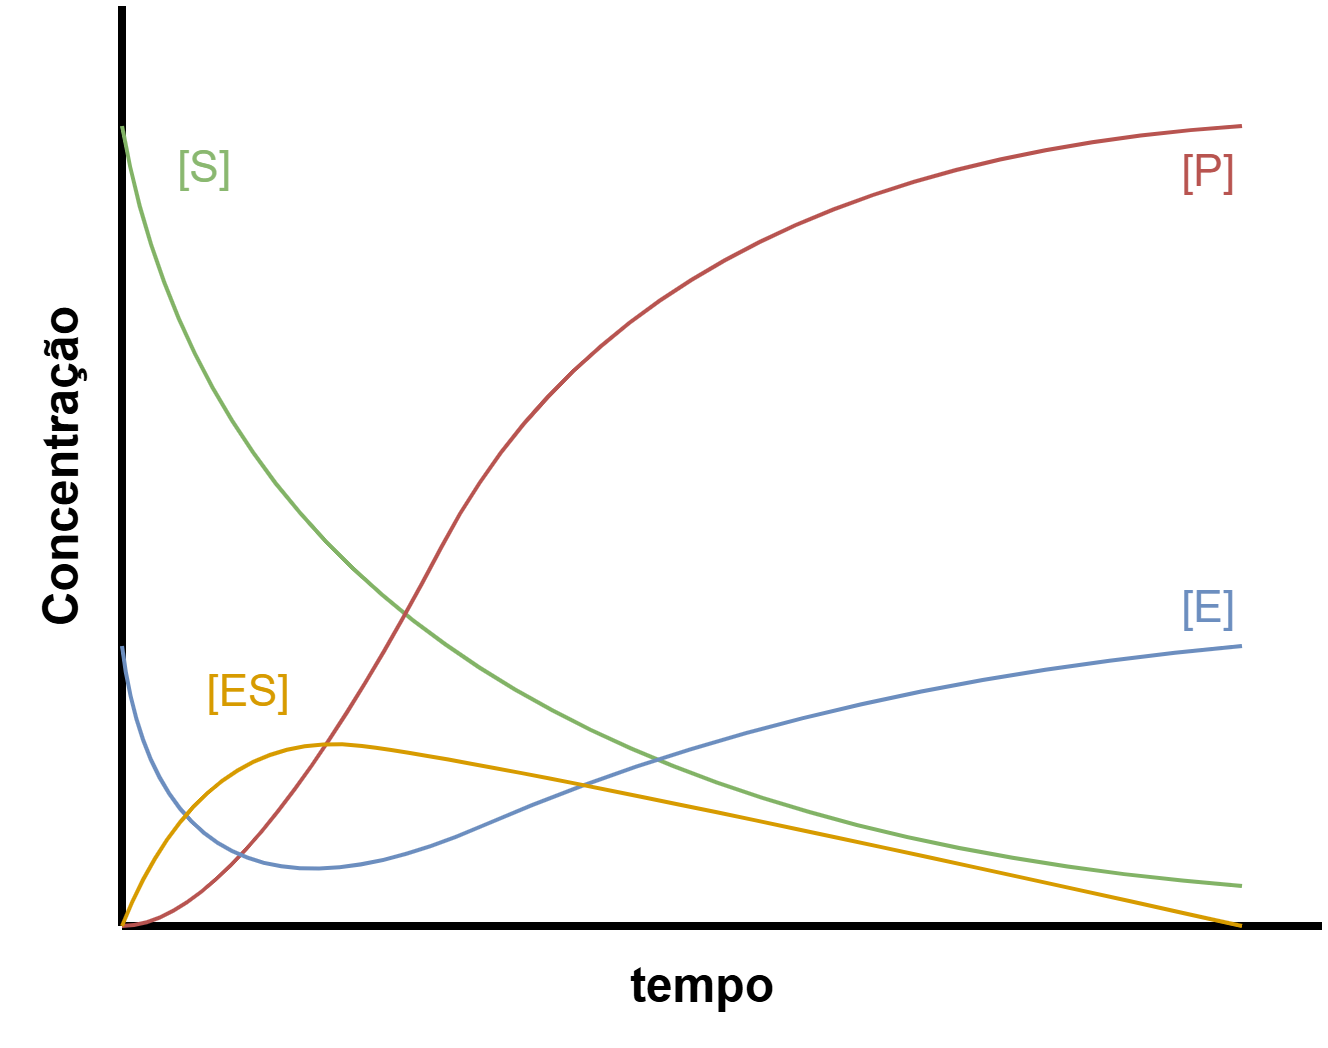
\includegraphics[width=0.6\textwidth]{img/conc_time.png}
    \caption{\small Tendências típicas das concentrações de enzima, substrato, complexo e produto ao longo do tempo em uma reação enzimática de Michaelis-Menten. Fonte: Adaptado de Wikipedia \cite{file_michaelis_menten_sp_e_es}.}
    \label{fig:concentracoes_michaelis_menten}
\end{figure}

Experimentalmente, é comum tentar determinar os parâmetros cinéticos de uma enzima, como $V_{max}$ e $K_m$, por meio da chamada \textit{Curva de Michaelis-Menten}, que é um gráfico da taxa da reação (ou taxa de formação de produto) contra a concentração de substrato, ou pelo chamado método de \textit{Lineweaver-Burk}, que lineariza a correlação entre as mesmas duas variáveis. As Figuras \ref{fig:MM_plot} e \ref{fig:lineweaver_burk} mostram, respectivamente, a curva de Michaelis-Menten e o gráfico de Lineweaver-Burk típicos.

\begin{figure}[H]
    \centering
    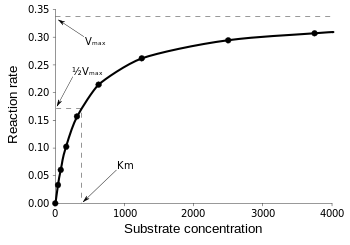
\includegraphics[width=0.6\textwidth]{img/Vmax_Km.png}
    \caption{\small Curva de Michaelis-Menten típica, utilizada para determinar as constantes $K_M$ e $V_{max}$. Fonte: \citetitle{libretexts_michaelis_menten}.}
    \label{fig:MM_plot}
\end{figure}

\begin{figure}[H]
    \centering
    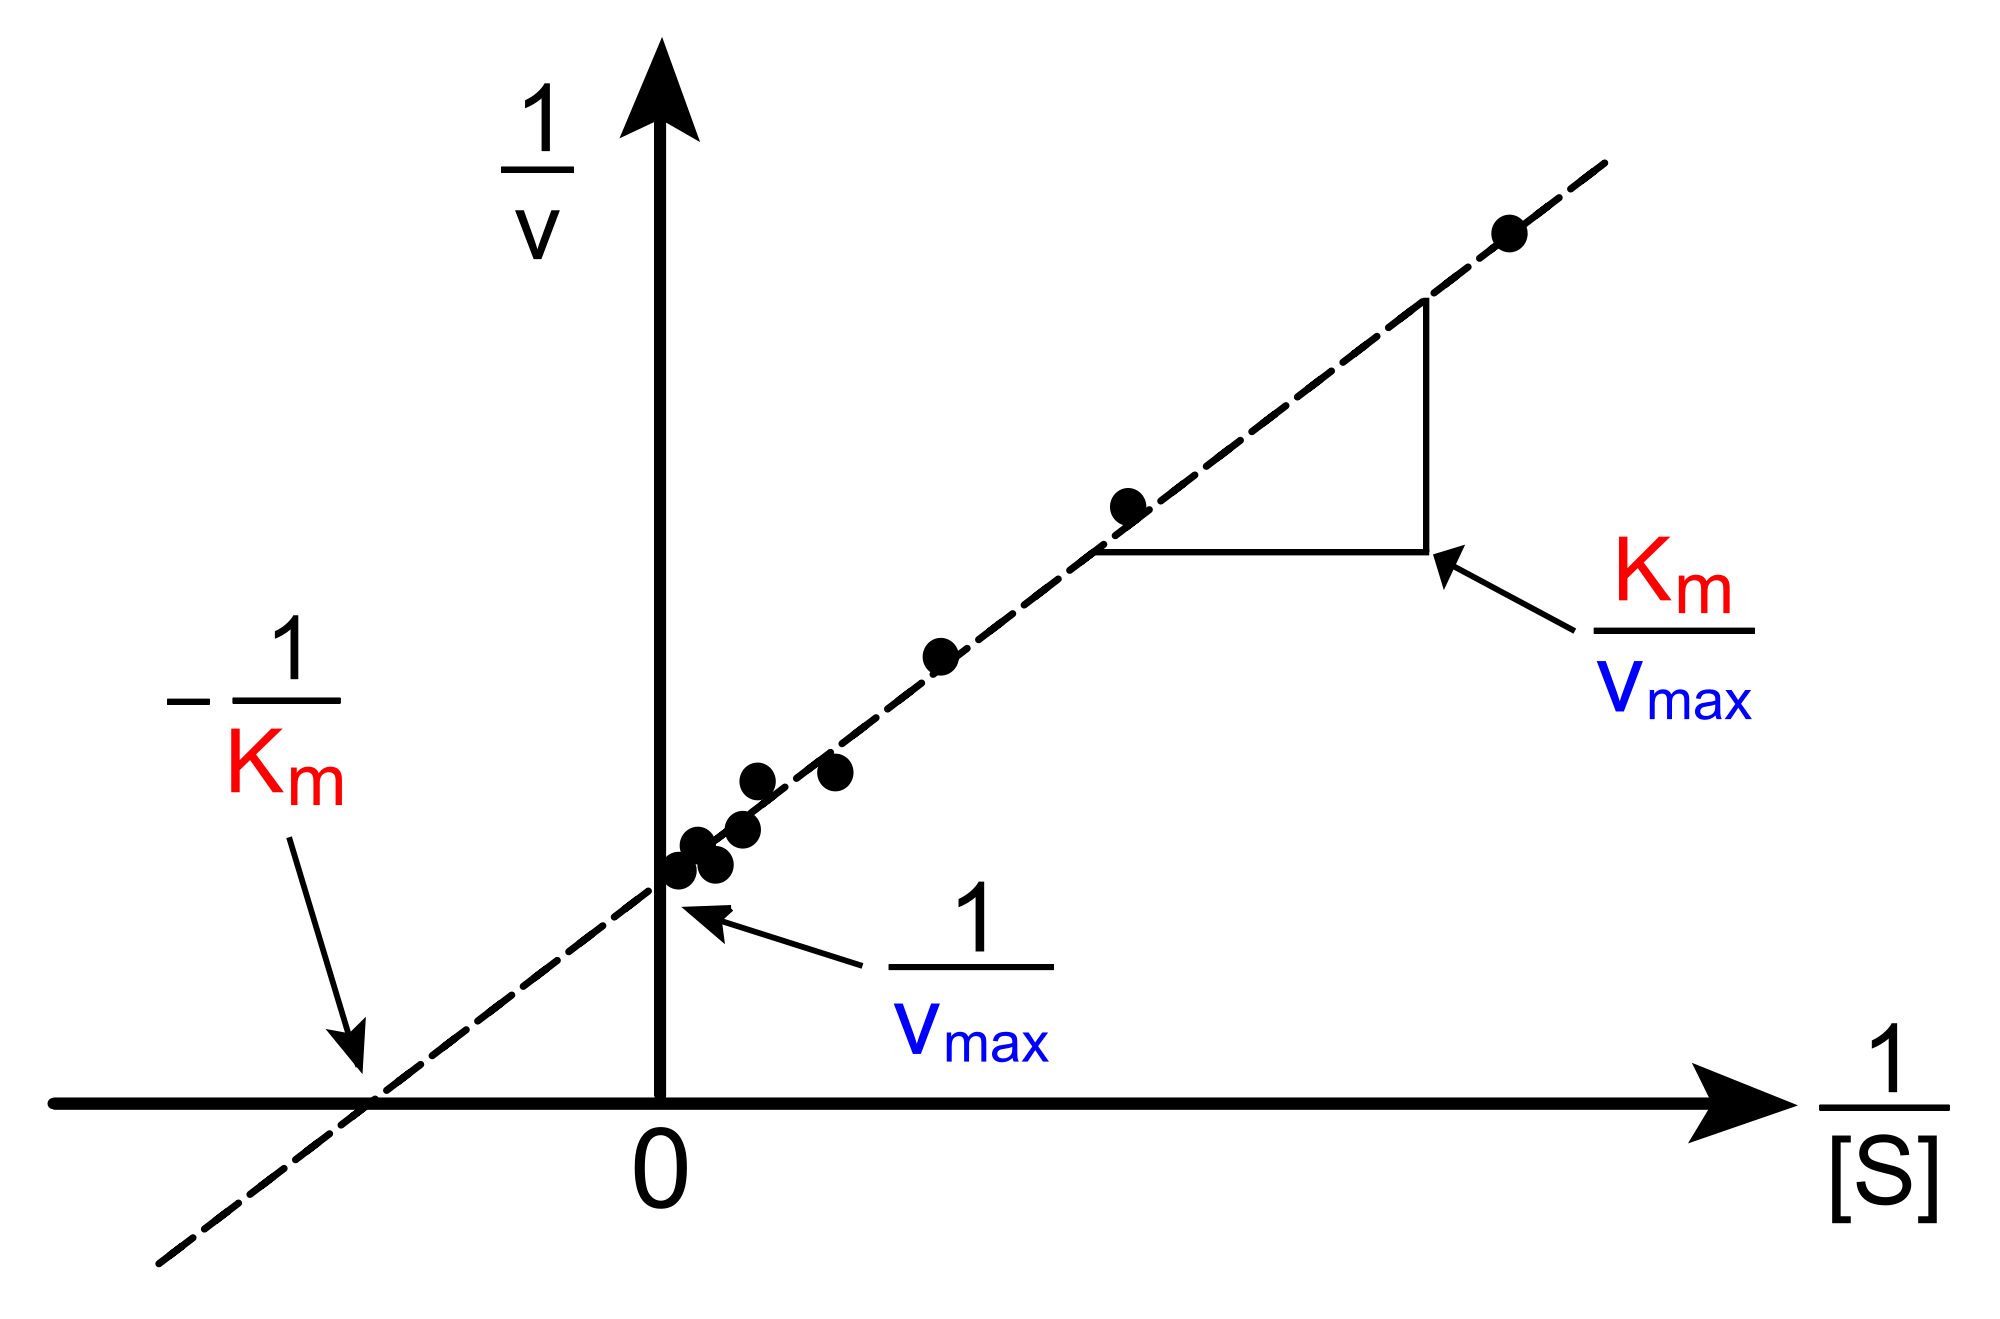
\includegraphics[width=0.6\textwidth]{img/LB.png}
    \caption{\small Gráfico típico Lineweaver-Burk, utilizado para determinar as constantes $K_M$ e $V_{max}$. Fonte: \citetitle{libretexts_michaelis_menten}.}
    \label{fig:lineweaver_burk}
\end{figure}

Além do modelo básico de Michaelis-Menten, é fundamental considerar os efeitos de inibidores, que podem estar presentes no meio reacional, seja como contaminantes, subprodutos ou aditivos intencionais. Os principais tipos de inibição são: competitiva, não competitiva e acompetitiva. Na inibição competitiva, o inibidor compete com o substrato pelo sítio ativo da enzima, elevando o valor aparente de
$K_m$ sem alterar $V_{max}$ \cite{FOGLER_2016}.

Já na inibição não competitiva, o inibidor se liga a um sítio diferente do sítio ativo, reduzindo $V_{max}$ sem afetar $K_m$. Na inibição acompetitiva, o inibidor se liga apenas ao complexo $ES$, reduzindo tanto $V_{max}$ quanto $K_m$ \cite{FOGLER_2016}.

A Figura \ref{fig:inibicao} ilustra os efeitos da inibição competitiva e não competitiva na curva de Michaelis-Menten. A presença de inibidores altera a dinâmica da reação, impactando diretamente a eficiência do processo enzimático.

\begin{figure}[H]
    \centering
    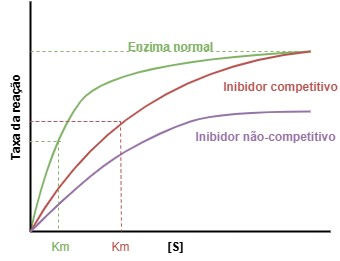
\includegraphics[width=0.5\textwidth]{img/inibicao.png}
    \caption{\small Efeitos da inibição competitiva e não competitiva na curva de Michaelis-Menten. Fonte: Autoria própria.}
    \label{fig:inibicao}
\end{figure}

Outro mecanismo relevante, especialmente em reações envolvendo múltiplos substratos e produtos, é o mecanismo ping-pong-bi-bi. Nesse mecanismo, a enzima alterna entre diferentes estados intermediários, transferindo grupos funcionais de um substrato para outro em etapas sequenciais. O esquema geral pode ser representado como:

\begin{equation}
    \begin{aligned}
        E + A \rightarrow EA \rightarrow E' + P \\
        E' + B \rightarrow E'B \rightarrow E + Q
    \end{aligned}
\end{equation}
onde $A$ e $B$ são substratos, $P$ e $Q$ são produtos, $E$ é a enzima em seu estado original e $E'$ é a enzima modificada após a reação com o primeiro substrato. Esse mecanismo é típico de enzimas transferases e algumas oxidoredutases, sendo importante em processos industriais que envolvem reações de transferência de grupos funcionais \cite{FOGLER_2016}.

O conhecimento detalhado desses mecanismos permite a modelagem matemática precisa dos processos enzimáticos, possibilitando a simulação, o controle e a otimização de reatores industriais. Além disso, a compreensão dos fatores que afetam a atividade enzimática, como concentração de substrato, presença de inibidores e condições físico-químicas do meio, é fundamental para o desenvolvimento de processos robustos e eficientes.

\subsection{Reações Enzimáticas em Meios Multifásicos}

As reações enzimáticas em sistemas multifásicos, especialmente em meios aquoso-orgânicos, representam uma abordagem consolidada para ampliar o alcance de substratos processáveis, particularmente aqueles de natureza hidrofóbica ou com baixa solubilidade em água. Nesses sistemas, a enzima permanece majoritariamente na fase aquosa, enquanto o substrato e/ou produto se concentram preferencialmente na fase orgânica, facilitando tanto o uso de compostos insolúveis quanto a separação in situ dos produtos. Entretanto, a eficiência global da transformação depende não apenas da transferência de massa entre as fases, mas também da manutenção da estrutura conformacional da enzima, a qual é fortemente influenciada pela quantidade e pela atividade termodinâmica de água no meio \cite{verger_action_1973} \cite{reis_lipases_2009}.

O modelo de Michaelis-Menten, embora amplamente utilizado, apresenta limitações quando aplicado a sistemas multifásicos. Ao deduzir as expressões de taxa de reação para esse modelo, implicitamente assume-se que a enzima e o substrato estão na mesma fase, em meio homogêneo. No entanto, em sistemas bifásicos, essa suposição não se sustenta, uma vez que a enzima está predominantemente na fase aquosa, enquanto o substrato pode estar na fase orgânica \cite{andersen_michaelis_2018}.

Estudos pioneiros de Klibanov \cite{klibanov} e colaboradores demonstraram que enzimas mantêm atividade catalítica significativa mesmo em solventes praticamente anidros, desde que se preserve uma monocamada de água firmemente adsorvida à superfície proteica – fenômeno conhecido como “pH-memory” – e se controlem parâmetros como a atividade de água (a\textsubscript{w}) e o log P do solvente, que afetam diretamente a flexibilidade intrínseca do biocatalisador e, consequentemente, sua atividade catalítica \cite{klibanov}.

Adicionalmente, a escolha do solvente orgânico exerce papel decisivo: solventes com log P elevado (\textgreater 4) tendem a ser menos desnaturantes, enquanto solventes de polaridade intermediária ($0 < log P < 2$) podem provocar rápida inativação enzimática. A engenharia de solventes, portanto, possibilita modular não só a estabilidade térmica, mas também a especificidade estereo-, regio- e quimiosseletiva da enzima, tornando viável a obtenção de rendimentos e produtividades competitivos em escala industrial. Assim, a adoção de sistemas bifásicos ou mesmo de meios predominantemente orgânicos – quando devidamente ajustados quanto à a\textsubscript{w}, à força iônica residual e à presença de eventuais co-solventes ou aditivos protetores – oferece uma plataforma robusta para a síntese de intermediários finos, fragrâncias, fármacos e polímeros, expandindo consideravelmente o campo de aplicação da catálise enzimática além do escopo tradicionalmente aquoso \cite{klibanov}.

A interface entre as fases assume papel central nesses sistemas, pois é nela que ocorre a transferência de substrato da fase orgânica para a fase aquosa, onde a enzima está ativa. A área interfacial disponível, a natureza química das fases e a presença de agentes interfaciais influenciam diretamente a taxa de reação. Em muitos casos, a transferência de massa pode se tornar o fator limitante do processo, especialmente quando a solubilidade do substrato na fase aquosa é muito baixa. Para contornar esse desafio, técnicas como agitação vigorosa, uso de reatores especiais (como reatores de leito fluidizado) e, principalmente, a adição de surfactantes são empregadas para aumentar a área interfacial e promover emulsificação \cite{schmid2002enzyme}.

Surfactantes são moléculas anfifílicas que, ao serem adicionadas a sistemas multifásicos, reduzem a tensão interfacial entre as fases e promovem a formação de micelas, emulsões ou microemulsões. Essas estruturas aumentam significativamente a área de contato entre as fases, facilitando a difusão do substrato até a enzima e, consequentemente, aumentando a taxa de reação. Além disso, surfactantes podem atuar como agentes estabilizantes para as enzimas, protegendo-as contra desnaturação causada pelo contato direto com solventes orgânicos ou pela adsorção na interface. Em sistemas de microemulsão, por exemplo, as enzimas podem ser encapsuladas em gotículas aquosas dispersas em uma fase contínua orgânica, o que proporciona um ambiente aquoso favorável à sua atividade, mesmo em presença de solventes potencialmente desnaturantes \cite{lau2010surfactants}.

O efeito dos surfactantes sobre a atividade enzimática, entretanto, é altamente dependente de sua natureza química, concentração e do tipo de enzima utilizada. Surfactantes aniônicos, catiônicos, não iônicos e zwitteriônicos podem interagir de maneiras distintas com a superfície da enzima, podendo tanto estabilizá-la quanto inibi-la. Em concentrações adequadas, surfactantes não iônicos, como o Triton X-100 ou o Tween 80, são frequentemente utilizados para aumentar a solubilidade de substratos hidrofóbicos e proteger a estrutura enzimática. Por outro lado, concentrações excessivas ou o uso de surfactantes com alta afinidade pela superfície proteica podem levar à desnaturação, agregação ou inativação da enzima, prejudicando o desempenho do processo \cite{lau2010surfactants}.

Além do papel na transferência de massa e estabilização, surfactantes podem modular a seletividade da reação enzimática, influenciando a orientação do substrato na interface e, consequentemente, o perfil de produtos obtidos. Isso é particularmente relevante em reações de síntese orgânica fina, como a produção de ésteres, onde a seletividade enzimática pode ser ajustada por meio da escolha do tipo e da concentração de surfactante. Em alguns casos, a presença de surfactantes permite a realização de reações reversas, como a síntese de ligações peptídicas ou ésteres em meio orgânico, ampliando ainda mais as possibilidades de aplicação industrial das enzimas \cite{lau2010surfactants}.

A concentração micelar crítica (CMC) representa um ponto-chave em sistemas enzimáticos que envolvem interfaces, como micelas e membranas. Ao se atingir a CMC, moléculas anfifílicas, como surfactantes ou certos substratos, passam a formar micelas de maneira espontânea. Essas estruturas micelares criam ambientes diferenciados onde as reações enzimáticas podem ocorrer. Nesse cenário, a cinética das enzimas é impactada, pois a quantidade de substrato disponível para a catálise depende do equilíbrio entre a fase aquosa e a interface micelar. Acima da CMC, a fração de substrato acessível à enzima se estabiliza, permitindo que a equação de Michaelis--Menten seja adaptada para descrever a saturação da interface \cite{bisswanger2017}.

Em sistemas interfaciais, a CMC marca a transição em que o aumento da concentração total de substrato não resulta mais em maior disponibilidade para a enzima, já que o excesso de substrato é incorporado às micelas. Isso influencia diretamente a determinação dos parâmetros cinéticos, como Km e Vmax, que precisam ser analisados considerando a distribuição do substrato entre as diferentes fases do sistema. Assim, compreender o conceito de CMC é fundamental para projetar e interpretar experimentos com enzimas em meios micelares ou membranosos, sendo um aspecto central para a modelagem e otimização de processos enzimáticos em ambientes heterogêneos \cite{bisswanger2017}.

Portanto, o desenvolvimento de processos enzimáticos eficientes em meios multifásicos requer uma compreensão aprofundada dos fenômenos interfaciais, da dinâmica de transferência de massa e das interações entre enzimas, surfactantes e solventes. A escolha criteriosa dos componentes do sistema, aliada ao controle das condições operacionais, é fundamental para garantir alta atividade, estabilidade e seletividade enzimática, viabilizando aplicações industriais inovadoras e sustentáveis.

\section{SIMULAÇÃO COM AUTÔMATOS CELULARES}

\subsection{Breve Histórico e Aplicações}

A concepção dos autômatos celulares remonta aos anos 1940, com os trabalhos pioneiros de John von Neumann e Stanisław Ulam, que buscavam modelos para sistemas autorreprodutores e o crescimento de cristais, respectivamente. No entanto, foi com o matemático John Conway, na década de 1970, que os autômatos celulares ganharam notoriedade com a criação do ``Jogo da Vida'' (Conway's Game of Life) \cite{Gardner1970}. O ``Jogo da Vida'' é um autômato celular bidimensional com regras extremamente simples: uma célula viva com menos de dois vizinhos vivos morre por subpopulação; uma célula viva com dois ou três vizinhos vivos sobrevive para a próxima geração; uma célula viva com mais de três vizinhos vivos morre por superpopulação; e uma célula morta com exatamente três vizinhos vivos se torna uma célula viva por reprodução. Apesar da simplicidade das regras, o ``Jogo da Vida'' é capaz de gerar padrões complexos e dinâmicos, incluindo estruturas que se movem, se replicam e interagem, demonstrando o poder dos ACs para simular fenômenos emergentes \cite{Gardner1970}.

Além do ``Jogo da Vida'', os autômatos celulares encontraram aplicações em uma vasta gama de áreas. Na física, são utilizados para modelar fenômenos como a formação de padrões em fluidos e a propagação de incêndios florestais. Na biologia, são empregados para simular o crescimento de populações, a propagação de doenças e o desenvolvimento embrionário. A versatilidade dos autômatos celulares reside na sua capacidade de capturar a essência da interação local e sua emergência em comportamentos globais, tornando-os uma ferramenta valiosa para a compreensão e simulação de sistemas complexos em diversas disciplinas \cite{kier2005}.

\subsection{Definição}

Autômatos Celulares (AC) representam um paradigma computacional discreto que modela sistemas complexos através da interação local de componentes simples. Essencialmente, um autômato celular consiste em uma grade regular de células, onde cada célula possui um estado finito e discreto. A evolução do sistema ocorre em passos de tempo discretos, e o estado de cada célula no próximo passo de tempo é determinado por uma regra de transição que leva em consideração o seu próprio estado atual e os estados de suas células vizinhas. Essa regra é aplicada de forma síncrona e uniforme a todas as células da grade. A simplicidade das regras locais, quando aplicadas em larga escala, pode gerar comportamentos globais extremamente complexos e emergentes, tornando os ACs ferramentas poderosas para a simulação de fenômenos diversos \cite{kier2005}.

Os autômatos celulares são frequentemente representados por uma grade multidimensional, onde cada célula pode assumir um de vários estados possíveis. A configuração mais comum é a grade bidimensional, mas também podem ser utilizados grades unidimensionais ou tridimensionais. Para este trabalho, são utilizadas grades bidimensionais e os estados possíveis de uma célula são representados por \textbf{componentes}, que possuem significado físico, ou por \textbf{vazios}. A Figura \ref{fig:grade_2d} ilustra uma grade 2D (bidimensional) 5 x 5, isto é, de 5 linhas e 5 colunas.

\begin{figure}[H]
    \centering
    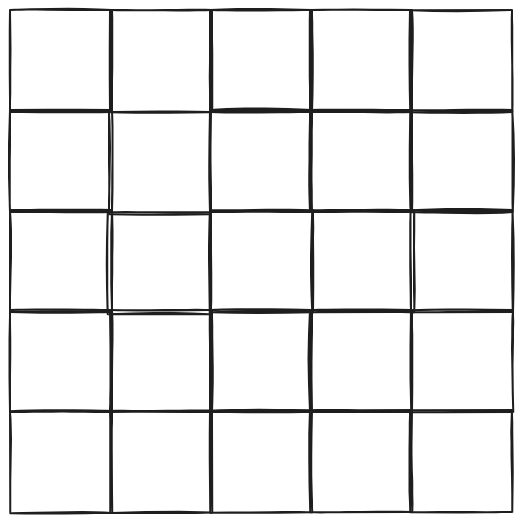
\includegraphics[width=0.5\textwidth]{img/grade_2d.png}
    \caption{\small Exemplo de autômato celular 2D (5 x 5) com células representando vazios.}
    \label{fig:grade_2d}
\end{figure}

Os componentes são entidades que efetivamente ocupam células da grade e podem representar diferentes espécies químicas, como enzimas, substratos ou produtos. Cada componente pode ter propriedades específicas, como taxa de reação, probabilidade de movimentação e afinidade por outros componentes. Os vazios representam células desocupadas na grade, onde componentes podem se mover ou interagir. A dinâmica do autômato celular é governada por regras de transição que determinam como os estados das células evoluem ao longo do tempo, com base nas interações entre componentes e vazios. Essas regras podem ser definidas de maneira a simular processos químicos, biológicos ou físicos, permitindo a modelagem de sistemas complexos de forma eficiente e intuitiva \cite{kier2005}.

Células de componentes podem interagir com suas vizinhas por meio de regras válidas igualitariamente independente de uma orientação no espaço, mas também podem ser definidas regras que dependem da orientação. Quando se deseja definir diferentes regras de interação dependendo de uma orientação, é interessante utilizar um estado rotacionável, que pode assumir diferentes orientações. Dessa forma, pelo menos um lado de uma mesma célula pode interagir de forma distinta em comparação aos outros lados. A Figura \ref{fig:celula_rotacionavel} ilustra uma célula rotacionável com quatro orientações possíveis. O lado A1 pode interagir com regras e valores distintos dos outros três lados, identificados em conjunto com o rótulo A2.

\begin{figure}[H]
    \centering
    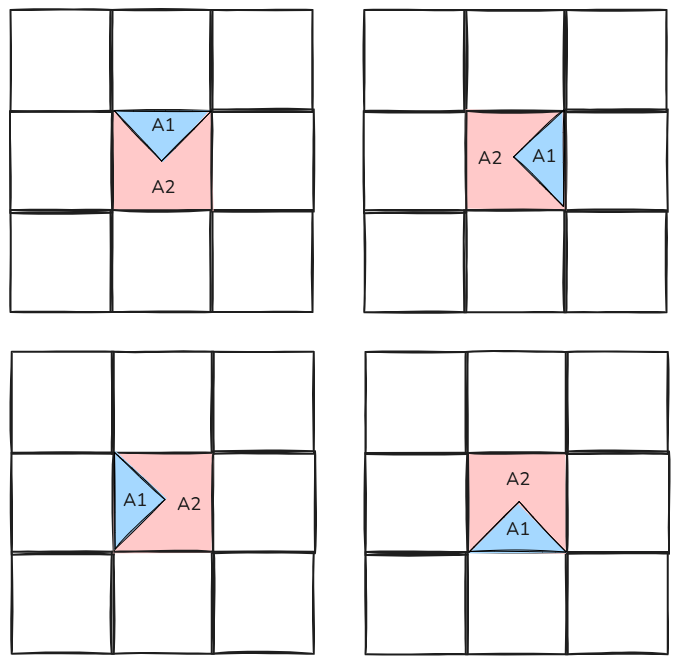
\includegraphics[width=0.5\textwidth]{img/componente_rotaciona.png}
    \caption{\small Exemplo de célula rotacionável com quatro orientações possíveis.}
    \label{fig:celula_rotacionavel}
\end{figure}

As células interagem com suas vizinhas imediatas, que podem ser definidas de diferentes maneiras. A vizinhança mais comum é a \textit{vizinhança de von Neumann}, que inclui as quatro células adjacentes (cima, baixo, esquerda e direita) pintadas de azul na Figura \ref{fig:vizinhanca_von_neumann}. A \textit{vizinhança de von Neumann estendida}, por sua vez, inclui também as células pintadas de verde na Figura \ref{fig:vizinhanca_von_neumann_estendida}, totalizando oito células vizinhas. Também é possível definir outras vizinhanças, como a \textit{vizinhança de Moore}, que inclui todas as oito células adjacentes (cima, baixo, esquerda, direita e as quatro diagonais), como na Figura \ref{fig:vizinhanca_moore}. A escolha da vizinhança influencia diretamente a dinâmica do autômato celular e, consequentemente, o comportamento emergente do sistema simulado. Neste trabalho são utilizadas as vizinhanças de von Neumann e von Neumann estendida.

\begin{figure}[H]
    \centering
    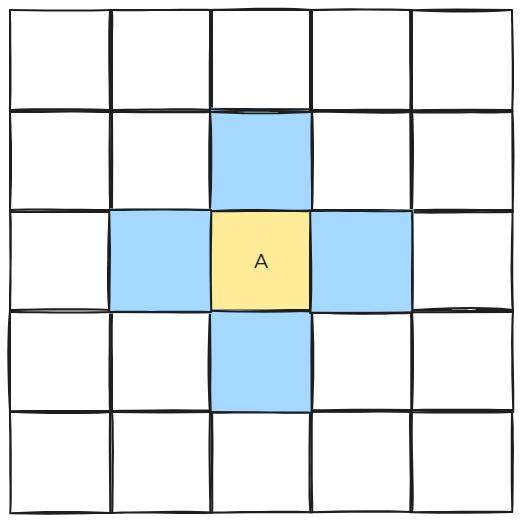
\includegraphics[width=0.5\textwidth]{img/vizinhanca_von_neumann.png}
    \caption{\small Vizinhança de von Neumann de um componente A, definida pelas 4 células azuis.}
    \label{fig:vizinhanca_von_neumann}
\end{figure}

\begin{figure}[H]
    \centering
    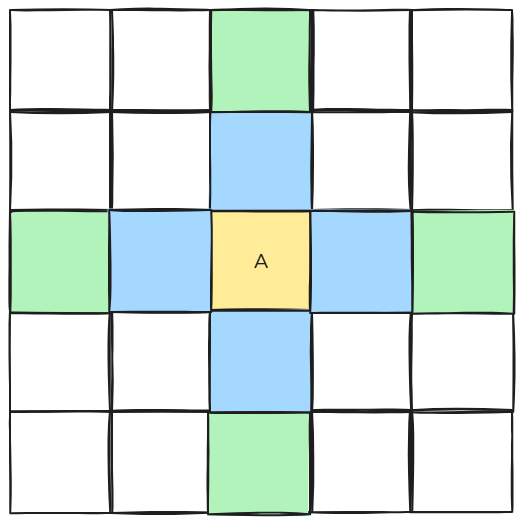
\includegraphics[width=0.5\textwidth]{img/vizinhanca_von_neumann_estendida.png}
    \caption{\small Vizinhança de von Neumann estendida de um componente A, definida pelas células azuis e verdes.}
    \label{fig:vizinhanca_von_neumann_estendida}
\end{figure}

\begin{figure}[H]
    \centering
    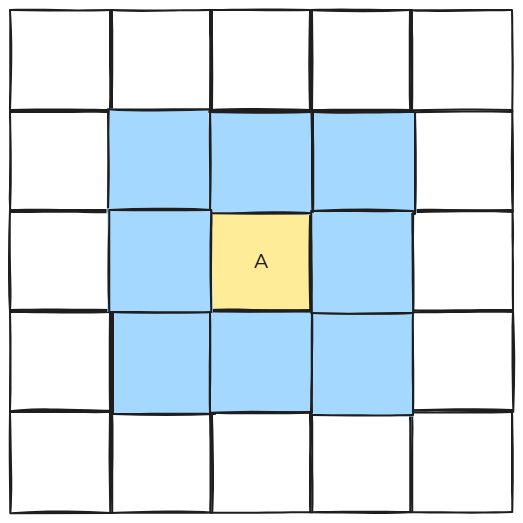
\includegraphics[width=0.5\textwidth]{img/vizinhanca_moore.png}
    \caption{\small Vizinhança de Moore de um componente A, definida pelas 8 células azuis.}
    \label{fig:vizinhanca_moore}
\end{figure}

Os modelos de autômato celular (AC) empregados neste trabalho seguem predominantemente o formalismo probabilístico descrito por Kier \cite{kier2005}. Cada componente ou vazio ocupa uma célula de uma malha quadrada e interage apenas com as células de sua \textit{vizinhança de von Neumann estendida}. A dinâmica emerge da aplicação sincrônica, a cada iteração, (i) das \textbf{regras de movimentação} e (ii) das \textbf{regras de transição}. A seguir são definidos os cinco parâmetros fundamentais desses conjuntos de regras: $P_M$, $P_B$, $J$, $P_R$ e $P_{rot}$.

\subsubsection{Probabilidade de Movimentação Livre – \texorpdfstring{$P_M$}{Pm}}
\label{subsubsec:Pm}

\begin{itemize}
    \item \textbf{Definição:} $P_M$ representa a chance de um componente isolado se mover para uma célula desocupada de sua vizinhança de von Neumann (Figura \ref{fig:movimentacao_livre}). Essa probabilidade é influenciada por fatores como a densidade de componentes nas células vizinhas e a natureza do próprio componente.
    \item \textbf{Intervalo:} $0 \le P_M \le 1$.
    \item \textbf{Interpretação física:} controla a \textit{mobilidade inerente}.
          Valores próximos de 1 reproduzem um passeio aleatório praticamente livre; valores
          menores simulam espécies mais lentas.
\end{itemize}

\begin{figure}[H]
    \centering
    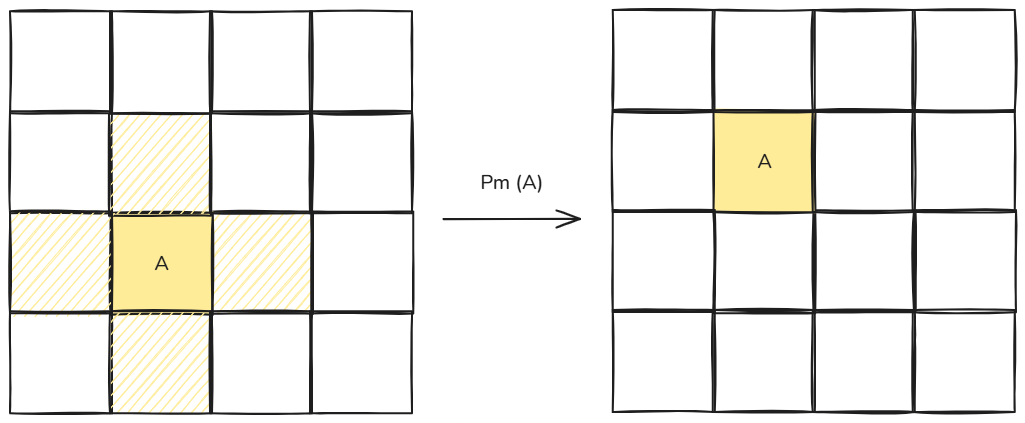
\includegraphics[width=0.8\textwidth]{img/Pm.png}
    \caption{\small Exemplo de movimentação livre de um componente A para uma célula vazia da sua vizinhança de von Neumann.}
    \label{fig:movimentacao_livre}
\end{figure}

\subsubsection{Parâmetro de Junção – \texorpdfstring{$J$}{J}}
\label{subsubsec:J}

\begin{itemize}
    \item \textbf{Definição:} $J(AB)$ modula a
          \emph{propensão de movimento de $A$ na direção de $B$}
          quando ambos estão separados por exatamente uma célula vazia. A Figura \ref{fig:movimentacao_juncao} ilustra essa situação, onde $A$ possui um vazio em sua vizinhança de von Neumann e este vazio separa $A$ de $B$ que, por sua vez, está na vizinhança de von Neumann estendida de $A$.
    \item \textbf{Valores típicos:}
          \[
              J(AB)=
              \begin{cases}
                  >1    & \text{atração curta distância}  \\[2pt]
                  =1    & \text{deslocamento indiferente} \\[2pt]
                  0<J<1 & \text{repulsão}                 \\[2pt]
                  =0    & \text{movimento proibido}
              \end{cases}
          \]
    \item \textbf{Significado químico:} descreve interações
          hidrofóbicas/hidrofílicas, cargas opostas, etc.
          Por exemplo, \citeauthor{kier2005} ajustam
          $J(\mathrm{WW})>1$ para reproduzir a coesão da água líquida.
\end{itemize}

\begin{figure}[H]
    \centering
    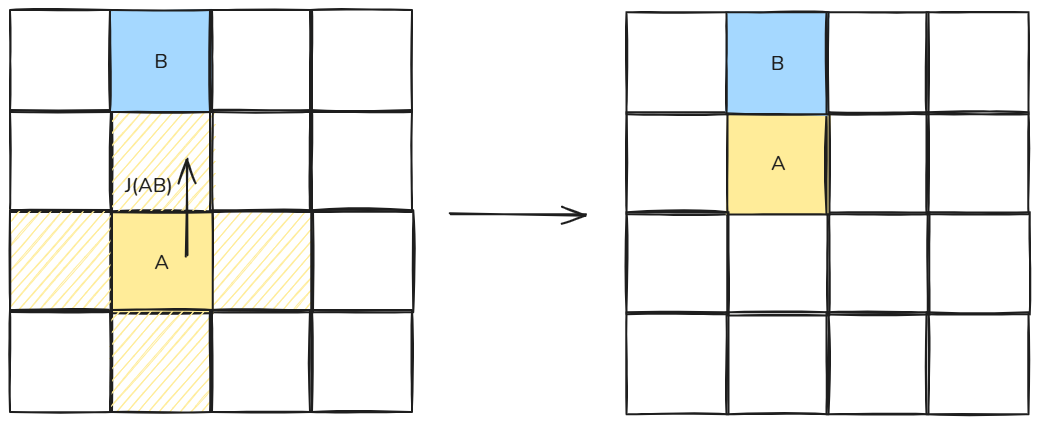
\includegraphics[width=0.8\textwidth]{img/Jab.png}
    \caption{\small Exemplo de movimentação de um componente A na direção de um componente B, separados por uma célula vazia, com propensão de movimento $J(AB)$.}
    \label{fig:movimentacao_juncao}
\end{figure}

\subsubsection{Probabilidade de Quebra – \texorpdfstring{$P_B$}{Pb}}
\label{subsubsec:Pb}

\begin{itemize}
    \item \textbf{Definição:} $P_B(AB)$ é a probabilidade de
          \emph{separação} de dois componentes adjacentes $A$ e $B$
          (``quebra de ligação'') em uma iteração. A Figura \ref{fig:quebra_ligacao} ilustra essa situação, onde $B$ está em uma célula adjacente a $A$.
    \item \textbf{Intervalo:} $0 \le P_B \le 1$.
    \item \textbf{Coesão:} $P_B=0$ \,($A$ e $B$ nunca se separam)
          $\rightarrow$ forte coesão;
          $P_B=1$ \,($A$ e $B$ sempre se separam) $\rightarrow$ ligação fraca.
    \item \textbf{Dependência de coordenação:} se $A$ está ligado a
          $n$ vizinhos do tipo $B$, a probabilidade conjunta de separação é
          $P_B^{\,n}$; logo, múltiplos contatos estabilizam o agregado.
    \item \textbf{Correspondência físico-química:}
          em água, $P_B(\mathrm{WW})$ pode ser correlacionado com a temperatura:
          valores maiores a temperaturas elevadas representam a maior
          desordem da rede de ligações de hidrogênio \cite{kier2005}.
\end{itemize}

\begin{figure}[H]
    \centering
    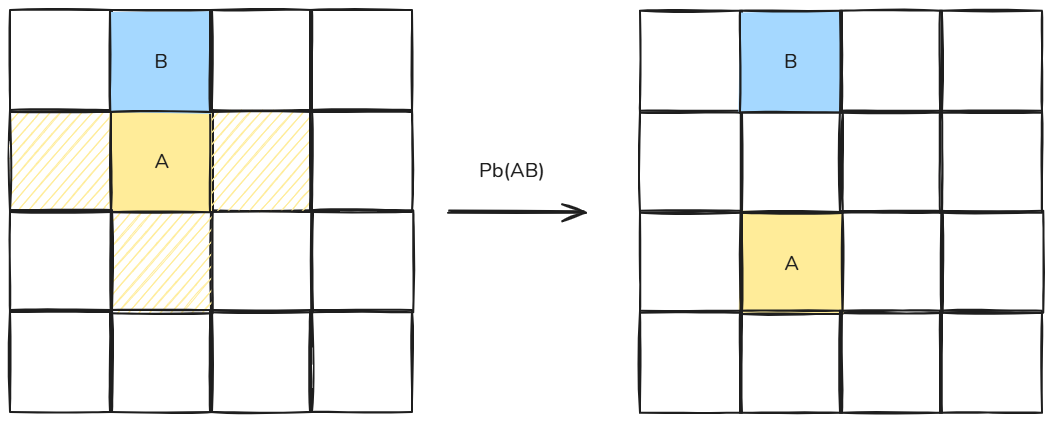
\includegraphics[width=0.8\textwidth]{img/PbAB.png}
    \caption{\small Exemplo de quebra de ligação entre dois componentes A e B adjacentes, com probabilidade de quebra $P_B(AB)$.}
    \label{fig:quebra_ligacao}
\end{figure}

\subsubsection{Probabilidade de Reação – \texorpdfstring{$P_R$}{Pr}}
\label{subsubsec:Pr}

\begin{itemize}
    \item \textbf{Definição:} $P_R$ (substitui o símbolo $P_t$ de
          \citeauthor{kier2005}) é a probabilidade de conversão química
          durante uma iteração. A Figura \ref{fig:reacao} ilustra essa situação, onde $A$ e $B$ estão em células adjacentes e podem reagir para formar $C$ e $D$.
    \item \textbf{Intervalo:} $0 \le P_R \le 1$.
    \item \textbf{Reações elementares:} $P_R$ é aplicado a
          \emph{reações elementares} que ocorrem quando
          dois componentes estão em células adjacentes.
          Por exemplo, $A+B \xrightarrow{P_R(AB)} C+D$
          representa a reação entre $A$ e $B$ para formar $C$ e $D$ com probabilidade $P_R(AB)$.
    \item \textbf{Casos de uso:}
          \begin{enumerate}
              \item \emph{Transição de primeira ordem:}
                    $A \xrightarrow{P_R(A\rightarrow B)} B$.\\
                    Se $P_R=1$ a transição é determinística;
                    $0<P_R<1$ torna-a estocástica.
              \item \emph{Reação de encontro (segunda ordem):}\\
                    quando $A$ e $B$ tornam-se vizinhos,
                    ocorre $A+B \xrightarrow{P_R(AB)} C+D$
                    com probabilidade $P_R(AB)$.
          \end{enumerate}
    \item \textbf{Significado cinético:} $P_R$ pode ser relacionado a
          uma constante de velocidade efetiva $k$
          (\textit{via} calibração: $k = P_R/\Delta t$,
          onde $\Delta t$ é a duração de uma iteração).
    \item \textbf{Importância prática:}
          em modelos enzimáticos, por exemplo, $P_R(\mathrm{AB})$
          controla a etapa catalítica $\mathrm{ES}\rightarrow\mathrm{EP}$
          e permite reproduzir curvas de Michaelis–Menten
          \cite[cap.~9]{kier2005}.
\end{itemize}

\begin{figure}[H]
    \centering
    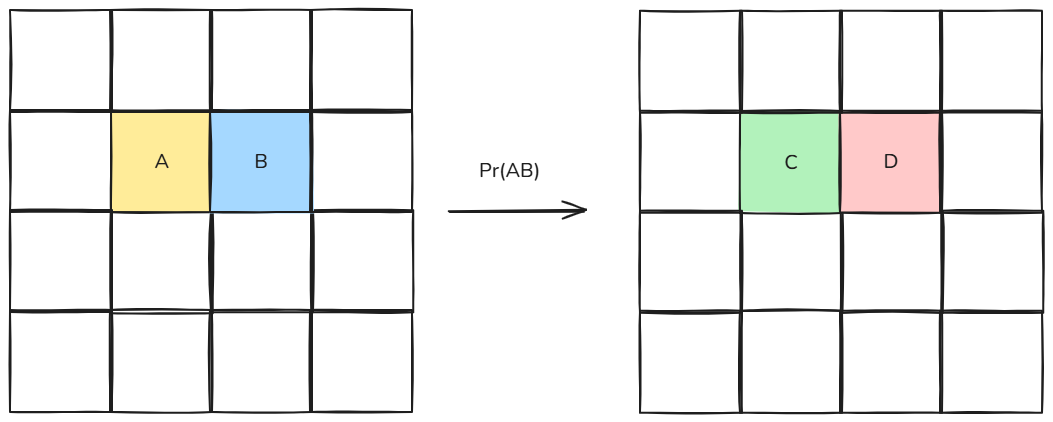
\includegraphics[width=0.8\textwidth]{img/reacao.png}
    \caption{\small Exemplo de reação entre dois componentes A e B adjacentes, formando C e D com probabilidade de reação $P_R(AB)$.}
    \label{fig:reacao}
\end{figure}

\subsubsection{Probabilidade de Rotação – \texorpdfstring{$P_{rot}$}{Prot}}
\label{subsubsec:Prot}

\begin{itemize}
    \item \textbf{Definição:} $P_{rot}$ é a probabilidade de um componente rotacionar sua orientação em uma iteração (Figura \ref{fig:rotacao}). Essa rotação pode ser necessária para alinhar o componente com outros vizinhos ou para otimizar a interação com o meio.
    \item \textbf{Intervalo:} $0 \le P_{rot} \le 1$.
    \item \textbf{Significado físico:} controla a flexibilidade do componente, permitindo que ele se adapte à configuração espacial dos vizinhos.
    \item \textbf{Aplicações:} útil em simulações onde a orientação espacial dos componentes influencia suas interações, como sistemas biológicos complexos.
\end{itemize}

\begin{figure}[H]
    \centering
    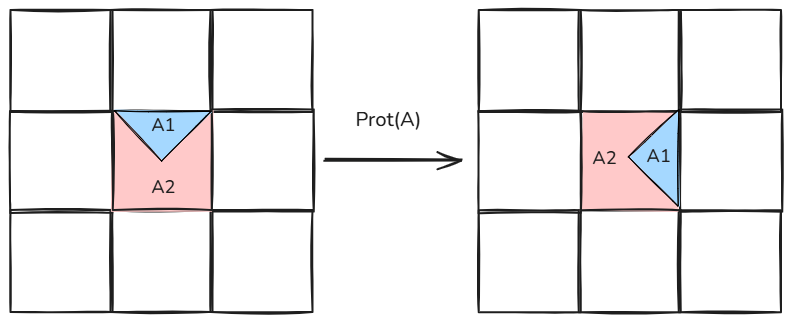
\includegraphics[width=0.8\textwidth]{img/rotacao.png}
    \caption{\small Exemplo de rotação de um componente A com probabilidade de rotação $P_{rot}$.}
    \label{fig:rotacao}
\end{figure}

\begin{table}[H]
    \centering
    \caption{Parâmetros Fundamentais do Modelo de Autômato Celular}
    \vspace{0.2cm}
    \begin{tabularx}{\textwidth}{X m{3cm} m{3cm}}
        \hline
        \textbf{Parâmetro}                  & \textbf{Símbolo} & \textbf{Intervalo}      \\
        \hline
        Probabilidade de movimentação livre & $P_M$            & $0 \leq P_M \leq 1$     \\
        Probabilidade de quebra             & $P_B$            & $0 \leq P_B \leq 1$     \\
        Parâmetro de junção                 & $J$              & $0 \leq J < \infty$     \\
        Probabilidade de reação             & $P_R$            & $0 \leq P_R \leq 1$     \\
        Probabilidade de rotação            & $P_{rot}$        & $0 \leq P_{rot} \leq 1$ \\
        \hline
    \end{tabularx}

    \vspace{0.2cm}
    \makebox[\linewidth][l]{\small Fonte: Autoria própria}
\end{table}

\subsubsection{Fração de Células Vazias}
\label{subsubsec:fracao_celulas_vazias}

Conforme discutido em \citeauthor*{kier2005}, modelos de água baseados em ACs devem reservar cerca de $31\,\%$ dos sítios da grade como
cavidades vazias, mantendo os $69\,\%$ restantes ocupados por moléculas de
H$_2$O (ou por outros ingredientes que venham a substituir parte da água).
A seguir resumem-se as razões:

\begin{enumerate}[label=\alph*]
    \item \textbf{Ajuste volumétrico} – Estimativas estequiométricas indicam que
          ocupações acima de $69\,\%$ resultariam em densidade maior que a da
          água líquida, enquanto frações menores a subestimariam.

    \item \textbf{Calibração estrutural} – O número médio de ligações de
          hidrogênio simuladas (atributo $f_4$) coincide com o valor experimental
          quando a grade contém $\approx69\,\%$ de água, implicando
          $31\,\%$ de cavidades \cite{kier2005}.

    \item \textbf{Mobilidade e difusão} – As cavidades garantem espaço livre
          suficiente para que cada ingrediente execute um passo a cada iteração
          ($P_M=1$), reproduzindo coeficientes de autodifusão realistas; valores
          menores ``congestionam'' o sistema, e maiores diluem excessivamente as
          interações.

    \item \textbf{Validação empírica} – Em grades de $50\times50$, a alocação de
          $1\,725$ células de água e $775$ cavidades reproduz experimentalmente a autodifusão da água \cite{kier2005}.

    \item \textbf{Relevância para cinética enzimática} – Cada célula de
          enzima ou substrato adicionada \emph{desloca uma célula de água},
          mantendo inalterada a fração de $31\,\%$ de cavidades.  Essa prática é
          crucial para que as velocidades iniciais obtidas em diferentes
          concentrações de substrato reflitam somente a dinâmica
          enzima--substrato, sem artefatos de mobilidade global do meio
          \cite{kier2005}.  Consequentemente, os parâmetros cinéticos
          calculados, por exemplo, $V_{\max}$ e $K_M$,
          permanecem comparáveis entre simulações.
\end{enumerate}

Em suma, preservar \textbf{$31\,\%$ de cavidades vazias} equilibra densidade,
mobilidade e conectividade intermolecular, garantindo que tanto propriedades
estruturais da água quanto fenômenos dinâmicos, como a difusão necessária
para colisões enzima--substrato, sejam reproduzidos com fidelidade.

\subsection{Simulação de Reações Químicas}

A simulação de reações químicas é um campo crucial para a compreensão e otimização de processos industriais e biológicos. Tradicionalmente, a cinética química é modelada por meio de equações diferenciais ordinárias (EDOs) que descrevem a variação das concentrações dos reagentes e produtos ao longo do tempo. Essas abordagens, baseadas em leis de velocidade e constantes cinéticas, são eficazes para sistemas homogêneos e bem misturados, onde as concentrações podem ser consideradas uniformes em todo o volume reacional. No entanto, em sistemas heterogêneos, onde a difusão e os efeitos espaciais desempenham um papel significativo, as EDOs podem não ser suficientes para capturar a complexidade do sistema. Nesses casos, métodos baseados em simulação estocástica, como o algoritmo de Gillespie, ou abordagens baseadas em elementos finitos, que discretizam o espaço e resolvem equações diferenciais parciais, são frequentemente empregados para considerar a distribuição espacial das espécies químicas \cite{Gillespie1977}.

Os autômatos celulares oferecem uma alternativa promissora para a simulação de reações químicas, especialmente em sistemas onde a localização espacial e a difusão são importantes. Em um modelo de AC para reações químicas, cada célula da grade pode representar um pequeno volume do espaço reacional e conter um conjunto de "partículas" ou "moléculas" que representam as espécies químicas. As regras de transição do autômato celular são então projetadas para simular os processos elementares que ocorrem no sistema: difusão e reação. A difusão é modelada permitindo que as partículas se movam entre células vizinhas, geralmente com uma certa probabilidade. As reações químicas são simuladas quando partículas de diferentes espécies ocupam a mesma célula ou células adjacentes, e as regras de transição definem como essas partículas interagem para formar novos produtos, com probabilidades que refletem as constantes de velocidade das reações \cite{kier2005}.

A grande vantagem dos autômatos celulares na simulação de reações químicas reside na sua capacidade de incorporar explicitamente a heterogeneidade espacial e os efeitos de difusão de forma natural. Ao contrário das abordagens baseadas em EDOs, que assumem homogeneidade, os ACs permitem que as concentrações das espécies variem localmente, e que as reações ocorram apenas onde os reagentes estão presentes. Isso é particularmente útil para sistemas onde a mistura não é perfeita, ou onde existem gradientes de concentração significativos, como em reações em superfícies, em géis ou em sistemas biológicos. Além disso, os ACs podem simular a estocasticidade inerente às reações químicas em nível molecular, onde as interações são probabilísticas. A natureza discreta e paralela dos autômatos celulares também os torna adequados para implementação em computadores, permitindo a simulação de sistemas complexos com um grande número de partículas e células \cite{kier2005}.

Um exemplo clássico da aplicação de autômatos celulares em reações químicas é a simulação de reações de Belousov-Zhabotinsky, que exibem padrões oscilatórios e ondas de propagação. Nesses modelos, as regras de transição são formuladas para replicar as interações químicas que levam a esses comportamentos complexos, e os ACs conseguem reproduzir fielmente os padrões observados experimentalmente. Outras aplicações incluem a simulação de reações em catálise heterogênea, onde a superfície do catalisador pode ser representada por uma grade de células, e as moléculas reagentes se adsorvem, reagem e dessorvem de acordo com as regras do autômato. A flexibilidade dos autômatos celulares permite a incorporação de diversos fatores, como a temperatura, a presença de inibidores ou ativadores, e a geometria do reator, tornando-os uma ferramenta versátil para a exploração de fenômenos cinéticos complexos \cite{kier2005}.

\subsection{Simulação de Reações Enzimáticas com Autômatos Celulares}

\subsubsection{Trabalho de Vasconcelos}

O objetivo central do trabalho de Vasconcelos \cite{vasconcelos2019} foi construir um modelo de autômatos celulares (AC) capaz de reproduzir a cinética enzimática de Michaelis–Menten e variações mais complexas sem recorrer a equações diferenciais. Para isso, o autor partiu de uma malha quadrada 2-D de 100 × 100 sítios com contorno toroidal, de modo que cada célula pode conter exatamente um componente químico ($E$, $S$, $P$, complexos ou “água”) e interagir apenas com seus quatro vizinhos de von Neumann.

A primeira etapa metodológica buscou validar uma nova forma de representar o complexo enzima-substrato. Em vez de um estado único, o autor utilizou duas células adjacentes ligadas por restrições de quebra quase nulas. O objetivo era manter a integridade espacial do complexo durante as iterações e, ao mesmo tempo, facilitar sua dissociação controlada. Quando comparada a um modelo clássico de um único passo ($E + S \rightarrow E + P$), a abordagem bivizinha produziu curvas de formação de produto praticamente sobrepostas, com diferença inferior a 1 $\%$ em toda a simulação, confirmando a equivalência cinética das duas representações.

Com essa validação em mãos, a pesquisa avançou para analisar o efeito da concentração inicial de substrato. Ao variar gradualmente a quantidade de $S$, Vasconcelos observou um aumento nítido no pico de enzima complexada e um prolongamento da fase pré-estacionária. Em números, o máximo de $ES$ praticamente dobrou entre a menor e a maior carga de substrato, enquanto o tempo para que a enzima retornasse majoritariamente ao estado livre cresceu de poucas centenas para cerca de duas mil iterações. Esses comportamentos reproduzem qualitativamente a dependência entre saturação enzimática e disponibilidade de substrato descrita pelos modelos contínuos.

Para verificar se as simulações poderiam fornecer parâmetros globais, foi aplicado o método de Lineweaver–Burk aos valores de velocidade inicial extraídos de oito grupos de ensaios. A regressão linear exibiu coeficiente de determinação $R^2 \approx 0,97$, indicando forte aderência à equação de Michaelis–Menten. A interseção das retas revelou $V_{max}$ em torno de 0,026 fração de produto por iteração (equivalente a cerca de 260 moléculas por passo) e um $K_M$ próximo de 9 unidades relativas de substrato, números compatíveis com sistemas reais quando se normaliza a escala discreta do autômato.

Em seguida, o algoritmo foi estendido para testar diferentes mecanismos de inibição. A inclusão de um inibidor competitivo, modelado como nova espécie com afinidade exclusiva pela enzima livre, reduziu a conversão final de produto para cerca de 29 \%. No cenário de inibição irreversível, onde o complexo $EI$ não se desfazia mais, o rendimento caiu ainda mais, estabilizando próximo de 18 \%. Por contraste, a reação de Michaelis–Menten sem inibidor atingiu perto de 52 \% de conversão, enquanto a variante reversível ($E + P \rightleftharpoons ES$) apresentou um perfil mais lento, mas alcançou 45 \% ao final da janela analisada, evidenciando a recombinação do produto à enzima.

Os traços temporais dessas quatro configurações mostraram assinaturas distintas: nas curvas competitivas, a desaceleração ocorreu logo no início, refletindo a competição direta por sítios ativos; na rota irreversível, a atividade declinou continuamente à medida que a fração de enzima funcional era sequestrada em $EI$; e na versão reversível, observou-se uma queda inicial seguida de leve recuperação, resultado da reciclagem do produto.

Para avaliar a flexibilidade do modelo, o capítulo final abordou a cinética ping-pong bi-bi típica de lipases. Foram introduzidas duas formas enzimáticas ($E_1 e E_2$) e seus respectivos complexos com substratos diferentes. Mesmo com essa rede de etapas adicionais, o autômato manteve estabilidade numérica e converteu mais de 90 \% dos substratos em menos de mil iterações. O consumo sequencial — primeiro $S_1$, depois $S_2$ — surgiu espontaneamente, replicando a alternância de estados catalíticos característica do mecanismo.

O conjunto de resultados confirma que regras locais simples podem gerar a dinâmica global descrita pela teoria enzimática clássica, inclusive parâmetros cinéticos mensuráveis. Além disso, o modelo dispensou a hipótese de estado estacionário, pois acompanhou explicitamente as flutuações de $E$, $ES$ e outros intermediários ao longo de todo o processo.

Outro aspecto relevante foi o uso exclusivo de software livre (\textit{NumPy}, \textit{Pandas}, \textit{Matplotlib}), demonstrando que a abordagem possui baixo custo de implementação e é acessível para pesquisas acadêmicas ou ensino de Engenharia Química e Bioquímica.

Em última análise, o trabalho de Vasconcelos mostra que autômatos celulares constituem uma alternativa robusta para estudar cinética enzimática, permitindo não só reproduzir quantitativamente curvas familiares, mas também explorar cenários onde dados experimentais são escassos ou onde o tratamento diferencial se torna impalpável.

\subsubsection{Trabalho de Dutta}

O artigo de Dutta et al. \cite{dutta2015generalized} apresenta uma abordagem original ao utilizar autômatos celulares (AC) para simular a cinética enzimática de primeira ordem, superando algumas limitações dos modelos baseados em equações diferenciais ordinárias. Ao concentrar-se em representações discretas e estocásticas, o estudo justifica a importância de considerar a heterogeneidade espacial e as flutuações inerentes aos sistemas bioquímicos, especialmente em escalas micro e mesoscópicas.

A metodologia adotada pelos autores baseia-se na construção de uma grade bidimensional, na qual cada célula representa uma porção do sistema reacional contendo enzimas, substratos e produtos. Nesta configuração, os estados das células são discretos, e a evolução temporal do sistema é determinada por regras de transição probabilísticas que simulam as reações enzimáticas. A aplicação de tais regras locais, que levam em conta a vizinhança de von Neumann estendida, permite que o modelo capte não apenas os aspectos cinéticos, mas também os efeitos difusivos e a propagação de informações entre células adjacentes.

Um dos pontos centrais do trabalho reside na incorporação da estocasticidade, característica intrínseca dos sistemas biológicos com número reduzido de moléculas. Diferente dos modelos determinísticos, essa abordagem permite a observação de flutuações e padrões emergentes que se manifestam quando o sistema opera em regimes de baixa concentração, oferecendo uma representação mais realista dos fenômenos enzimáticos. Além disso, a flexibilidade do modelo possibilita a adaptação dos parâmetros para simular diferentes cenários de inibição enzimática, como os mecanismos competitivos e alostéricos.

Para demonstrar a eficácia do método proposto, os autores realizaram um conjunto de simulações que compararam os resultados obtidos com as soluções clássicas das equações diferenciais. As simulações evidenciaram que, em condições onde o número de moléculas é suficientemente alto, os resultados do modelo de autômatos celulares convergem para os preditos pelos métodos determinísticos. Entretanto, em sistemas de menor dimensão, as discrepâncias tornam-se evidentes, ressaltando a importância dos efeitos estocásticos e a vantagem da abordagem AC para a compreensão de sistemas com alta sensibilidade a variações locais.

Outra contribuição relevante do estudo é a realização de uma análise de sensibilidade dos parâmetros do modelo. Ao variar as probabilidades de reação e o tamanho da grade, os autores verificaram que o comportamento do sistema pode ser significativamente alterado, especialmente em regimes onde a difusão e a interação local são determinantes para a dinâmica global. Essa análise reforça a robustez do modelo, ao mesmo tempo em que aponta para a necessidade de uma calibração cuidadosa dos parâmetros quando se pretende aplicar o método a sistemas experimentais ou industriais.

Em síntese, o trabalho de Dutta et al. \cite{dutta2015generalized} evidencia que autômatos celulares podem oferecer uma ferramenta poderosa e flexível para a simulação de cinéticas enzimáticas de primeira ordem, permitindo a captura de nuances que os modelos tradicionais não contemplam. A abordagem proposta amplia as possibilidades de modelagem em bioengenharia, possibilitando estudos mais refinados sobre a natureza dos processos enzimáticos e sugerindo novas direções para pesquisas futuras na área. Essa perspectiva pode ser especialmente útil em aplicações que envolvem microreatores, bioprocessos e a investigação de mecanismos de inibição enzimática.

\subsubsection{Trabalho de Weimar}

O artigo de Weimar \cite{weimar2002cellular} apresenta uma abordagem inovadora para a simulação de redes de reações enzimáticas por meio de autômatos celulares, desafiando os métodos tradicionais baseados em equações diferenciais ordinárias. O autor parte da premissa de que a modelagem determinística pode não capturar com fidelidade os efeitos espaciais e estocásticos, comuns em sistemas bioquímicos complexos. A proposta de utilizar autômatos celulares permite a discretização do espaço e a implementação de regras locais que simulam, de forma determinística ou probabilística, os eventos de reações químicas em escalas microscópicas.

Na metodologia apresentada, o espaço de simulação é dividido em uma grade bidimensional onde cada célula representa uma região capaz de abrigar diferentes espécies químicas – como substratos, produtos e enzimas. As reações enzimáticas são modeladas através de regras de transição que incorporam as taxas das reações, inspiradas nos modelos clássicos, como o de Michaelis-Menten. Essa abordagem permite que o sistema possa evoluir em etapas discretas de tempo, onde cada iteração reflete a possibilidade de ocorrência ou não de uma reação, considerando a proximidade dos reagentes e as condições locais.

Weimar propõe uma representação estocástica para os processos enzimáticos, o que possibilita a captura de flutuações locais de concentração e a emergência de padrões espaciais não previstos por modelos contínuos. Nesse cenário, as regras de transição do autômato são definidas com base em probabilidades, que refletem as constantes cinéticas experimentais. Essa modelagem probabilística ressalta a relevância do acaso e da heterogeneidade na dinâmica dos sistemas enzimáticos, proporcionando uma visão mais realista do comportamento dos sistemas quando comparados aos modelos baseados em equações diferenciais.

Os resultados apresentados no artigo evidenciam que o uso de autômatos celulares reproduz de maneira consistente o comportamento global esperado das reações enzimáticas, ao mesmo tempo em que revela dinâmicas locais complexas. Entre as descobertas, destacam-se a formação de gradientes de concentração e a ocorrência de eventos de reação que, em conjunto, contribuem para a emergência de padrões espaciais. Essas simulações demonstram que, enquanto os modelos tradicionais focam na média global dos sistemas, o autômato celular consegue detalhar as irregularidades espaciais inerentes aos processos biológicos, indicando uma maior robustez na modelagem de situações heterogêneas.

O autor também discute a capacidade de adaptação do método para simular sistemas mais complexos, como os que envolvem múltiplas enzimas e vias metabólicas interligadas. A flexibilidade do modelo é ressaltada na possibilidade de incorporar diferentes tipos de reações, inibições e cooperações entre as enzimas, alargando seu potencial de aplicação em diversas áreas da bioquímica e engenharia biológica. Assim, a metodologia proposta por Weimar não só contribui para uma melhor compreensão dos mecanismos enzimáticos, mas também abre caminho para a exploração de novos parâmetros e cenários de simulação.

Por fim, embora o artigo aponte algumas limitações relacionadas ao aumento na demanda computacional quando se simula sistemas de grande escala e à complexidade na adequada parametrização das regras do autômato, os benefícios advindos do realismo espacial e da possibilidade de capturar comportamentos emergentes são ressaltados. Conclui-se que o trabalho de Weimar \cite{weimar2002cellular} representa uma contribuição significativa para a área de modelagem de cinética enzimática, destacando os autômatos celulares como uma ferramenta promissora para explorar a dinâmica complexa dos sistemas bioquímicos, especialmente em contextos onde a heterogeneidade espacial é determinante.

\subsubsection{Trabalho de Seybold, Kier e Cheng}

O trabalho de Seybold, Kier e Cheng \cite{seybold1997simulation} representa um avanço significativo no estudo da simulação de reações químicas, especificamente no âmbito das cinéticas de primeira ordem. Os autores propuseram o uso de autômatos celulares como uma ferramenta computacional alternativa aos métodos tradicionais baseados em equações diferenciais. Essa abordagem permite a modelagem detalhada do comportamento de espécies químicas em sistemas discretos, capturando simultaneamente os aspectos determinísticos e as flutuações estocásticas inerentes a reações de escala microscópica.

Na metodologia apresentada, o sistema é representado por uma grade bidimensional onde cada célula simboliza uma unidade reacional. Cada célula pode se encontrar em um dos dois estados possíveis: estado 0, representando o reagente, ou estado 1, correspondendo ao produto formado após a reação. As condições iniciais da simulação são definidas pela distribuição de estados na grade, o que possibilita a análise de diversos cenários e a avaliação da evolução temporal da reação mediante diferentes configurações.

O mecanismo central do modelo é a transição estocástica das células, regida por uma probabilidade de conversão do reagente (estado 0) para o produto (estado 1). Essa probabilidade, $P$, é calculada a partir da constante de velocidade da reação, $k$, e do intervalo de tempo, $\Delta t$, segundo a fórmula

\begin{equation}
    P = 1 - e^{-k \Delta t}
\end{equation}

O caráter estocástico é reforçado pela implementação de atualizações assíncronas, onde cada célula é avaliada de maneira independente em cada etapa do tempo, permitindo que o modelo simule variabilidades que seriam negligenciadas por abordagens puramente determinísticas.

Os resultados demonstrados evidenciam que, para grades com um número expressivo de células, o comportamento médio do sistema converge para as soluções obtidas por métodos determinísticos tradicionais. Em sistemas de menor escala ou em estágios iniciais da reação, entretanto, as flutuações estocásticas são mais pronunciadas, refletindo as variações intrínsecas ao processo reacional. Essa capacidade de transitar entre comportamentos determinísticos e estocásticos ressalta a versatilidade do método e sua adequação para o estudo de processos que apresentam dinâmicas complexas, como as reações enzimáticas.

Outro ponto relevante do estudo é a flexibilidade do modelo, o qual foi aplicado a diversas configurações de reações de primeira ordem, tais como decaimento simples, reações opostas, consecutivas e paralelas. Essa versatilidade não só demonstra o potencial dos autômatos celulares para abranger uma ampla gama de sistemas reacionais, mas também torna a metodologia aplicável em contextos educacionais e experimentais onde a simplicidade computacional é uma demanda. O método proposto, portanto, estabelece uma ponte entre a modelagem teórica e as simulações práticas, contribuindo para a compreensão dos mecanismos subjacentes às reações químicas.

Em síntese, o estudo de Seybold, Kier e Cheng \cite{seybold1997simulation} apresenta uma abordagem inovadora para a simulação de cinéticas químicas utilizando autômatos celulares. Ao integrar a modelagem discreta com regras probabilísticas e atualizações assíncronas, os autores evidenciam uma estratégia eficaz para reproduzir tanto os comportamentos determinísticos quanto as variações estocásticas observadas em reações de primeira ordem. Essa contribuição se destaca pela simplicidade de implementação e pelo potencial de aplicação em estudos mais complexos, estabelecendo as bases para a utilização de autômatos celulares em investigações futuras envolvendo reações enzimáticas e outros processos dinâmicos.

\chapter{METODOLOGIA}

\section{Modelo do Autômato Celular}

\subsection{Definição}

O modelo de AC utilizado neste trabalho é baseado em uma grade 2D, composta por células que podem conter componentes químicos ou vazios. Cada célula pode interagir com suas vizinhas próximas, definidas pela vizinhança de von Neumann estendida. As regras de movimentação e reação são aplicadas de forma síncrona a todas as células, permitindo que o sistema evolua ao longo do tempo. As regras de evolução são definidas pelos parâmetros \hyperref[subsubsec:Pm]{$P_M$}, \hyperref[subsubsec:Pb]{$P_B$}, \hyperref[subsubsec:J]{$J$}, \hyperref[subsubsec:Pr]{$P_R$} e \hyperref[subsubsec:Prot]{$P_{rot}$}.

A grade é inicializada com uma distribuição aleatória de componentes e vazios. Durante cada iteração, as células são atualizadas conforme as regras do modelo, que consideram os estados das células vizinhas e os parâmetros definidos. O percurso da grade segue uma ordem sistemática: começa na célula superior esquerda (0, 0), avança horizontalmente até a última célula da linha, e então prossegue para a primeira célula da próxima linha (1, 0). Esse padrão se repete até que todas as células da grade sejam processadas. Após a atualização completa da grade, uma iteração do autômato celular é concluída, e o processo reinicia, percorrendo novamente todas as células. Esse ciclo continua até atingir o número de iterações especificado. A Figura \ref{fig:percorre_grade} ilustra o percurso de uma grade 2D $4 \times 4$ durante uma iteração do autômato celular. Nesse exemplo, a grade é percorrida da célula (0, 0) até a célula (0, 3), pulando para a próxima linha na célula (1, 0) e assim por diante, seguindo a ordem de leitura de uma matriz bidimensional.

\begin{figure}[H]
    \centering
    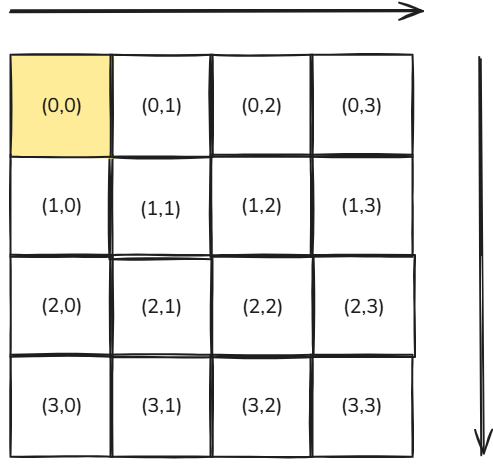
\includegraphics[width=0.5\textwidth]{img/percorre_grade.png}
    \caption{\small Percurso da grade 2D durante as iterações do autômato celular.}
    \label{fig:percorre_grade}
\end{figure}

A respeito da interação entre as células das bordas da malha, o modelo adota a condição de contorno \textbf{toroidal}, no qual as células da borda interagem com as células opostas. Por exemplo, uma célula que está na borda direita da malha está conectada à célula horizontalmente oposta, na borda esquerda da malha, e vice-versa. Da mesma forma, uma célula na borda superior da malha conecta-se verticalmente a uma na borda inferior e vice-versa. Uma célula localizada em uma aresta, portanto, interage tanto com sua vizinha oposta horizontal quanto com aquela na vertical. A Figura \ref{fig:torus} ilustra a condição de contorno toroidal aplicada ao modelo. Nota-se que a vizinhança de von Neumann da célula (0, 0) é composta pelas células (0, 1), (1, 0), (3, 0) e (0, 3).

\begin{figure}[H]
    \centering
    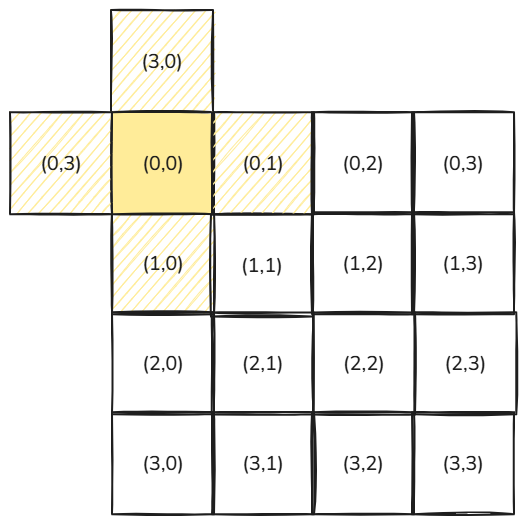
\includegraphics[width=0.5\textwidth]{img/torus.png}
    \caption{\small Condição de contorno toroidal aplicada ao modelo de autômato celular.}
    \label{fig:torus}
\end{figure}

A quantidade de células ocupadas por cada componente químico é definida por frações relativas, que representam a proporção de células ocupadas por cada tipo de componente em relação ao total de células de componentes da grade. Por exemplo, se a fração de células ocupadas por água for 0,6, isso significa que 60\% do total de componentes presentes na malha é composto por água, enquanto os 40\% restantes podem estar ocupados por outros componentes químicos.

Estabelece-se, também, uma fração de células vazias, que representa a proporção de células que não representam nenhum componente químico. Essa fração é igual a 31\% no modelo, o que significa que 31\% das células da grade estão vazias e não ocupadas por nenhum componente (ver \hyperref[subsubsec:fracao_celulas_vazias]{\textbf{Fração de Células Vazias}}). As frações de células ocupadas por cada componente químico são definidas como parâmetros do modelo e podem ser ajustadas conforme necessário para simular diferentes cenários, mas a fração de vazios é fixa.


\subsection{Regras de Evolução}

As regras de evolução do autômato celular são definidas por cinco parâmetros principais: \hyperref[subsubsec:Pm]{$P_M$}, \hyperref[subsubsec:Pb]{$P_B$}, \hyperref[subsubsec:J]{$J$}, \hyperref[subsubsec:Pr]{$P_R$} e \hyperref[subsubsec:Prot]{$P_{rot}$}. Cada um desses parâmetros desempenha um papel crucial na dinâmica do sistema, influenciando a movimentação dos componentes químicos, a formação de ligações, as reações químicas e a rotação dos componentes. A seguir, detalham-se as regras de evolução determinadas para o modelo:

\subsubsection{Movimentação dos Componentes Químicos}
\label{subsubsec:evolucao_movimentacao}

A movimentação básica dos componentes químicos na grade é regida pelo parâmetro probabilidade de movimentação livre (\hyperref[subsubsec:Pm]{$P_M$}). Durante cada iteração do autômato celular, cada célula com um componente químico tem uma probabilidade $P_M$ de se mover para uma célula vizinha vazia dentro de sua vizinhança de von Neumann. Dado que um componente A em estudo irá se mover, com chance indicada pelo valor de $P_M (A)$, a movimentação ocorre de forma aleatória, escolhendo uma das quatro células vizinhas de von Neumann (superior, inferior, esquerda ou direita) para a qual o componente pode se mover. Isso indica que a movimentação é estocástica e que $P_M (A)$ é o mesmo para qualquer vizinho vazio (Figura \ref{fig:evolucao_Pm}). Caso não haja células vizinhas vazias, o componente permanece em sua posição atual.

\begin{figure}[H]
    \centering
    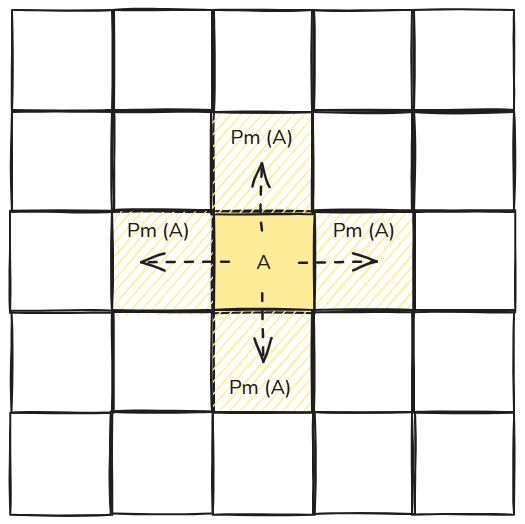
\includegraphics[width=0.5\textwidth]{img/evolucao_Pm.png}
    \caption{\small Exemplo de movimentação livre de um componente A para uma célula vazia da sua vizinhança de von Neumann.}
    \label{fig:evolucao_Pm}
\end{figure}

Frequentemente, um componente possui um ou mais componentes em sua vizinhança de von Neumann e/ou von Neumann estendida. Nesse caso, diferentes efeitos são combinados e, portanto, a movimentação do componente é influenciada por outros parâmetros, como a probabilidade de quebra de ligações (\hyperref[subsubsec:Pb]{$P_B$}) e a propensão de junção (\hyperref[subsubsec:J]{$J$}). A Figura \ref{fig:evolucao_Pm_Pb_J} ilustra um cenário da movimentação de um componente A, que possui um componente B em sua vizinhança de von Neumann e um componente C em sua vizinhança de von Neumann estendida. Nesse caso, a movimentação do componente A é influenciada pela probabilidade de quebra da interação $P_B (AB)$ e pela propensão de junção $J(AC)$, além de seu próprio $P_M (A)$.

\begin{figure}[H]
    \centering
    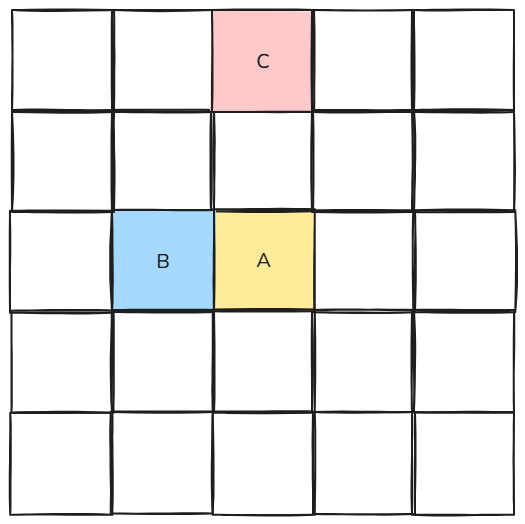
\includegraphics[width=0.5\textwidth]{img/evolucao_Pm_Pb_J.png}
    \caption{\small Cenário de evolução da movimentação de A, que deve considerar os parâmetros $P_M (A)$, $P_B (AB)$ e $J(AC)$.}
    \label{fig:evolucao_Pm_Pb_J}
\end{figure}

Dadas as propriedades básicas de probabilidade, a probabilidade total de movimentação de um componente $\alpha$ pode ser expressa como:

\begin{equation}
    \label{eq:pmov_total}
    P_\text{total}(\alpha) =
    \begin{cases}
        0,                                                                                            & \text{se } \left| V(\alpha) \right| = 4, \\[2ex]
        P_\text{M}(\alpha)\ \cdot \displaystyle\prod_{\beta \in V(\alpha)} P_\text{B}(\alpha, \beta), & \text{caso contrário}
    \end{cases}
\end{equation}

onde $P_\text{M}(\alpha)$ é a probabilidade de movimentação livre do componente $\alpha$, $V(\alpha)$ representa o conjunto de componentes vizinhos de von Neumann de $\alpha$, e $P_\text{B}(\alpha, \beta)$ é a probabilidade de quebra da interação entre $\alpha$ e cada vizinho $\beta$. Assim, a movimentação do componente $\alpha$ ocorre com probabilidade $P_\text{total}(\alpha)$, que depende tanto de sua mobilidade intrínseca quanto do produto das probabilidades de quebra das ligações com seus vizinhos imediatos. Caso todas as células vizinhas estejam ocupadas (ou seja, $\alpha$ possui quatro componentes vizinhos), o componente permanece em sua posição original.

No exemplo da Figura \ref{fig:evolucao_Pm_Pb_J}, portanto, a probabilidade do componente A se mover para uma célula vizinha vazia é dada por:
\begin{equation}
    P_\text{total}(A) = P_M(A) \cdot P_B(AB)
\end{equation}

Ainda nesse exemplo, a condição para que A se movimente é dada por $P_\text{total}(A)$, mas a direção do movimento é influenciada pelo parâmetro $J(AC)$, que determina a propensão de A se juntar a C. Define-se, portanto, que a célula vizinha vazia escolhida para o movimento de um componente genérico $\alpha$ será aquela que maximiza a propensão de junção de $\alpha$, ou seja, a célula vizinha vazia $v$ tal que:

\begin{equation}
    v^* = \underset{v \in \mathcal{V}_0(\alpha)}{\arg\max} \; J(\alpha, \beta_v), \quad \text{se } J(\alpha, \beta_v) \geq 1
\end{equation}

Isso significa que, se $\alpha$ tem múltiplas células vizinhas vazias adjacentes e dado que o movimento ocorrerá, a célula escolhida para o movimento será aquela na direção da maior propensão de junção de $\alpha$ com um dos componentes da sua vizinhança externa. A vizinhança externa $\mathcal{V}_\text{ext}(v)$ de um componente é definida pelas 4 células mais distantes dentro da sua vizinhança de von Neumann estendida.

Ao assumir valores entre 0 e 1, o parâmetro $J$ revela repulsão entre componentes. Logo, define-se que a movimentação de um componente na direção de outro é permitida apenas se $J(\alpha, \beta) \geq 1$, ou seja, se a propensão de junção for maior ou igual a 1. Caso contrário, o componente $\alpha$ não se movimenta na direção de $\beta$. Células vazias da vizinhança externa são consideradas neutras, ou seja, elas são preteridas em junção caso haja qualquer outra célula com $J(\alpha, \beta) \geq 1$ e serão favorecidas se $0 < J(\alpha, \beta) < 1$ para todas as células vizinhas externas. O modelo, especialmente no lado computacional, interpreta células vazias com $J = 0$.

No exemplo da Figura \ref{fig:evolucao_Pm_Pb_J}, se A se mover e $J(AC) \geq 1$, a célula escolhida será aquela que maximiza $J$, ou seja, a célula vizinha vazia mais próxima de C. Caso contrário, se $0 < J(AC) < 1$, A não se movimenta na direção de C devido à repulsão, e a célula escolhida poderá ser aleatoriamente qualquer das outras células vizinhas vazias em que não há componentes na vizinhança externa ($J = 0$). A Figura \ref{fig:evolucao_A} ilustra as diferentes possibilidades de movimentação de A.

\begin{figure}[H]
    \centering
    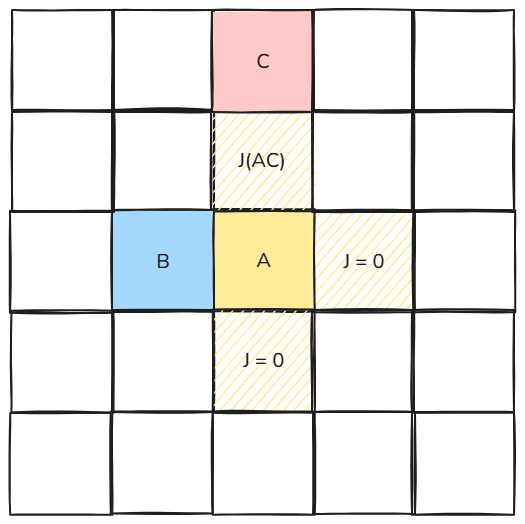
\includegraphics[width=0.5\textwidth]{img/evolucao_A.png}
    \caption{\small Possibilidades de movimentação do componente A. Se $J(AC) \geq 1$, A se movimenta na direção de C (para cima). Se $0 < J(AC) < 1$, A se movimenta para a direita ou para baixo.}
    \label{fig:evolucao_A}
\end{figure}

Há uma relação conceitual importante entre a propensão de junção $J$ e a probabilidade de quebra de ligação $P_B$. Levando em consideração aspectos de atração/repulsão e interações intermoleculares, é natural imaginar que quanto maior a propensão de junção entre dois componentes, menor será a probabilidade de quebra da ligação entre eles e vice-versa. Assim, propõe-se para o modelo uma relação matemática entre $J$ e $P_B$, dada por:

\begin{equation}
    \label{eq:J_PB}
    P_B(\alpha, \beta) = \frac{1.5}{J(\alpha, \beta) + 1.5}, \quad (\alpha, \beta \in \mathcal{C})
\end{equation}
onde $\alpha$ e $\beta$ representam componentes do sistema, $P_B(\alpha, \beta)$ é a probabilidade de quebra da ligação entre os componentes $\alpha$ e $\beta$, e $J(\alpha, \beta)$ é a propensão de junção entre eles. Quando $J(\alpha, \beta) = 0$, temos $P_B(\alpha, \beta) = 1$, indicando que não há propensão de junção e a ligação é sempre quebrada. Por outro lado, quando $J(\alpha, \beta) \to \infty$, temos $P_B(\alpha, \beta) \to 0$, indicando que a ligação é sempre mantida.

Essa definição traz a vantagem de reduzir a quantidade de parâmetros obrigatórios solicitados ao usuário do software, uma vez que basta definir as entradas de $J$ que os valores de $P_B$ poderão ser calculados automaticamente. A constante $1.5$ é um refinamento aplicado a fim de tanto obter probabilidades de quebra um pouco maiores, o que auxilia no aumento da dinâmica do sistema, quanto suavizar a variação de $P_B$ frente a mudanças em $J$, especialmente na região do domínio onde $J$ é maior porém próximo de 1, o que facilita o controle sobre as alterações que esses parâmetros causam no sistema.

\subsubsection{Reação e Rotação dos Componentes}

A fim de simular reações de cinética enzimática, em especial pelo mecanismo de Michaelis-Menten, o modelo trata melhor reações do tipo $E + S \rightleftharpoons ES \rightarrow E + P$, onde $E$ representa a enzima, $S$ o substrato, $ES$ o complexo enzima-substrato e $P$ o produto formado. Independentemente dos identificadores dos componentes, a reação básica mencionada é aquela estabelecida como a principal que o modelo é especializado em simular. As reações são regidas por parâmetros $P_R$, que podem tanto representar reações diretas quanto inversas.

O parâmetro $P_{rot}$ é utilizado para controlar a rotação de um dos componentes do sistema e também determina a possibilidade de atribuir diferentes comportamentos ao mesmo componente dependendo da direção de sua orientação. Essa característica é especialmente útil para simular o comportamento de surfactantes no sistema de cinética enzimática, visto que uma molécula de surfactante é conhecida por possuir um lado polar e uma cauda apolar. Uma combinação de parâmetros $J$, portanto, pode ser utilizada para simular uma dinâmica de atração do lado polar por espécies químicas polares, bem como a atração da cauda apolar por espécies apolares.

Dado que uma rotação irá ocorrer, a próxima orientação do componente rotacionável será aleatória, não dependendo de outros fatores ou parâmetros. Além disso, a rotação de um componente poderá ocorrer somente se não houver nenhum outro componente em sua vizinhança de von Neumann. Isso evita que a rotação cause quebras indesejadas de interações já estabelecidas por outros parâmetros e garante que as responsabilidades de movimentação/interação e rotação sejam bem definidas.

\section{Implementação Computacional}

\subsection{Código Fonte do Modelo}

O modelo de autômato celular foi implementado em Python utilizando a biblioteca \textit{NumPy} (\citetitle{numpy}) para manipulação de arrays e matrizes. O código fonte está disponível no repositório do GitHub \textbf{\citetitle{repositorio_tcc_eng_quimica}}, onde também estão documentadas as instruções de execução. Essa linguagem foi escolhida pela sua simplicidade e pela vasta gama de bibliotecas disponíveis para manipulação de dados e visualização, facilitando o desenvolvimento e a análise dos resultados, bem como a leitura e entendimento do código, visto que Python é uma das linguagens mais utilizadas e conhecidas atualmente.

Além do cálculo de autômatos celulares, o código também inclui gerenciamento dos dados das simulações, como o recebimento e o tratamento das entradas do usuário, a busca desses dados a qualquer momento e a exportação dos resultados para arquivos CSV. Para lidar com tudo isso, foi desenvolvida uma Web API utilizando a biblioteca \textit{Fastapi} (\citetitle{fastapi}), que permite a interação com o modelo por meio de requisições HTTP. Essa API facilita a integração do modelo com outras aplicações e, caso a aplicação seja implantada em um servidor, possibilita a execução de simulações de forma remota, tornando o modelo mais acessível e flexível para diferentes usuários.

O salvamento dos dados de entrada de simulações, bem como das malhas resultantes da execução das iterações, e outros dados relevantes, é feito em banco de dados SQL, como o PostgreSQL (\citetitle{postgresql}). Essa escolha permite uma gestão moderna e eficiente dos dados em detrimento do simples salvamento em arquivos, possibilitando consultas rápidas e a manutenção de um histórico de simulações consistente. A biblioteca \textit{SQLAlchemy} (\citetitle{sqlalchemy}) é utilizada para facilitar a interação com o banco de dados, permitindo a criação, leitura, atualização e exclusão de registros de forma simples e intuitiva.

Há, ainda, um processo de escrita de logs para registrar as atividades do modelo, como o início e o término de simulações, erros e avisos. Esses logs são armazenados em arquivos de texto, permitindo uma análise posterior do comportamento do modelo e facilitando a identificação de problemas ou otimizações necessárias.

O código do AC propriamente dito segue uma estrutura modular, onde as principais funções são responsáveis por inicializar a grade, aplicar as regras de movimentação, reação e rotação, e atualizar o estado do sistema a cada iteração. A seguir, apresenta-se um fluxograma simplificado do processo de simulação:

\begin{figure}[H]
    \centering
    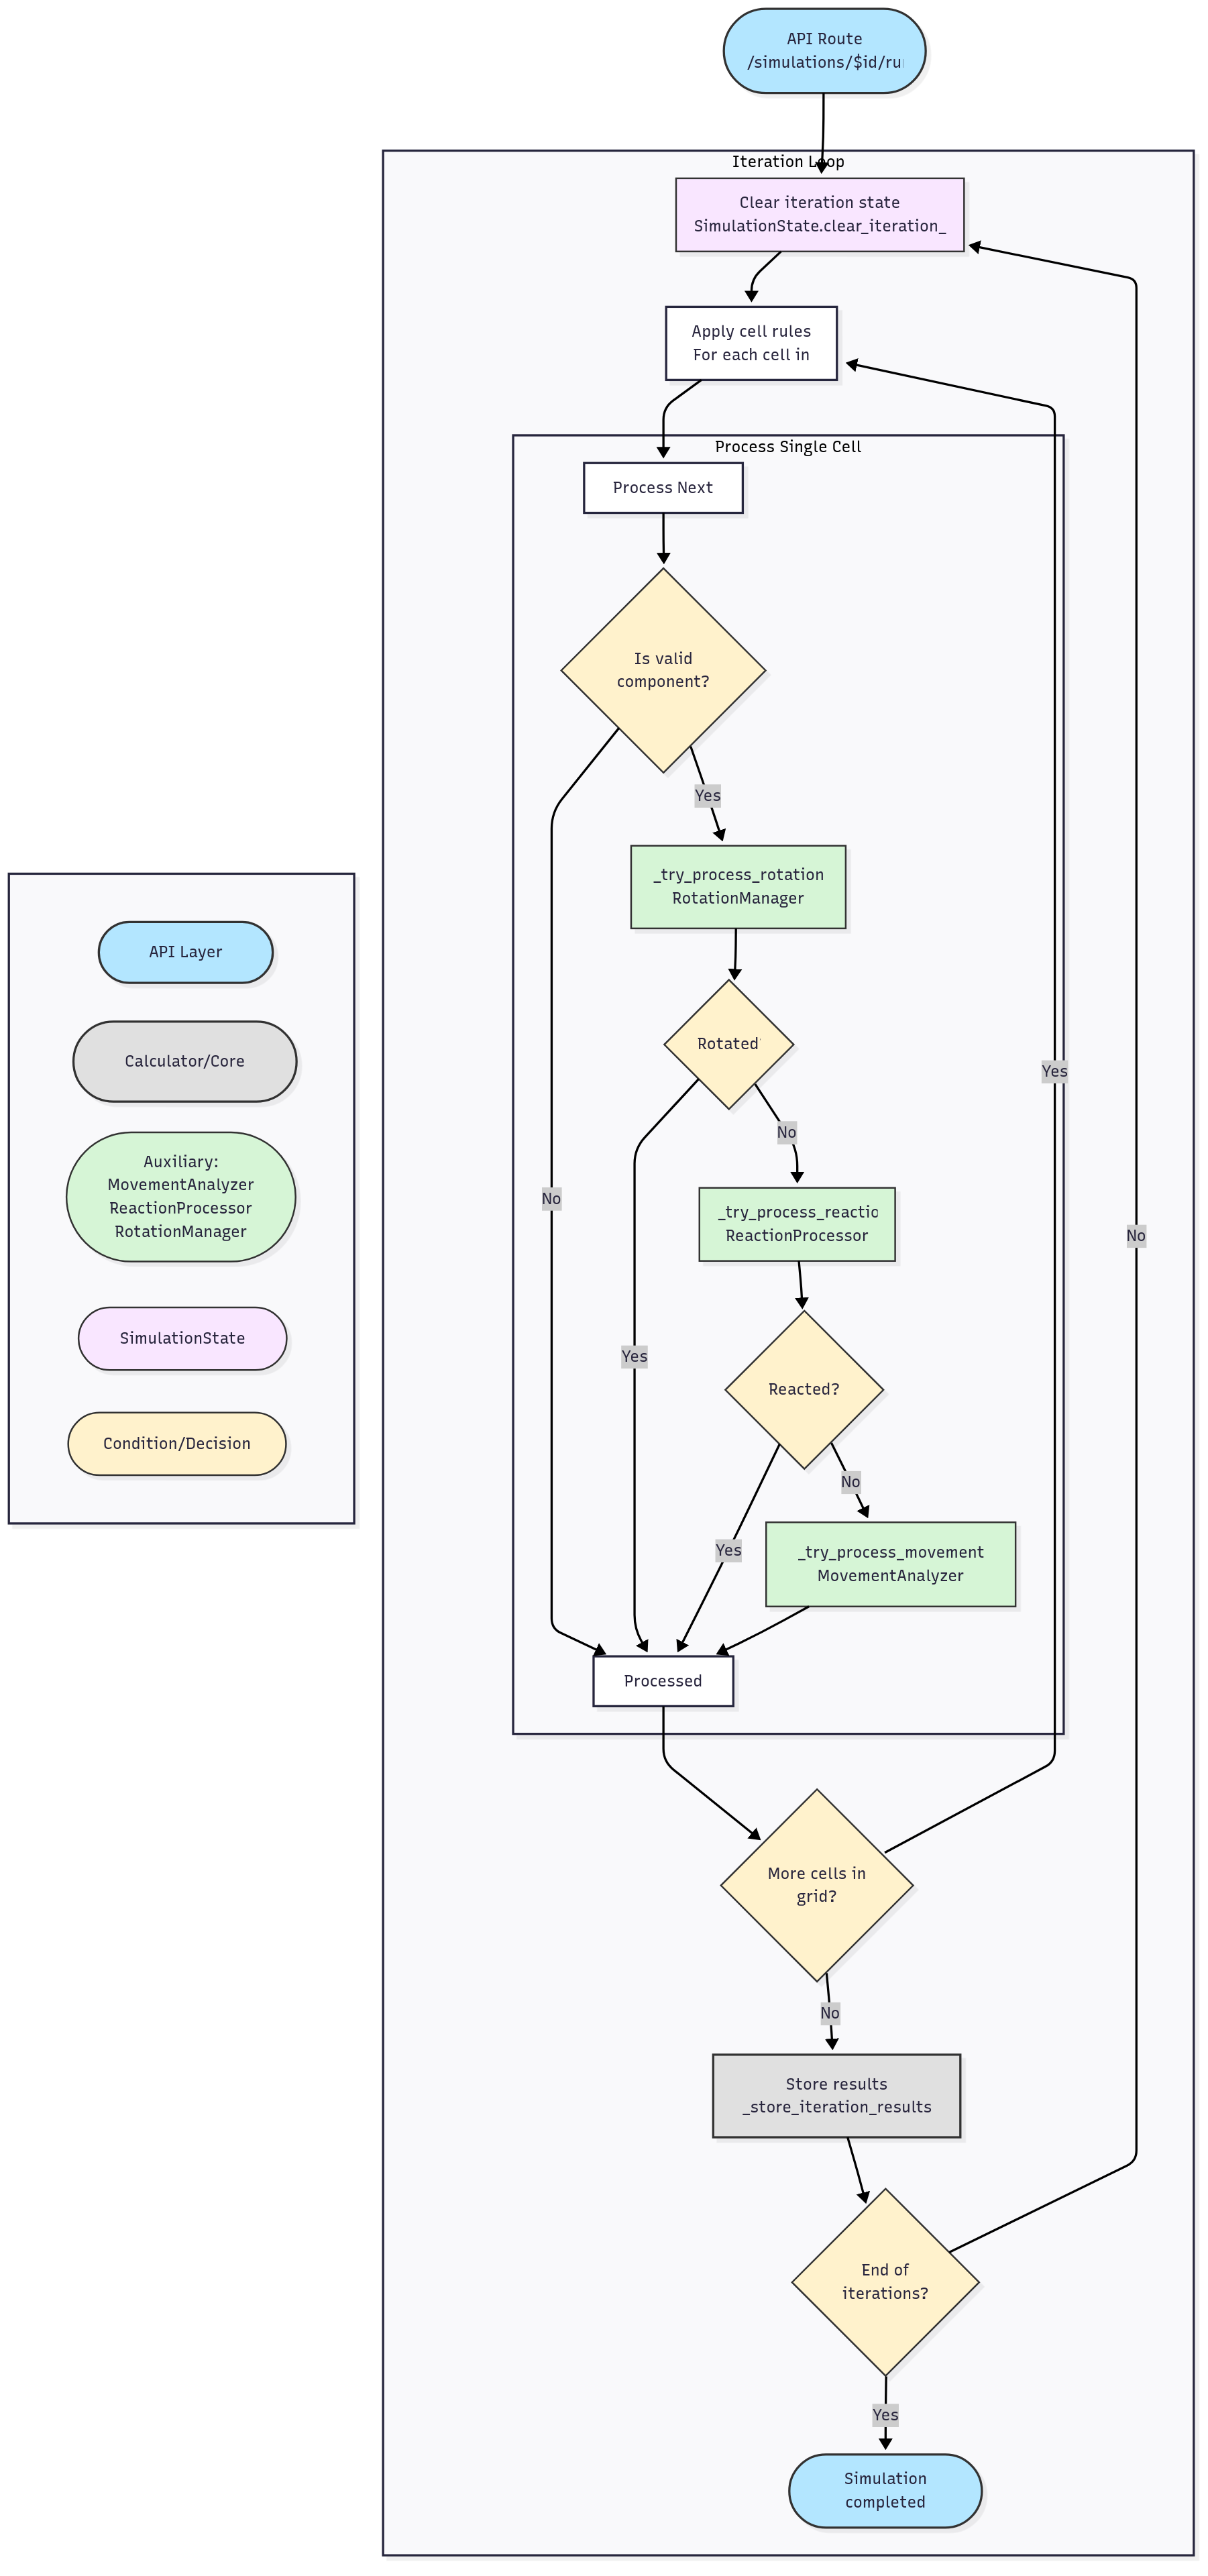
\includegraphics[width=0.7\textwidth]{img/fluxograma.png}
    \caption{Fluxograma do modelo de autômato celular implementado.}
    \label{fig:fluxograma}
\end{figure}

Pelo fluxograma, nota-se que a execução de uma simulação do modelo de autômato celular é iniciada com a requisição para uma rota da API, recebendo como parâmetro o identificador único da simulação previamente criada. Após, é instanciado um objeto da classe \textbf{CellularAutomataCalculator}, que é responsável por gerenciar a simulação. É chamado o método \textbf{calculate\_cellular\_automata()} desse objeto, que inicia o processo de simulação. O método \textbf{initialize\_simulation()} é chamado para inicializar a grade e os componentes químicos com um estado inicial aleatório, de acordo com as frações relativas definidas pelo usuário. É instanciado um objeto da classe \textbf{SimulationState}, responsável por guardar alguns estados entre iterações, como as células com componentes que foram movidos e os que reagiram. Esses estados são devidamente limpos e, então, o processo iterativo se inicia.

Durante cada iteração, a malha é percorrida célula por célula, seguindo a ordem de leitura já estabelecida, isto é, da esquerda para a direita e de cima para baixo. Para cada célula, são aplicadas as regras de movimentação, reação e rotação, conforme os parâmetros definidos. Observando o fluxograma, o processamento de uma célula inicia com a verificação se a célula está vazia ou não. Se estiver vazia, o processo é encerrado para aquela célula e a próxima célula é processada. Caso contrário, o modelo tenta primeiramente rotacionar o componente atual, por meio de uma classe responsável chamada \textbf{RotationManager}, caso seja um componente rotacionável. Se a rotação for bem-sucedida, o componente é atualizado e o processo para aquela célula é encerrado. Se não for possível rotacionar, o modelo tenta reagir o componente com um de seus vizinhos, considerando as regras de reação e os parâmetros $P_R$, por meio da classe \textbf{ReactionProcessor}. Se a reação for bem-sucedida, os componentes envolvidos nela são atualizados e o processo para aquela célula é encerrado. Caso contrário, o modelo tenta movimentar o componente para uma célula vizinha vazia, considerando as regras de movimentação e os parâmetros $P_M$ e $P_B$, por meio da classe \textbf{MovementAnalyzer}. Se a movimentação for bem-sucedida, o componente é atualizado e o processo para aquela célula é encerrado. Se nenhuma das ações for possível, o componente permanece em sua posição atual e o fluxo também é encerrado.

Depois de toda essa análise, o programa passa para a próxima célula caso haja alguma célula não processada na grade e repete o fluxo de aplicação das regras até que todas as células da grade tenham sido processadas. Nesse ponto, uma iteração na malha é concluída e o resultado é salvo em memória. Caso o número de iterações definido pelo usuário ainda não tenha sido atingido, uma nova iteração se inicia a partir da malha gerada pela iteração anterior, limpando apenas as informações de células onde houve movimentação ou reação, por exemplo. Quando todas as iterações são concluídas, a simulação é finalizada e os resultados são salvos no banco de dados para posterior consulta e análise. Vale ressaltar que o estado de cada malha após todas as iterações é salvo, isto é, o usuário é capaz de consultar a exata malha resultante de qualquer iteração específica, o que permite uma análise visual do comportamento do sistema ao longo do tempo.

Para garantir a confiabilidade do modelo, foram implementados testes unitários utilizando a biblioteca \textit{pytest} do Python. Esses testes cobrem algumas das principais funcionalidades do modelo, como a movimentação, reação e rotação dos componentes, bem como a inicialização da grade e o processamento das iterações. Esses testes podem ser executados como forma de validar que o modelo está funcionando corretamente e que as regras de evolução estão sendo aplicadas conforme o esperado.

A Figura \ref{fig:unit_tests} ilustra o resultado da execução dos testes unitários, onde todos os testes foram aprovados, indicando que as regras implementadas foram testadas e estão retornando os resultados esperados. São, ao todo, 60 testes unitários, executados com o comando \texttt{pytest -v} e todos estão aprovados, conforme a saída apresentada na figura.

\begin{figure}[H]
    \centering
    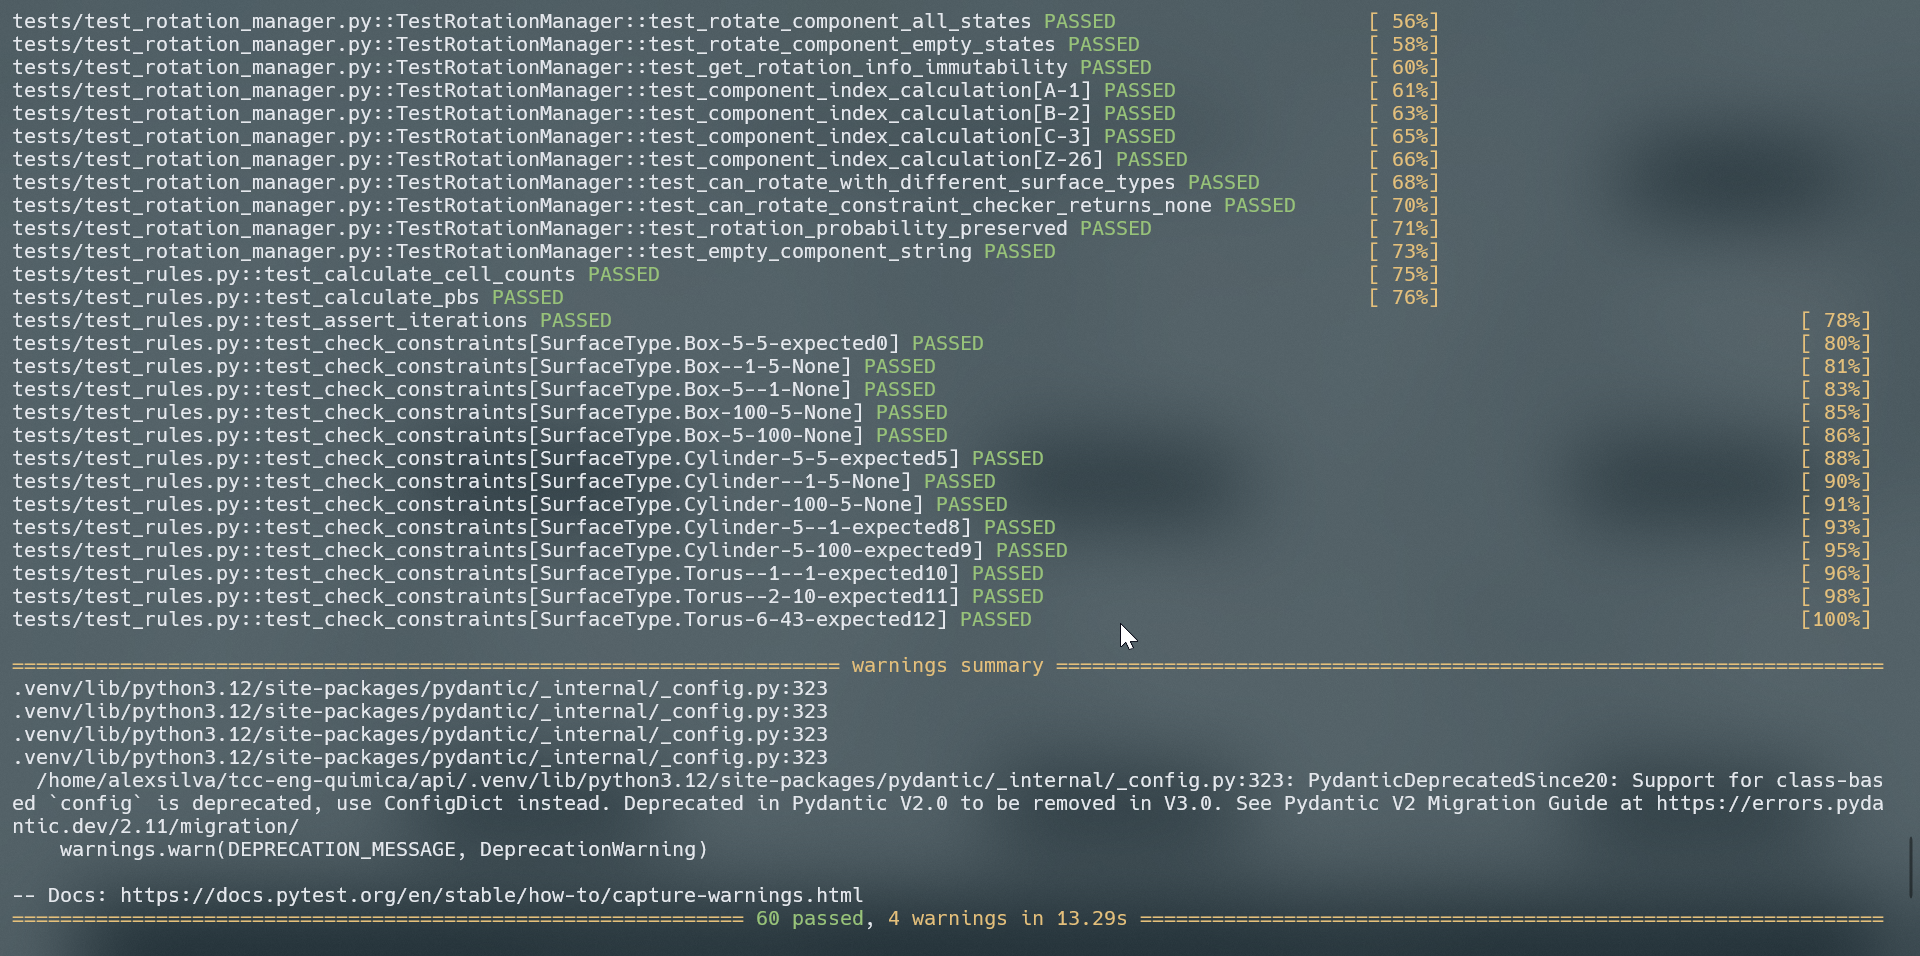
\includegraphics[width=1\textwidth]{img/unit_test.png}
    \caption{\small Resultado da execução dos testes unitários do modelo de autômato celular.}
    \label{fig:unit_tests}
\end{figure}

\subsection{Interface do Usuário}

O software deste trabalho tem um foco grande em tornar a experiência do usuário a mais simples possível, permitindo que usuários com pouca ou nenhuma experiência em programação consigam executar simulações de autômatos celulares e analisar os resultados. Para isso, foi desenvolvida uma interface gráfica amigável, utilizando a biblioteca especializada na construção de interfaces gráficas executadas em navegadores web, o \textit{React} (\citetitle{react}).

A interface, portanto, foi projetada para ser executada em um navegador web, permitindo que o usuário interaja com o modelo de autômato celular por meio de uma aplicação web. Dessa forma, o usuário pode utilizar as ferramentas do software em um ambiente bastante familiar.

Assim que a aplicação é iniciada, o usuário é apresentado à tela inicial da Figura \ref{fig:interface_inicial}, onde pode criar uma nova simulação ou acessar simulações já existentes. Há um botão em destaque no canto superior direito para dar início a uma nova simulação. Simulações já existentes são visualizadas nessa tela com algumas informações básicas, como o nome, o número de iterações e o tamanho da grade. O usuário pode abrir, editar, excluir ou criar uma cópia de uma simulação salva.

\begin{figure}[H]
    \centering
    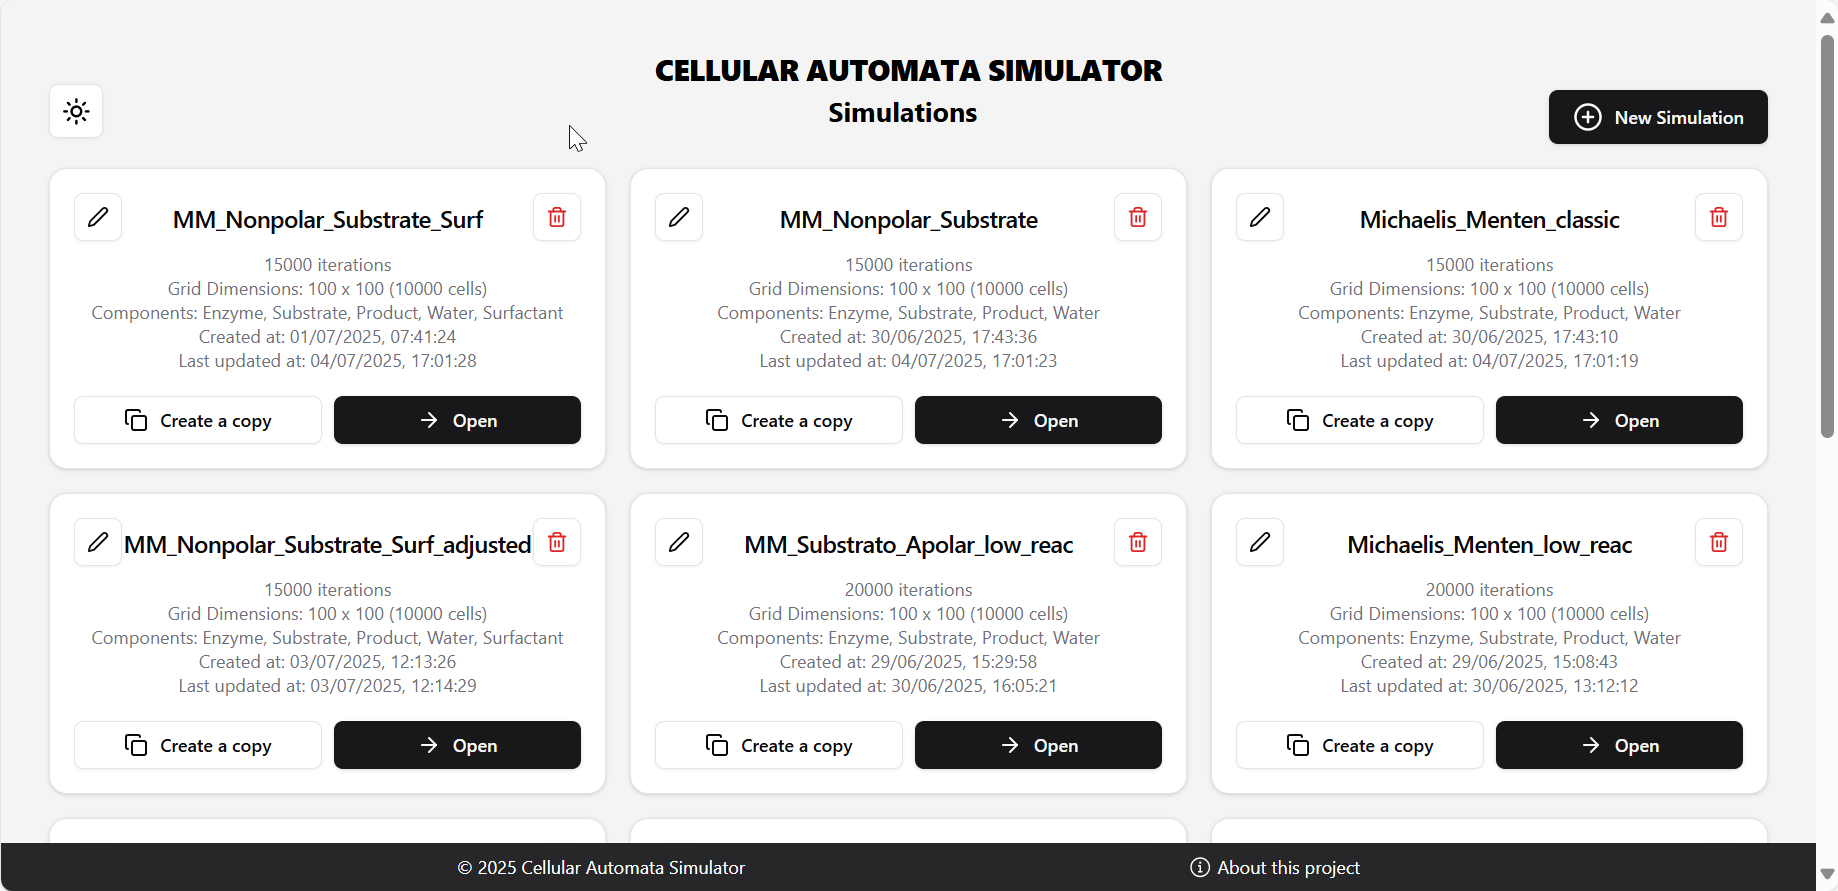
\includegraphics[width=1\textwidth]{img/interface_inicial.png}
    \caption{\small Tela inicial da interface do usuário do simulador de autômatos celulares.}
    \label{fig:interface_inicial}
\end{figure}

Ao criar uma nova simulação do início, o usuário é direcionado para um formulário de configuração conforme as Figuras \ref{fig:interface_configuracao1} e \ref{fig:interface_configuracao2}, onde pode definir o nome da simulação, o tamanho da grade (número de células na horizontal e vertical), o número de iterações, as frações relativas de cada componente químico, a probabilidade de movimentação livre, a probabilidade de quebra de ligações, a propensão de junção e a probabilidade de reação. O usuário também pode escolher se deseja ativar ou não a rotação de um dos componentes e inserir uma probabilidade de rotação.

\begin{figure}[H]
    \centering
    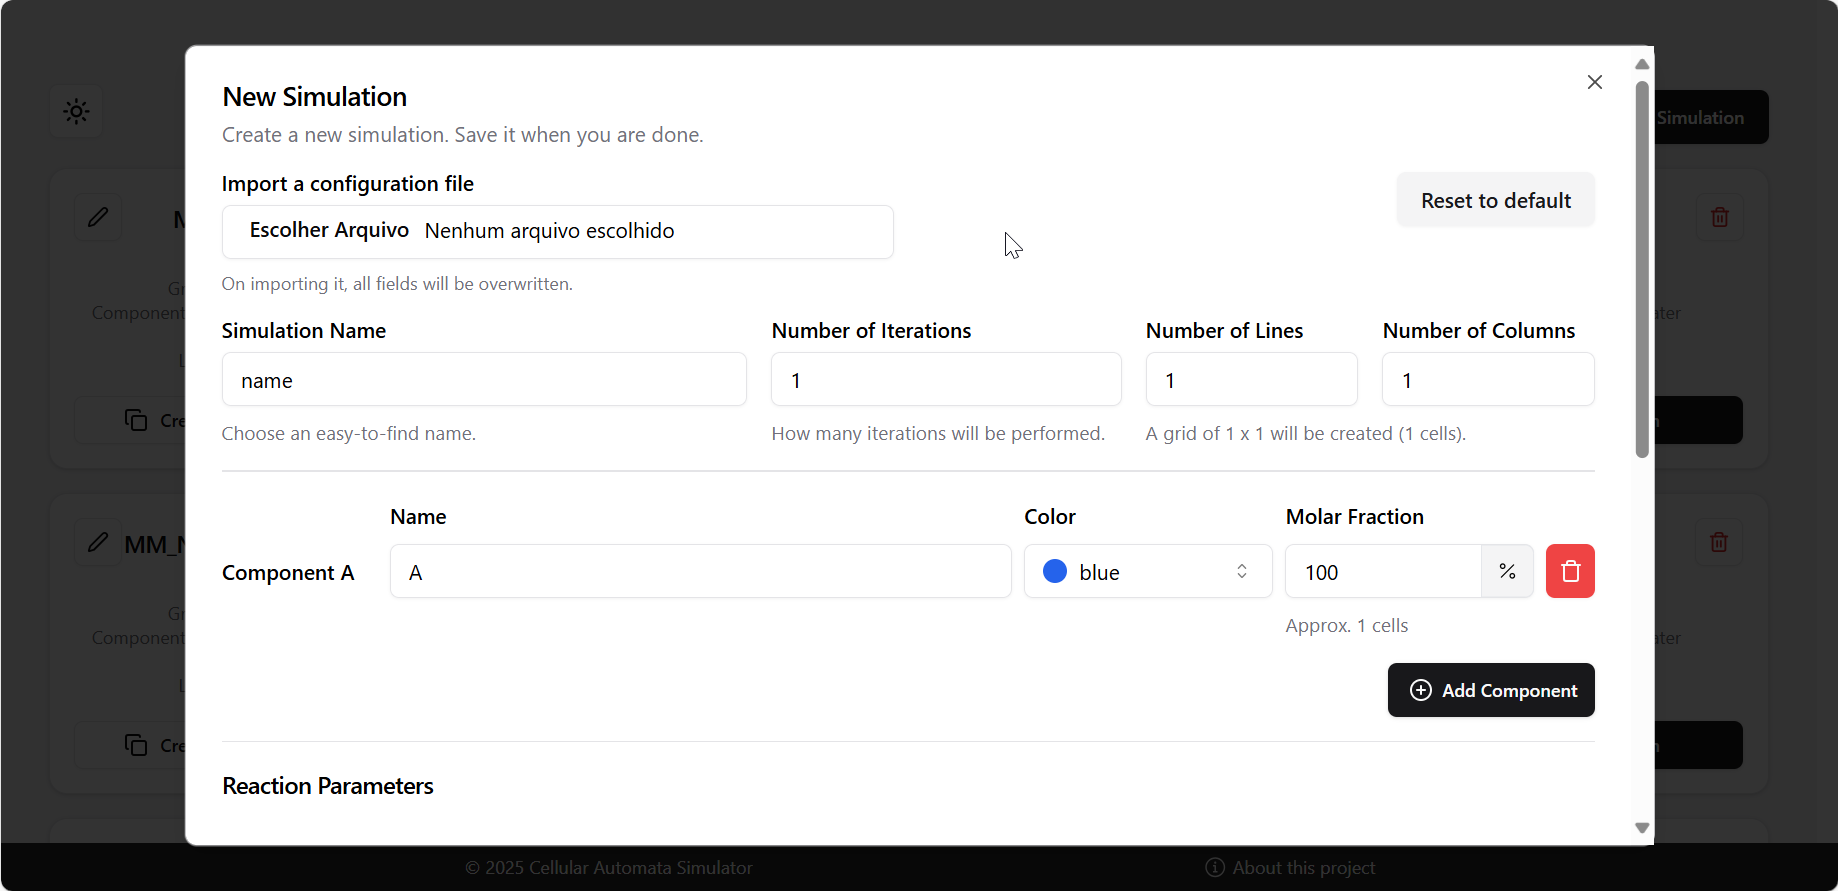
\includegraphics[width=1\textwidth]{img/interface_configuracao.png}
    \caption{\small Primeira parte do formulário de configuração de uma nova simulação.}
    \label{fig:interface_configuracao1}
\end{figure}

\begin{figure}[H]
    \centering
    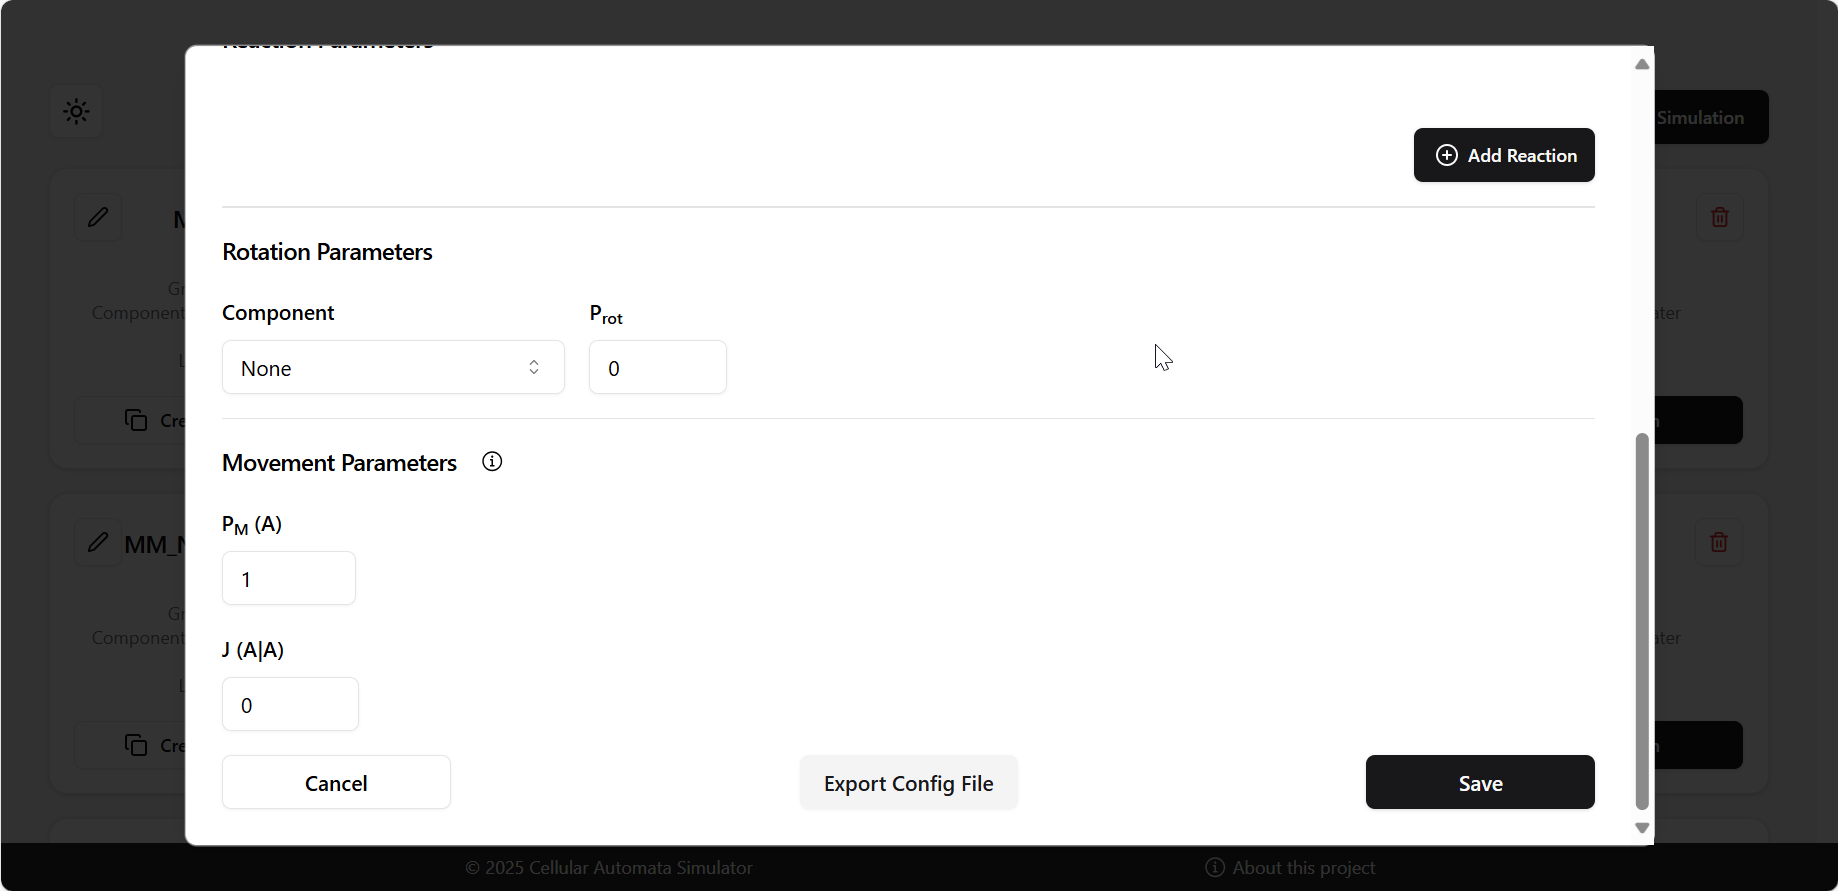
\includegraphics[width=1\textwidth]{img/interface_configuracao2.png}
    \caption{\small Segunda parte do formulário de configuração de uma nova simulação.}
    \label{fig:interface_configuracao2}
\end{figure}

O formulário é intuitivo e possui diversas validações para garantir que os dados inseridos pelo usuário sejam consistentes. Por exemplo, o tamanho da grade deve ser um número inteiro positivo, o número de iterações deve ser um inteiro positivo, as frações relativas devem somar 1, e as probabilidades devem estar entre 0 e 1. Os parâmetros $J$ aceitam valores positivos. Caso o usuário insira dados inválidos, mensagens de erro são exibidas para orientá-lo a corrigir os valores. A Figura \ref{fig:validacao} ilustra um exemplo de erro de validação, onde o usuário está inserindo uma fração relativa de 50\% mas há somente um componente naquele momento e a soma das frações relativas deve ser igual a 100\%.

\begin{figure}[H]
    \centering
    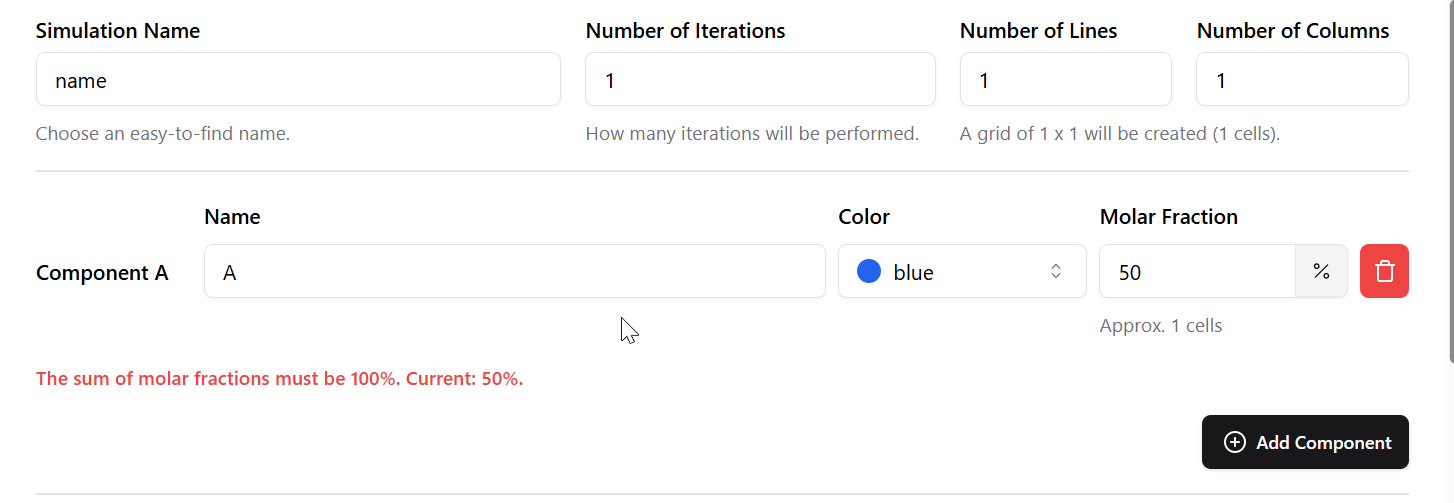
\includegraphics[width=1\textwidth]{img/validacao.png}
    \caption{\small Exemplo de erro de validação ao tentar inserir uma fração relativa inválida.}
    \label{fig:validacao}
\end{figure}

Outra informação que pode auxiliar o usuário a entender melhor o que está sendo inserido é a quantidade de células total que serão geradas de acordo com o tamanho da grade e a quantidade aproximada de células que serão ocupadas por cada componente. Essas informações são atualizadas dinamicamente conforme o usuário preenche os campos do formulário, permitindo que ele tenha uma visão clara do que está configurando. A Figura \ref{fig:informacoes} ilustra essas informações adicionais. Note que já são mostradas a quantidade total de células na grade (10000 células) e a quantidade aproximada de células ocupadas por cada componente, considerando as frações relativas inseridas pelo usuário.

Os valores de células ocupadas são aproximados pois o número total de células é fixo, mas as frações relativas podem não ser inteiras. Além disso, a fração de células vazias é sempre 31\% do total e a aplicação já calcula a quantidade correta de componentes e vazios automaticamente, considerando que as frações são calculadas sobre a quantidade total de células \textbf{ocupadas}.

\begin{figure}[H]
    \centering
    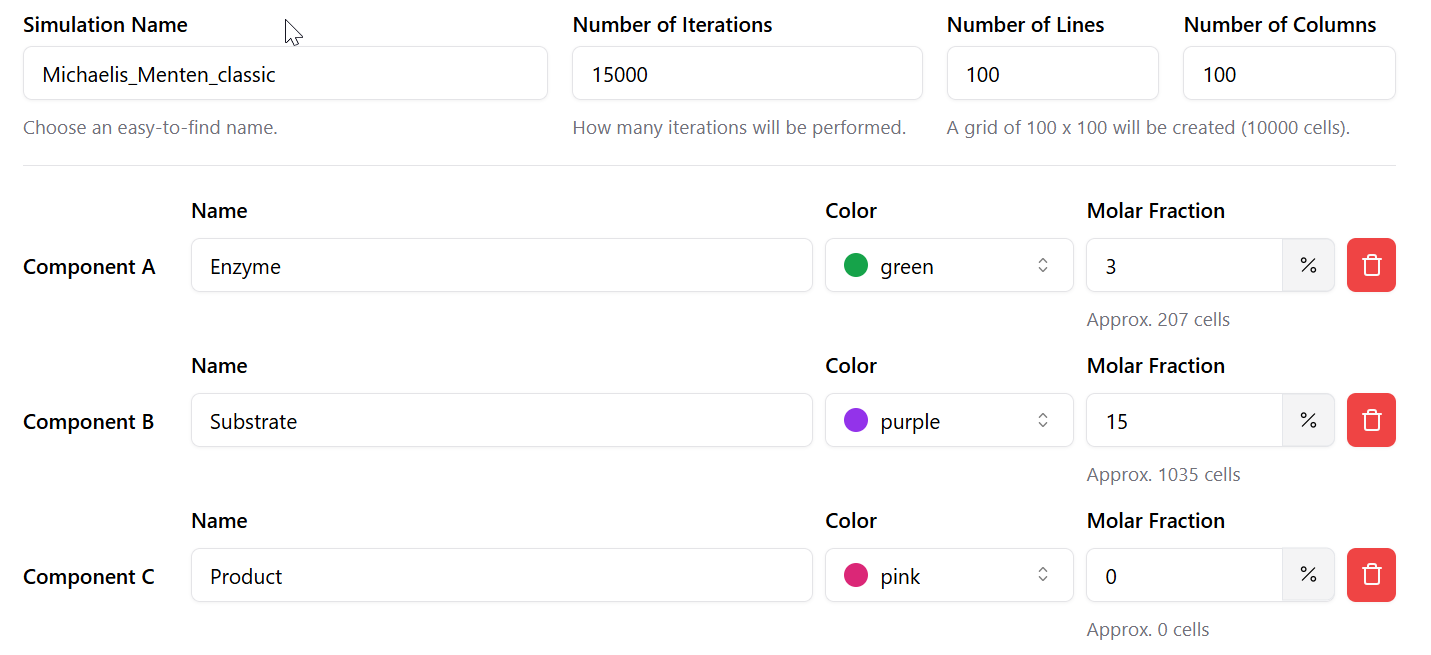
\includegraphics[width=1\textwidth]{img/calculo_celulas.png}
    \caption{\small Informações adicionais sobre a simulação, como o número total de células e a quantidade aproximada de células ocupadas por cada componente.}
    \label{fig:informacoes}
\end{figure}

Após a configuração básica e das frações, o usuário pode adicionar uma reação e configurá-la. A Figura \ref{fig:interface_reacao} ilustra os dados de uma reação já configurada para o cálculo de cinética enzimática. Note a configuração dos componentes envolvidos e as probabilidades de reação direta e inversa.

\begin{figure}[H]
    \centering
    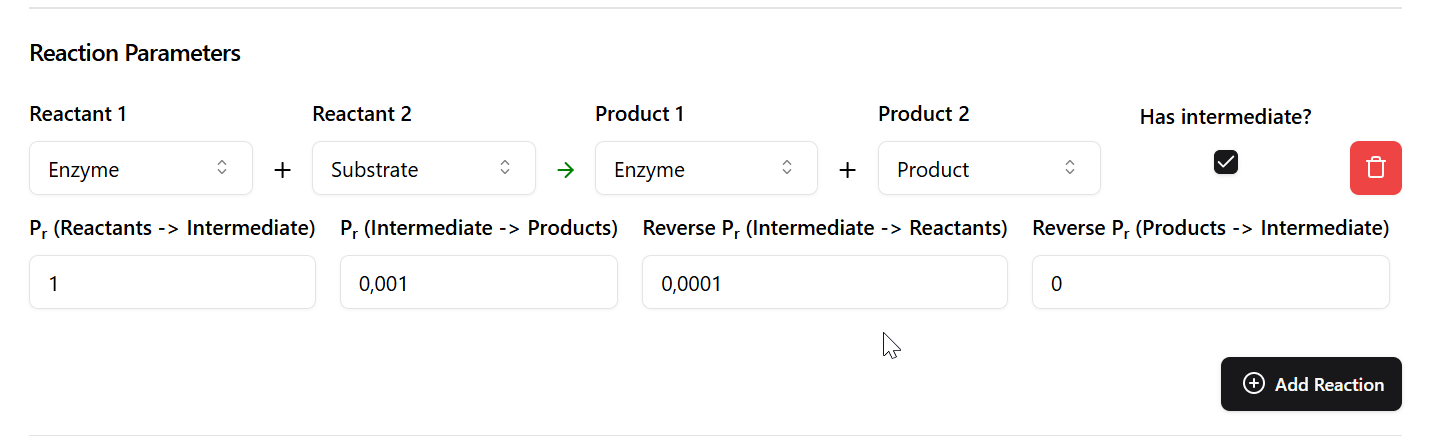
\includegraphics[width=1\textwidth]{img/reacao_config.png}
    \caption{\small Configuração de uma reação no formulário de configuração da simulação.}
    \label{fig:interface_reacao}
\end{figure}

A possibilidade de adicionar um componente rotacionável é apresentada na seção de parâmetros de rotação, ilustada na Figura \ref{fig:interface_rotacao}. O usuário escolhe um dos componentes já cadastrados para ser rotacionável e define a probabilidade de rotação. A rotação é uma característica opcional, mas pode ser ativada para simular comportamentos específicos de componentes químicos, como surfactantes.

\begin{figure}[H]
    \centering
    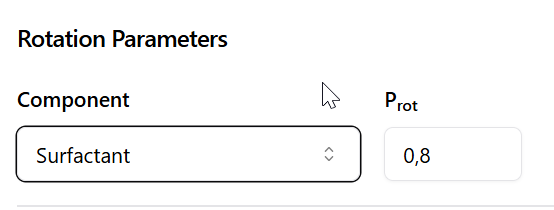
\includegraphics[width=0.5\textwidth]{img/rotacao_config.png}
    \caption{\small Configuração de um componente rotacionável no formulário de configuração da simulação.}
    \label{fig:interface_rotacao}
\end{figure}

Logo abaixo no formulário começa a configuração da movimentação, onde são definidos $P_M$ e $J$ para cada componente previamente inserido. Note que o software já fornece dinamicamente os campos necessários para a configuração de cada parâmetro de cada componente. Os componentes são identificados de forma genérica por uma letra em ordem alfabética, como A, B, C, etc., e é possível conferir a qualquer momento qual letra corresponde a qual componente através do elemento de informação, geralmente chamado de \textit{tooltip}, que aparece ao passar o mouse sobre o ícone \textit{i}.

\begin{figure}[H]
    \centering
    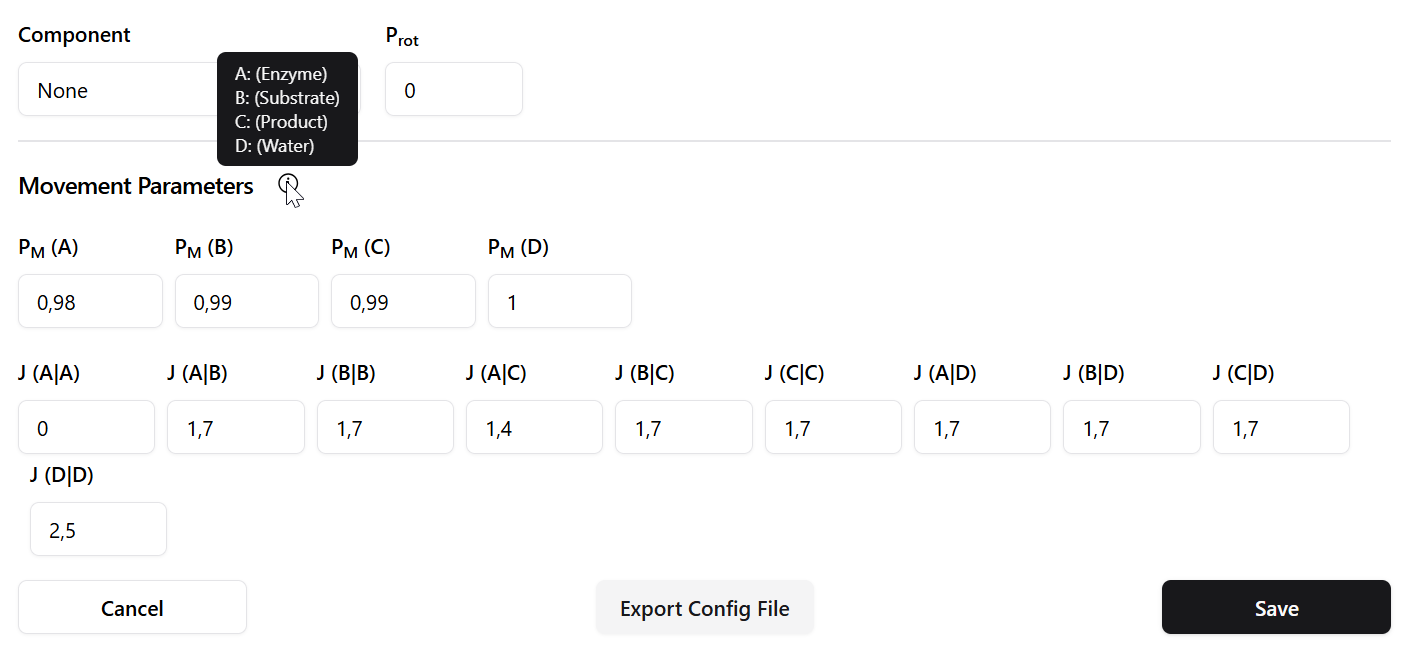
\includegraphics[width=1\textwidth]{img/mov_config.png}
    \caption{\small Configuração dos parâmetros de movimentação e propensão de junção no formulário de configuração da simulação.}
    \label{fig:interface_movimentacao}
\end{figure}

A fim de facilitar a criação de simulações, o software permite que o usuário baixe e importe arquivos de configuração pré-definidos, que contêm todos os parâmetros necessários para uma simulação. Esses arquivos são salvos no formato \textit{JSON} e podem ser facilmente editados em qualquer editor de texto. A Figura \ref{fig:interface_movimentacao} mostra o botão \textbf{Export Config File} para exportar esse arquivo a partir de uma simulação já preenchida e a Figura \ref{fig:interface_configuracao1} mostra o botão \textbf{Escolher Arquivo} para opcionalmente importar um arquivo de configuração previamente baixado. Isso permite que o usuário crie simulações complexas rapidamente, reutilizando configurações já testadas e validadas, ou ainda transfira esse arquivo para outro usuário poder importar em seu computador e executar a mesma simulação, sem a necessidade de preencher todos os campos manualmente.

Preenchidos e validados todos os dados obrigatórios, o usuário pode salvar a simulação pelo botão \textbf{Save} no canto inferior direito do formulário. Após salvar, o usuário é redirecionado para a tela inicial, onde a nova simulação já aparece na lista de simulações disponíveis.

Ao abrir uma simulação da lista de simulações existentes, o usuário é direcionado para a área de visualização da simulação. Caso ela não tenha sido executada ainda, é mostrada uma mensagem informando que a simulação ainda não foi executada e o usuário pode iniciar a execução clicando no botão \textbf{Run Simulation}. A Figura \ref{fig:interface_simulacao} ilustra essa tela de visualização de uma simulação ainda não executada.

\begin{figure}[H]
    \centering
    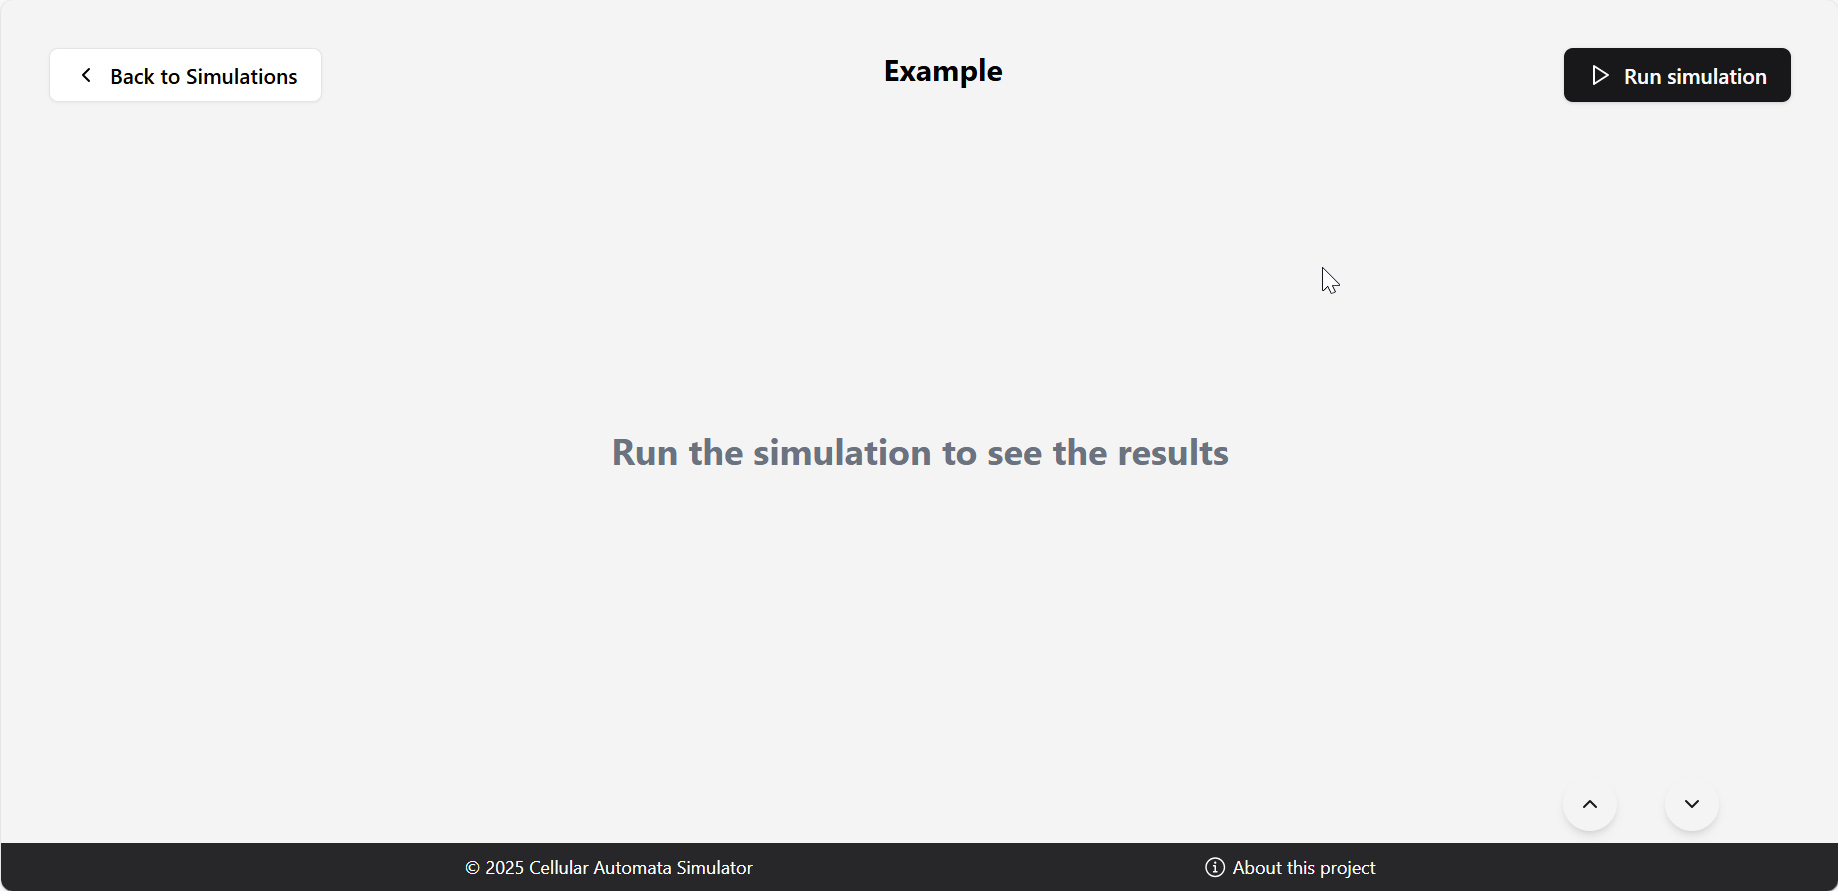
\includegraphics[width=1\textwidth]{img/empty_simulacao.png}
    \caption{\small Tela de visualização de uma simulação ainda não executada.}
    \label{fig:interface_simulacao}
\end{figure}

Ao executar a simulação, o usuário recebe informações sobre o progresso da execução em termos de porcentagem no canto superior direito. Nesse momento, o usuário pode realizar outras tarefas no computador que a simulação continuará sendo executada e terminará após atingir 100\% de progresso, salvando e exibindo resultados atualizados automaticamente. A Figura \ref{fig:interface_simulacao_executando} ilustra a mensagem de progresso de uma simulação em execução.

\begin{figure}[H]
    \centering
    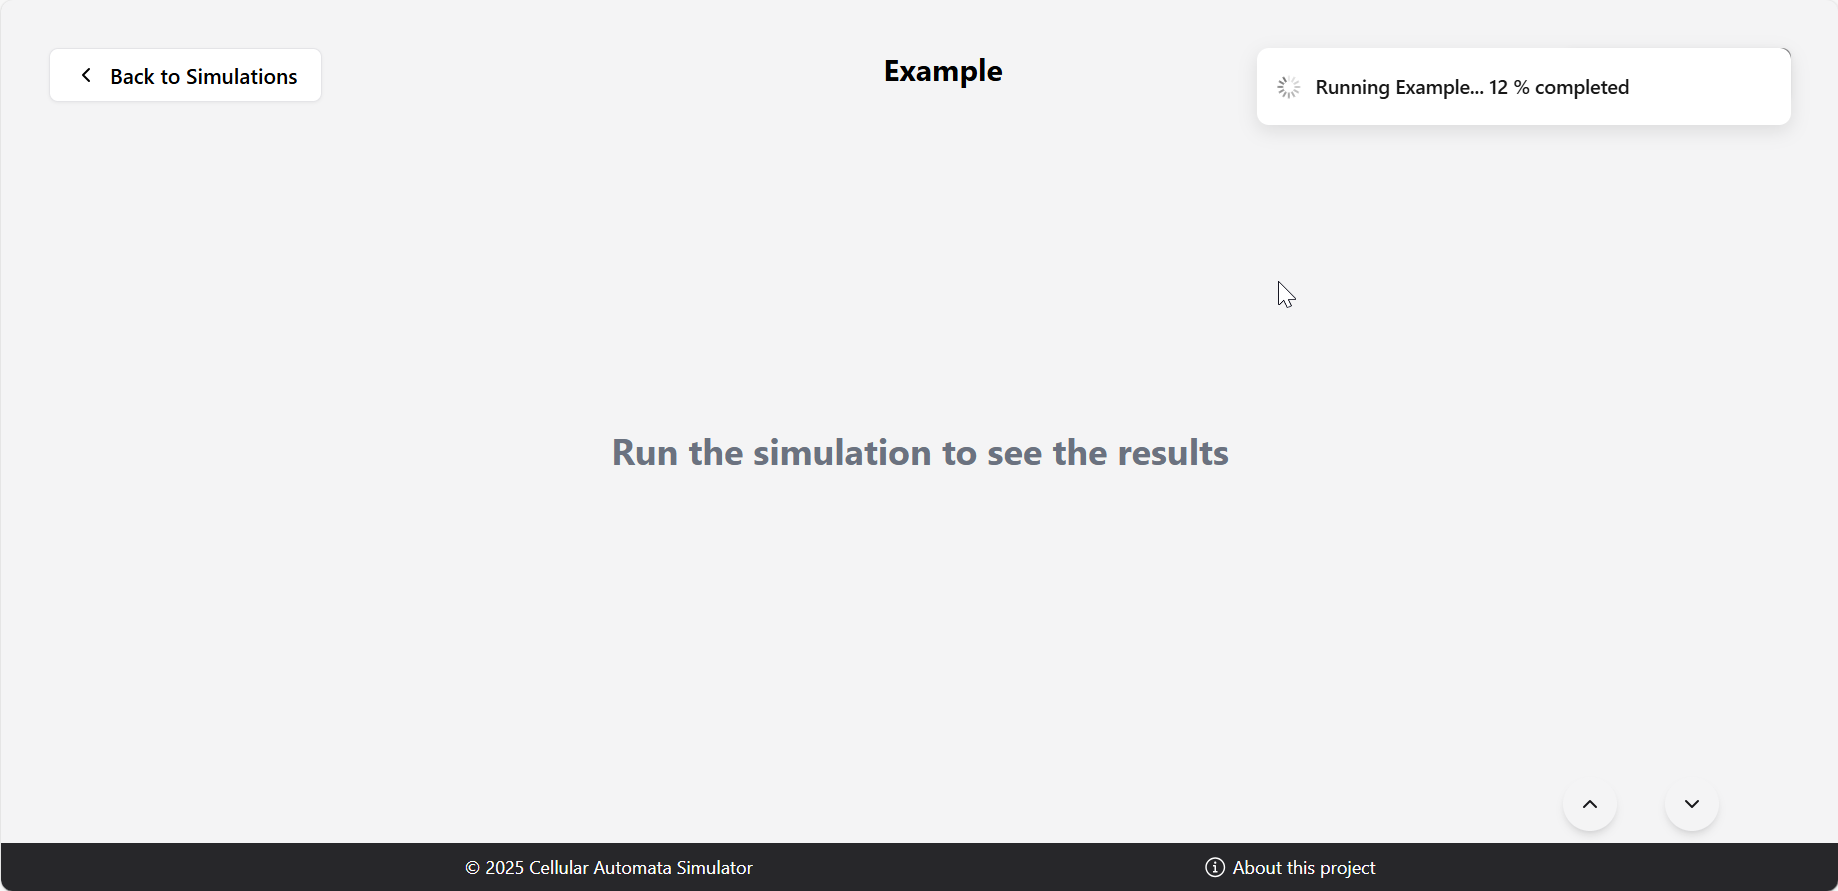
\includegraphics[width=1\textwidth]{img/running_simulacao.png}
    \caption{\small Tela de visualização de uma simulação em execução.}
    \label{fig:interface_simulacao_executando}
\end{figure}

Na mesma tela, terminada a execução, o usuário visualiza os resultados da simulação ilustrados na forma de malhas para cada iteração, com uma legenda ao lado para identificação dos componentes distintos por cores. Rolando a malha para baixo é possível conferir as próximas iterações e utilizando o campo de seleção de página no lado direito é possível navegar entre conjuntos de iterações, com cada conjunto contendo até 1000 iterações. A Figura \ref{fig:interface_simulacao_resultados} ilustra a tela de visualização dos resultados de uma simulação já executada.

\begin{figure}[H]
    \centering
    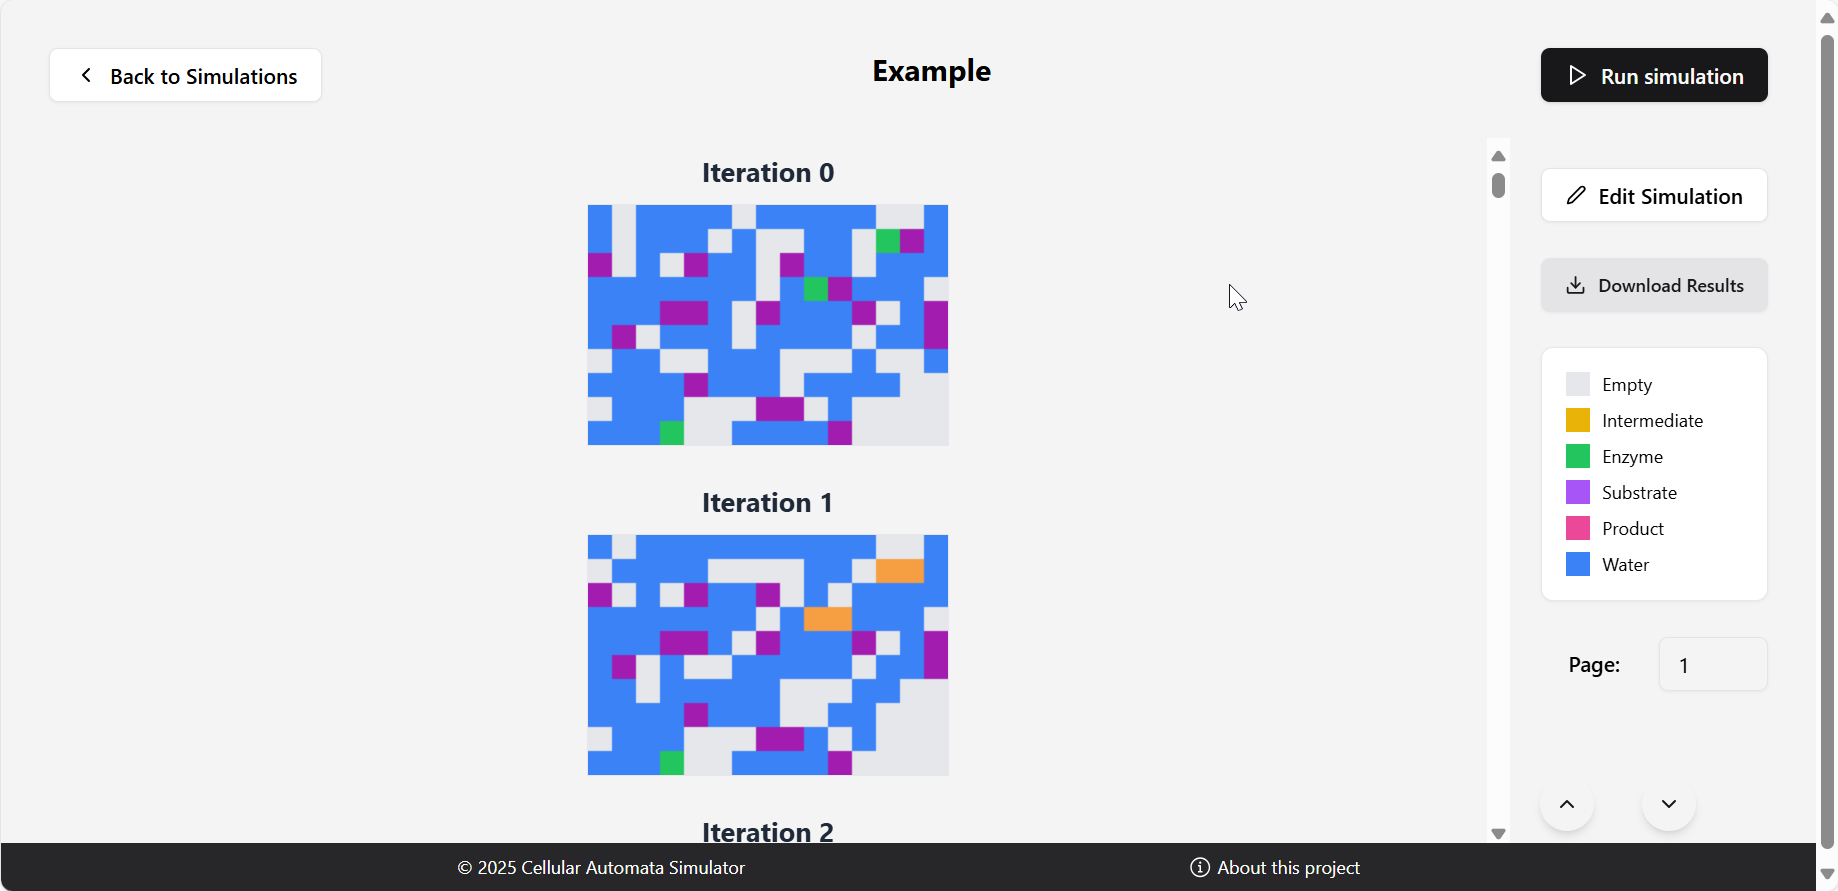
\includegraphics[width=1\textwidth]{img/result_simulacao.png}
    \caption{\small Tela de visualização dos resultados de uma simulação já executada.}
    \label{fig:interface_simulacao_resultados}
\end{figure}

A separação da visualização das iterações em páginas é uma estratégia para melhorar a performance da interface, visto que a quantidade de dados a ser renderizada na tela pode ser muito grande, o que tornaria a renderização lenta e pesada se todas as iterações fossem carregadas de uma vez. Assim, o usuário pode navegar pelas iterações conforme necessário, sem comprometer a fluidez da interface.

O botão \textbf{Download Results} permite que o usuário baixe os resultados de frações de todos os componentes da simulação em um arquivo CSV, que pode ser aberto em qualquer editor de planilhas, como o Microsoft Excel ou o Google Sheets, ou até mesmo em qualquer editor de texto, como o Bloco de Notas do sistema operacional. Isso facilita a análise dos dados e a criação de gráficos e tabelas para visualização dos resultados. A
Figura \ref{fig:interface_simulacao_download} ilustra um arquivo CSV de exemplo baixado pelo software, aberto no Microsoft Excel.

\begin{figure}[H]
    \centering
    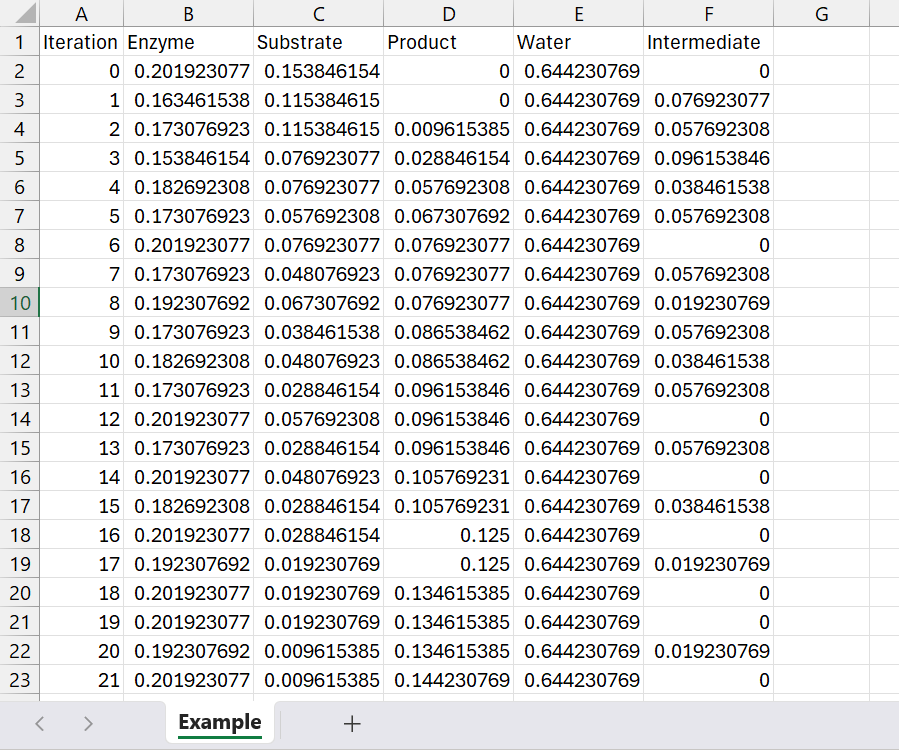
\includegraphics[width=0.8\textwidth]{img/example_csv.png}
    \caption{\small Exemplo de arquivo CSV baixado pelo software, aberto no Microsoft Excel.}
    \label{fig:interface_simulacao_download}
\end{figure}

As colunas são formadas pelo número da iteração (iteração 0 é o estado inicial) e cada componente é uma coluna, com a respectiva fração relativa relacionada à quantidade total de células ocupadas.

\subsection{Ambiente Computacional}

O ambiente computacional utilizado para as simulações foi um computador com as seguintes especificações:
\begin{itemize}
    \item \textbf{Processador}: Intel Core i7-1355U, 10 núcleos, 12 threads, com frequência base de 1.70 GHz e turbo boost de até 5.0 GHz.
    \item \textbf{Memória RAM}: 32 GB DDR4 a 3200 MHz.
    \item \textbf{Sistema Operacional}: Windows 11 24H2 e Ubuntu 24.04 LTS (Linux).
    \item \textbf{Banco de Dados}: PostgreSQL 16.
    \item \textbf{Python}: Versão 3.12 com as bibliotecas \textit{NumPy}, \textit{FastAPI} e \textit{SQLAlchemy} instaladas.
\end{itemize}

O código foi otimizado para garantir um desempenho eficiente, utilizando estruturas de dados adequadas e evitando operações desnecessárias dentro da sua proposta. O tempo de execução das simulações varia conforme o tamanho da grade e o número de iterações. Outro fator que impacta no tempo de execução é a utilização do computador em outras tarefas enquanto a simulação está em andamento. Durante as execuções para a geração dos resultados para este trabalho, o software foi capaz de processar 10000 iterações em grades de $100 \times 100$ células em torno de 45 minutos, com nenhuma ou baixa utilização do computador em tarefas alheias.

Como ocorre em muitos softwares desenvolvidos para resolver problemas complexos por meio de cálculos iterativos extensos, o principal gargalo de desempenho deste modelo está relacionado ao uso da CPU, uma vez que a execução ocorre de forma sequencial, sem paralelização. O consumo de memória, por outro lado, tende a não aumentar significativamente ao longo do tempo, pois, embora o programa armazene temporariamente as configurações das grades de cada iteração, a maior parte dessas informações está estruturada em arrays de números inteiros de 16 bits (números que representam os componentes na malha). Esses arrays ocupam consideravelmente menos espaço em memória quando comparados a estruturas baseadas em strings (caracteres de texto).

De fato, sempre que uma simulação longa está sendo processada, o uso de CPU pelo processo do Python no sistema operacional aumenta e muitas vezes chega a cerca de 95\% de utilização de um núcleo, enquanto o uso de memória RAM permanece abaixo de 10\%. Isso indica que o modelo é eficiente em termos de uso de memória, mas pode ser otimizado para melhorar o desempenho em computação massiva. Perdas de performance do computador ou do sistema operacional em si são quase imperceptíveis, visto que o Python por padrão ocupa somente um núcleo da CPU. No entanto, o modelo implementado possui boa margem de melhoria na eficiência computacional.

O tempo de execução pode ser reduzido significativamente com a implementação de técnicas de paralelização, como o uso de \textit{multiprocessing}, que permite a execução simultânea de múltiplas iterações ou células, aproveitando melhor os recursos do processador.

\chapter{RESULTADOS}

Foram executadas diversas simulações utilizando o modelo de autômato celular implementado, com o objetivo de analisar o comportamento do sistema sob diferentes condições e parâmetros. As simulações foram configuradas para explorar a dinâmica de reações enzimáticas, considerando a movimentação dos componentes químicos, as reações entre eles e a rotação dos componentes rotacionáveis. Após executar cada simulação, os resultados referentes às frações relativas de componentes ao longo de todas as iterações foram baixados pela função do próprio software como arquivo CSV e, então, analisados.

A análise dos resultados foi realizada com o auxílio das bibliotecas \textit{Pandas} (\citetitle{pandas}), \textit{Matplotlib} (\citetitle{matplotlib}) e \textit{Scikit-learn} do Python. \textit{Pandas} é uma biblioteca bastante conhecida no ambiente de tratamento de dados, pois permite a leitura e manipulação de dados de forma eficiente e intuitiva. \textit{Matplotlib} é uma biblioteca de visualização de dados que permite a criação de gráficos e plots de forma simples, permitindo criar gráficos dos mais variados tipos e estilos, além de integrar muito bem com \textit{Pandas}. \textit{Scikit-learn} é uma biblioteca bastante útil para análise estatística e aprendizado de máquina, que oferece diversas ferramentas para análise de dados, incluindo regressão, classificação e clustering. Essas bibliotecas foram utilizadas para processar os dados de frações relativas das simulações, gerar gráficos e realizar análises estatísticas dos resultados.

\section{Cinética Clássica de Michaelis-Menten}

A intenção dessa análise é reproduzir o comportamento clássico da cinética enzimática de Michaelis-Menten, onde a enzima se liga ao substrato em uma reação reversível para formar um complexo enzima-substrato, que posteriormente se converte em produto em uma reação irreversível. Para isso, foram definidos os parâmetros básicos e reacionais demonstrados na Tabela \ref{tab:params_michaelis_menten} e ilustrados nas Figuras \ref{fig:michaelis_menten} e \ref{fig:michaelis_menten_reaction}.

\begin{table}[H]
    \centering
    \caption{Parâmetros da Simulação de Cinética Clássica de Michaelis-Menten}
    \vspace{0.2cm}
    \begin{tabularx}{\textwidth}{X m{5cm}}
        \hline
        \textbf{Parâmetro}                     & \textbf{Valor}   \\
        \hline
        Número de iterações                    & 15000            \\
        Dimensões da malha                     & $100 \times 100$ \\
        Fração de Células de Enzima            & 3\%              \\
        Fração de Células de Substrato         & 15\%             \\
        Fração de Células de Produto           & 0\%              \\
        Fração de Células de Água              & 82\%             \\
        $P_R$ da reação $E + S \rightarrow ES$ & 1                \\
        $P_R$ da reação $ES \rightarrow E + P$ & 0{,}001          \\
        $P_R$ da reação $ES \rightarrow E + S$ & 0{,}0001         \\
        $P_R$ da reação $E + P \rightarrow ES$ & 0                \\
        \hline
    \end{tabularx}
    \vspace{0.2cm}
    \makebox[\linewidth][l]{\small Fonte: Autoria própria}
    \label{tab:params_michaelis_menten}
\end{table}

\begin{figure}[H]
    \centering
    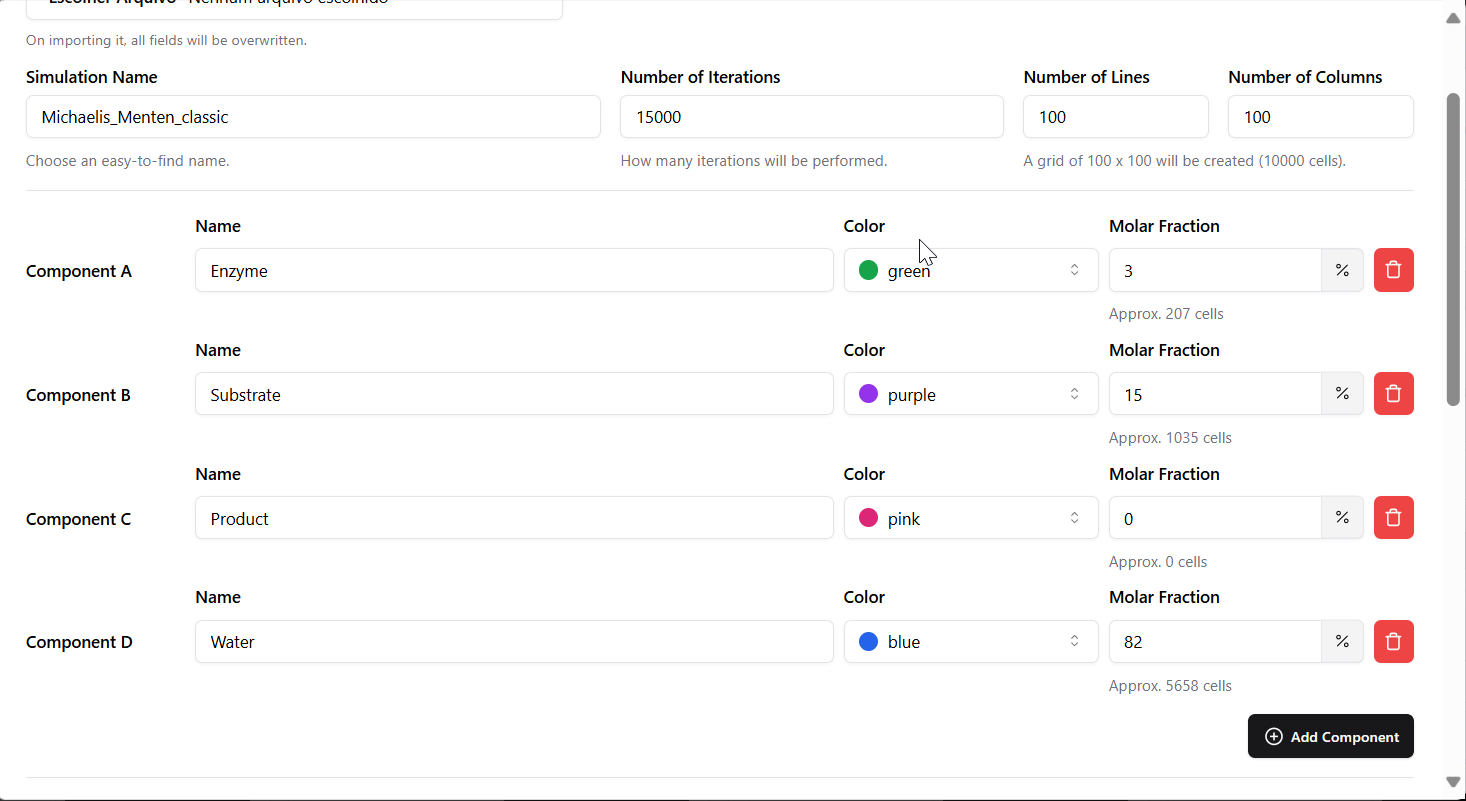
\includegraphics[width=1\textwidth]{img/basic_MM.png}
    \caption{\small Configuração básica e frações relativas de componentes da simulação de cinética clássica de Michaelis-Menten.}
    \label{fig:michaelis_menten}
\end{figure}

\begin{figure}[H]
    \centering
    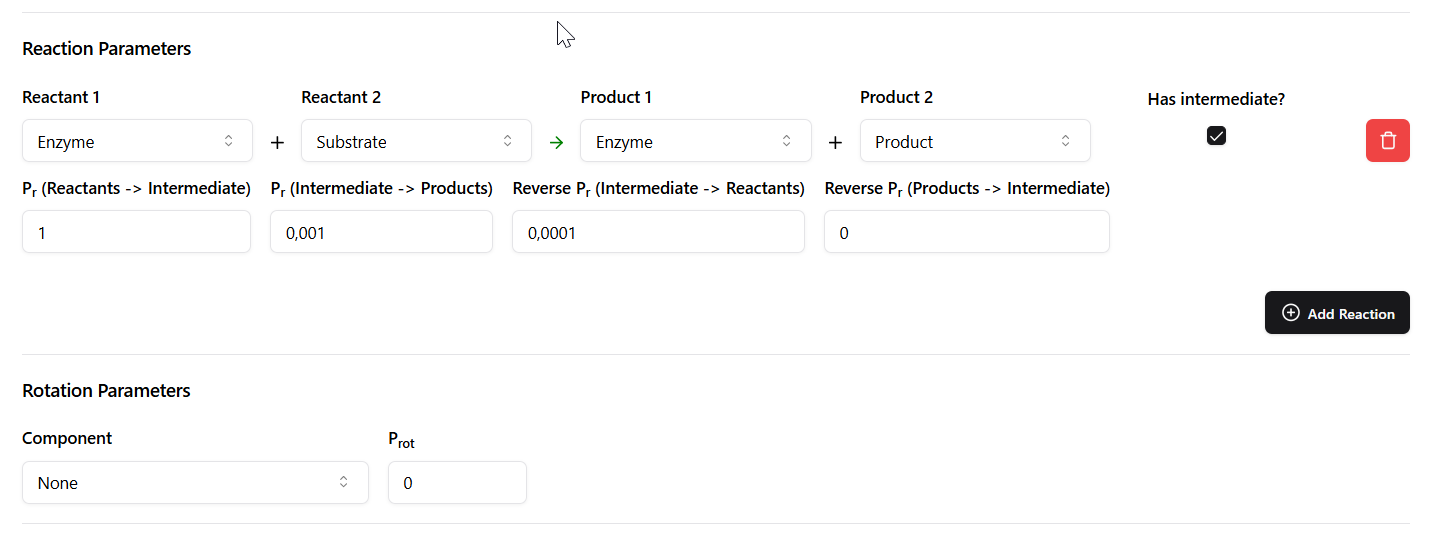
\includegraphics[width=1\textwidth]{img/reaction_MM.png}
    \caption{\small Reações de formação do complexo enzima-substrato e conversão em produto na simulação de cinética clássica de Michaelis-Menten.}
    \label{fig:michaelis_menten_reaction}
\end{figure}

A escolha de 15000 iterações foi feita para garantir que, próximo do final da execução da simulação, o sistema já tenha pouquíssima ou nenhuma reação, com concentração de substrato próxima de zero, o que indica que a enzima já não está mais reagindo com o substrato. Uma malha de $100 \times 100$ células (10000 células no total) é suficiente para observar graficamente o comportamento do sistema e ao mesmo tempo simular a presença de uma quantidade considerável de espécies químicas sem comprometer muito o tempo de execução total da simulação. As frações relativas foram escolhidas para simular um experimento real, onde a enzima está presente em quantidade bem abaixo do substrato em um meio aquoso.

Em relação aos parâmetros de reação, definiu-se que sempre que substrato e enzima se encontrarem, eles irão formar o complexo enzima-substrato, entrando com o $P_R$ dessa etapa igual a 1. A reação inversa, onde o complexo se decompõe em enzima e substrato, ocorre com probabilidade $P_R = 0{,}0001$, o que simula uma reação reversível onde a formação do complexo é favorecida. A conversão do complexo em produto ocorre com probabilidade $P_R = 0{,}001$, o que simula a etapa lenta da reação geral e favorece a formação do produto. O mecanismo clássico de Michaelis-Menten propõe que a reação entre enzima e produto para formação do complexo não ocorre, portanto, o $P_R$ dessa etapa é 0.

Definiu-se os parâmetros de movimentação dos componentes da forma exposta na Tabela \ref{tab:params_movimento} e na Figura \ref{fig:michaelis_menten_movement}:

\begin{table}[H]
    \centering
    \caption{Parâmetros de Movimento para Simulação de Cinética Clássica de Michaelis-Menten}
    \vspace{0.2cm}
    \begin{tabularx}{\textwidth}{X m{5cm}}
        \hline
        \textbf{Parâmetro} & \textbf{Valor} \\
        \hline
        $P_M$ (E)          & 0{,}98         \\
        $P_M$ (S)          & 0{,}99         \\
        $P_M$ (P)          & 0{,}99         \\
        $P_M$ (W)          & 1              \\
        $J$ (E$|$E)        & 0              \\
        $J$ (E$|$S)        & 1{,}7          \\
        $J$ (S$|$S)        & 0              \\
        $J$ (E$|$P)        & 1{,}4          \\
        $J$ (S$|$P)        & 1{,}7          \\
        $J$ (P$|$P)        & 0              \\
        $J$ (E$|$W)        & 1{,}7          \\
        $J$ (S$|$W)        & 1{,}7          \\
        $J$ (P$|$W)        & 1{,}7          \\
        $J$ (W$|$W)        & 2{,}5          \\
        \hline
    \end{tabularx}
    \vspace{0.2cm}
    \makebox[\linewidth][l]{\small Fonte: Autoria própria}
    \label{tab:params_movimento}
\end{table}

\begin{figure}[H]
    \centering
    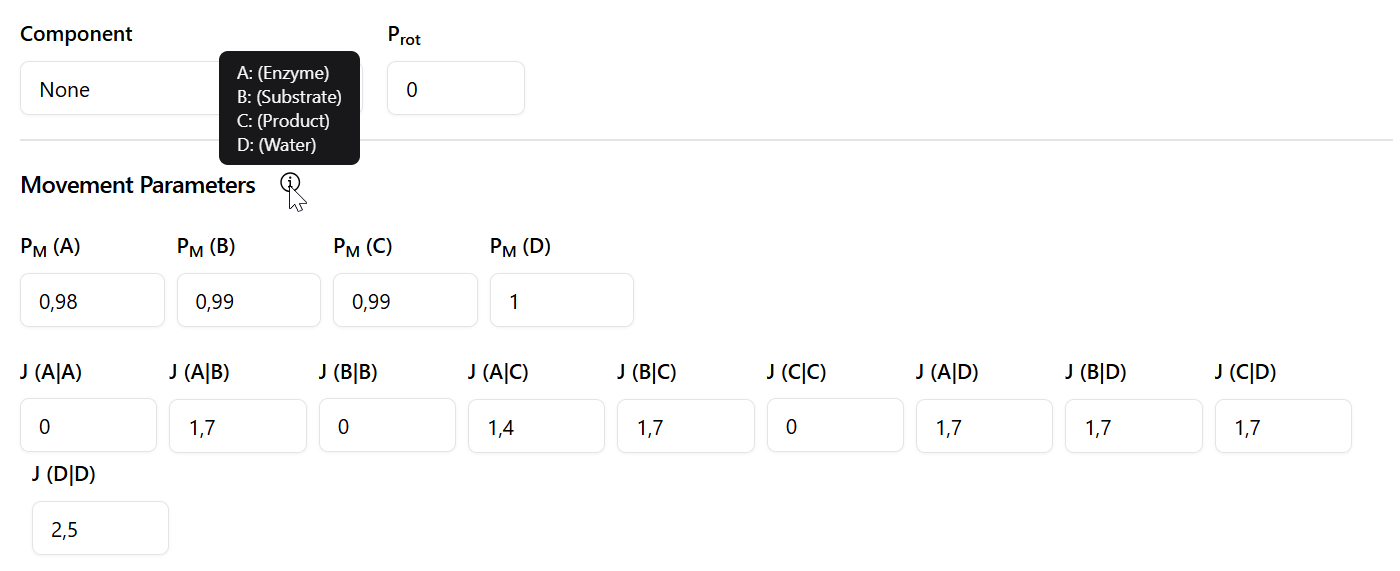
\includegraphics[width=1\textwidth]{img/movement_MM_S0.png}
    \caption{\small Parâmetros de movimentação dos componentes da simulação de cinética clássica de Michaelis-Menten.}
    \label{fig:michaelis_menten_movement}
\end{figure}

Esses valores de movimentação e interação foram escolhidos para simular um sistema bastante dinâmico, dados os valores altos de $P_M$ e baixos de $J$, considerando seus limites estabelecidos. Intuitivamente, $P_M$ para a enzima foi escolhido como 0{,}98, sendo o menor valor entre os componentes imaginando sua molécula realisticamente mais pesada entre todos eles. $P_M = 0{,}99$ para o substrato e 0{,}99 para o produto indicam facilidade de movimentação comparativamente intermediária. A água é definida como um componente altamente móvel, com $P_M = 1$, o que simula um meio líquido formado por moléculas bastante leves.

Com o objetivo de simular um sistema em que substrato e enzima são solúveis em água e se aproximar mais das condições para a modelagem pela cinética clássica de Michaelis-Menten, a interação da enzima, do substrato e do produto com a água são definidas como favoráveis à atração, com valores de $J$ de 1{,}7. A interação entre enzima e substrato é definida, também, como atrativa, com $J = 1{,}7$, o que possibilita a formação do complexo enzima-substrato.

Nota-se, pelos mesmos motivos, a boa interação entre enzima e água, além da diferença entre a ligação da enzima com o substrato e dela com o produto. Enzima-substrato foi pensada para ser uma interação maior no sentido de favorecer a formação do complexo, em detrimento da interação com o produto que, segundo a cinética em estudo, não gera reação. O valor de $J (E|P)$ ser um pouco mais baixo também vem da ideia que, após uma reação completa, o produto ``se descola'' da enzima, sugerindo uma interação mais fraca entre eles (com $P_B (E,P)$ um pouco maior, dada a relação inversa entre $J$ e $P_B$).

Os parâmetros $J (S|S)$, $J (P|P)$ e $J (E|E)$ foram definidos como 0, o que significa que não há interação entre células do mesmo tipo, ou seja, enzimas não se atraem entre si, substratos não se atraem entre si e produtos não se atraem entre si. Isso simula um sistema onde as moléculas de cada um desses componentes estão solubilizados em água, sem formação de aglomerados.

Com esses parâmetros, a simulação foi executada e o arquivo CSV resultante foi analisado. O estado inicial da malha, gerado de forma aleatória, é apresentado na Figura \ref{fig:MM_initial}, onde é possível observar a distribuição inicial dos componentes químicos, com enzima (E) em verde, substrato (S) em roxo, produto (P) em rosa, água (W) em azul e intermediário (complexo ES) em amarelo. Células em cinza representam vazios.

\begin{figure}[H]
    \centering
    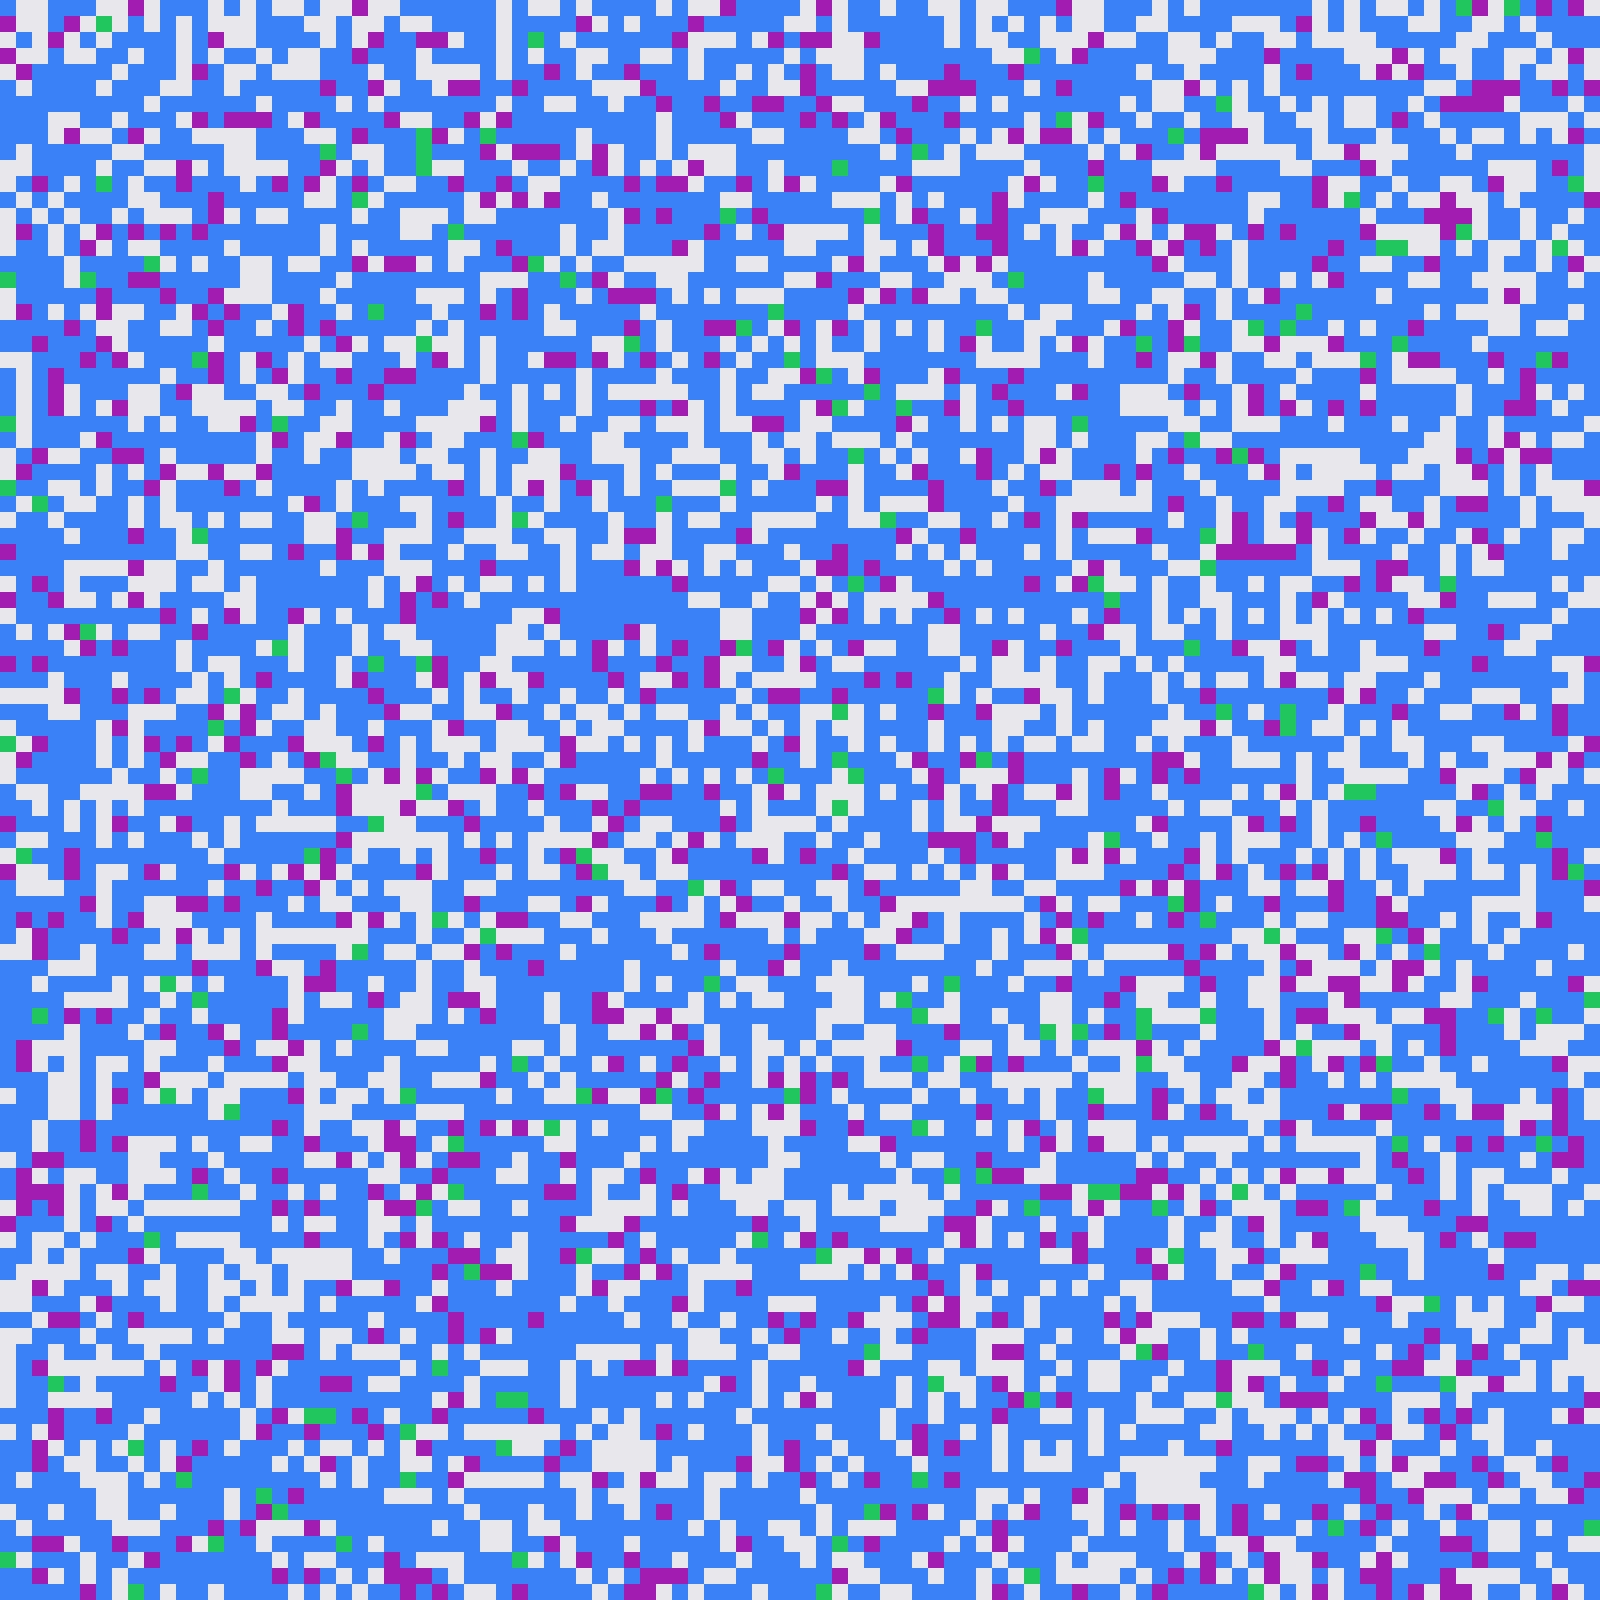
\includegraphics[width=0.7\textwidth]{img/MM_initial_S0.png}
    \hspace{0.05\textwidth}
    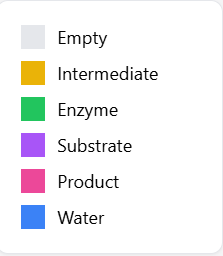
\includegraphics[width=0.2\textwidth]{img/legend.png}
    \caption{\small Estado inicial da malha na simulação de cinética clássica de Michaelis-Menten.}
    \label{fig:MM_initial}
\end{figure}

Nota-se que, nesse momento, não há produto (P) presente, pois a reação ainda não foi iniciada. A enzima (E) e o substrato (S) estão distribuídos aleatoriamente pela malha, enquanto a água (W) ocupa a maior parte das células.

Na Figura \ref{fig:MM_conc}, apresenta-se o gráfico da fração relativa de cada componente ao longo das iterações:

\begin{figure}[H]
    \centering
    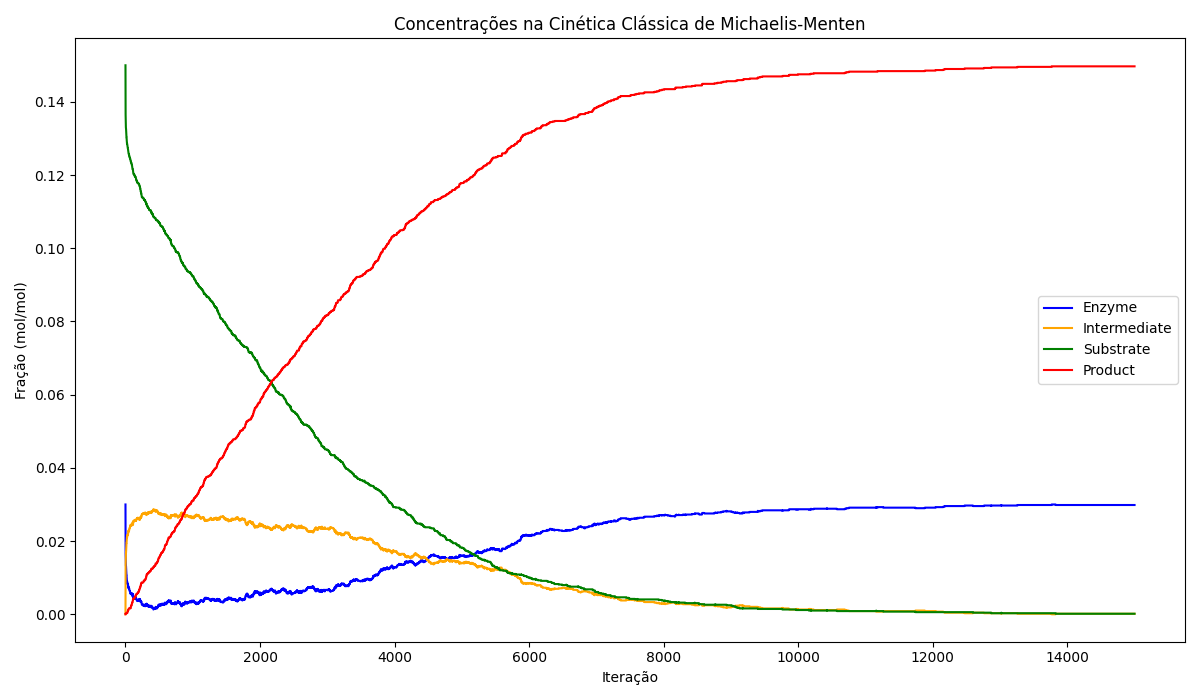
\includegraphics[width=1\textwidth]{img/MM_conc.png}
    \caption{\small Fração relativa (concentração) de cada componente ao longo das iterações na cinética clássica de Michaelis-Menten.}
    \label{fig:MM_conc}
\end{figure}

Importantes tendências são observadas no gráfico da Figura \ref{fig:MM_conc}. Nota-se diminuição abrupta em [S] e [E] com simultâneo aumento em [ES] e [P] durante primeiras iterações, o que indica que a enzima está reagindo com o substrato para formar o complexo enzima-substrato e, posteriormente, o produto. Já por volta de 1000 iterações, observa-se tendência de dinimuição de [ES] e aumento em [E] com aumento de [P], o que indica que o complexo enzima-substrato está se convertendo em produto e disponibilizando novamente a enzima. A Figura \ref{fig:MM_1000it} mostra o estado da malha na iteração 1000, onde se nota a presença significativa do complexo enzima-substrato (ES) e diversas células de produto já formadas.

\begin{figure}[H]
    \centering
    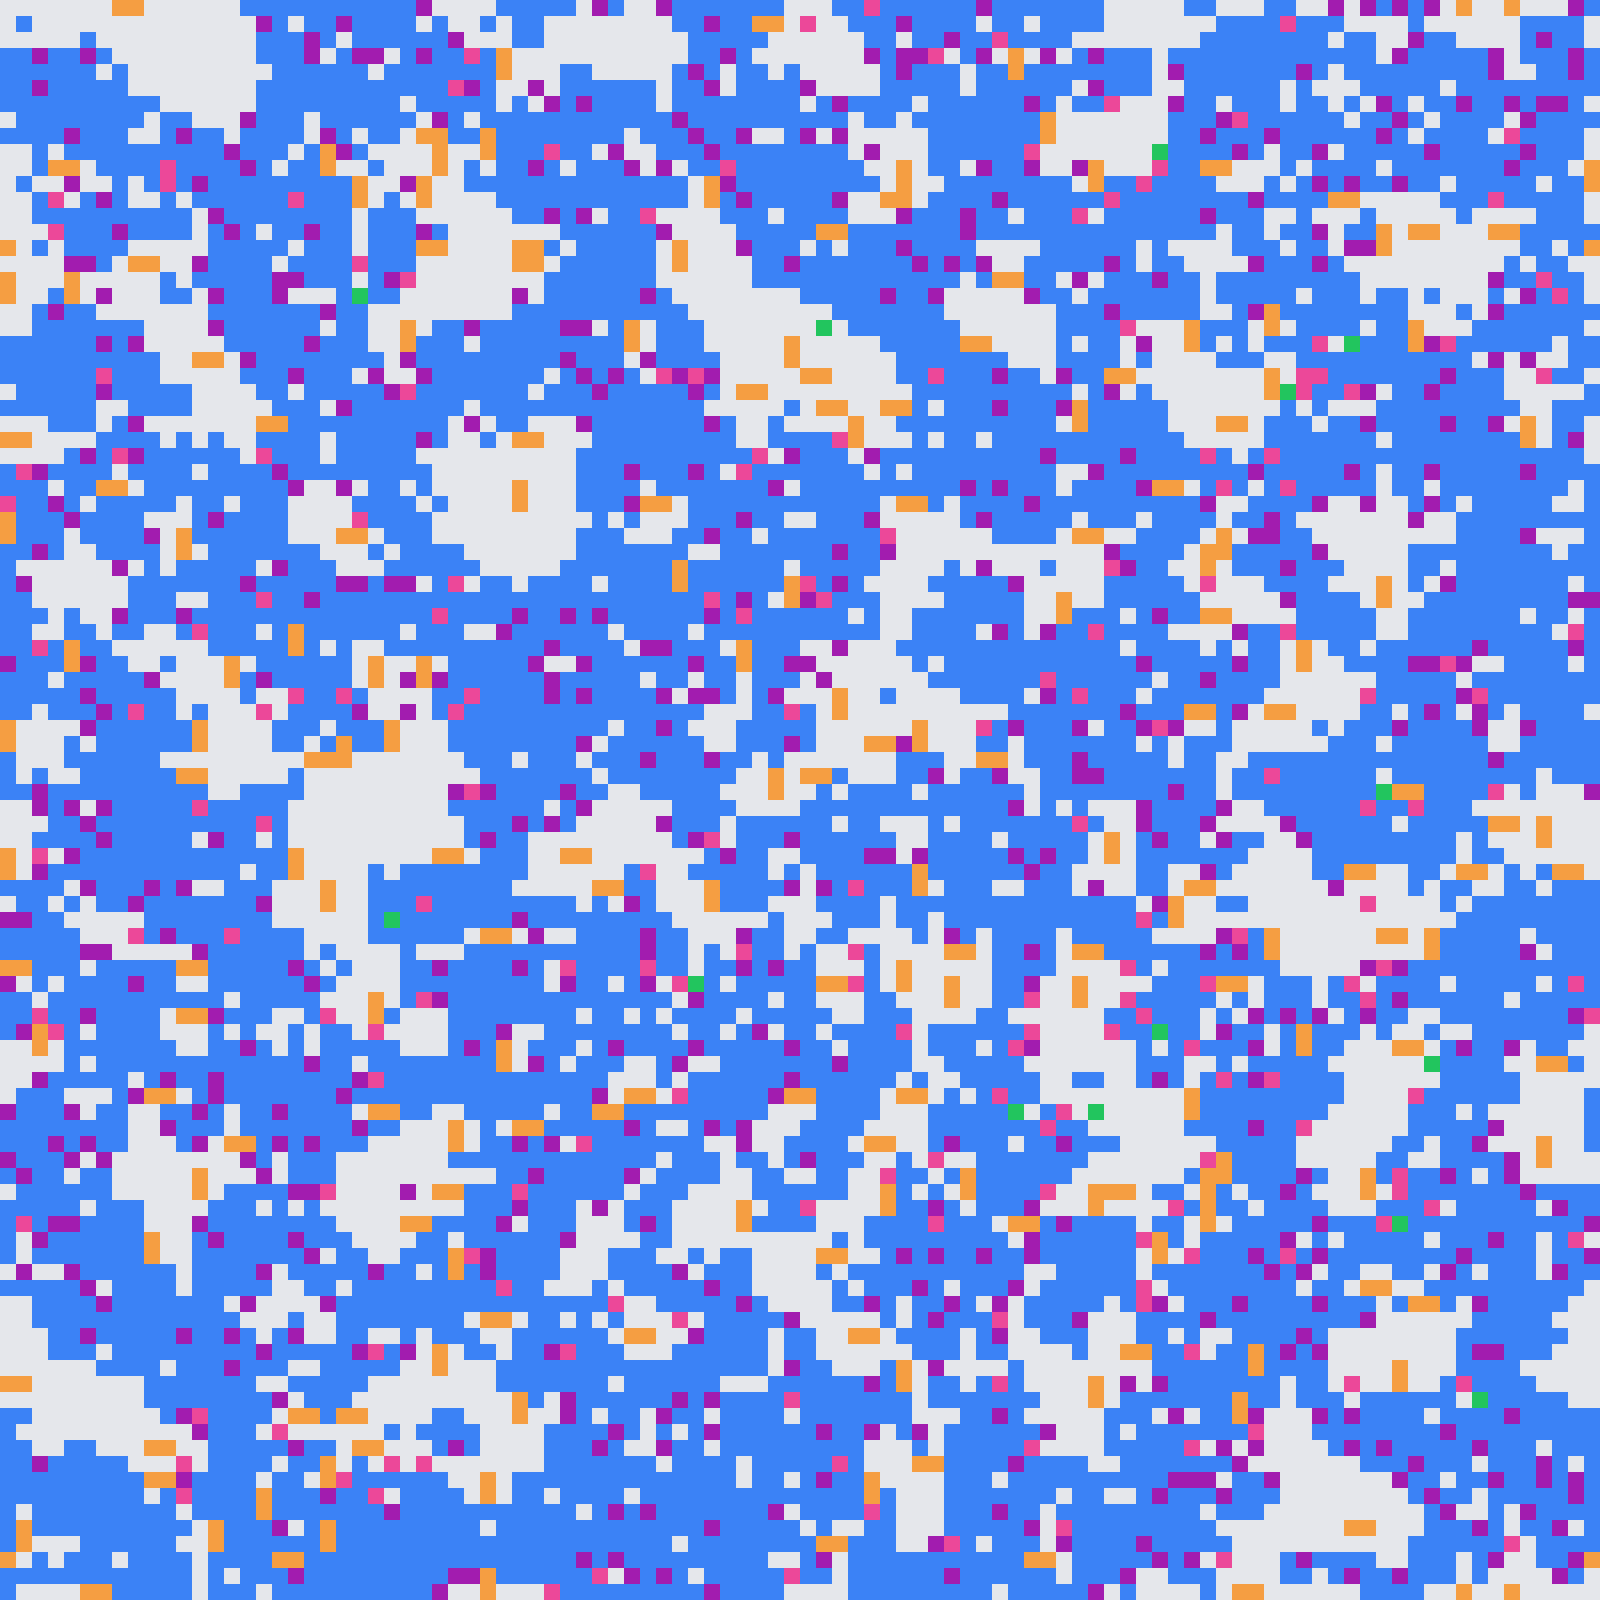
\includegraphics[width=0.7\textwidth]{img/MM_1000it_S0.png}
    \hspace{0.05\textwidth}
    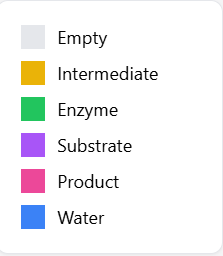
\includegraphics[width=0.2\textwidth]{img/legend.png}
    \caption{\small Estado da malha na iteração 1000 da simulação de cinética clássica de Michaelis-Menten.}
    \label{fig:MM_1000it}
\end{figure}

Por volta de 8000 iterações, [ES] começa a se estabilizar em valores próximos de 0, enquanto [E] vai se tornando assintótica para aproximadamente o valor de sua concentração inicial de 3\% e [P] se estabiliza em torno de 15\%, que é igual à concentração de substrato inicial. Isso indica que, após um certo tempo, a enzima não está mais reagindo com o substrato, pois a concentração de substrato já é praticamente zero. A enzima, portanto, não está mais sendo utilizada e o produto formado permanece no sistema. [ES], por sua vez, se estabiliza em torno de 0, indicando que praticamente todo o complexo enzima-substrato foi convertido em produto.

A Figura \ref{fig:MM_8000it} mostra o estado da malha na iteração 8000, onde se nota a presença significativa de produto (P) e o consumo quase completo de substrato. A boa solubilidade do substrato, da enzima e do produto em água é notória e vem da observação de praticamente todas as células desses componentes cercadas por células de água.

\begin{figure}[H]
    \centering
    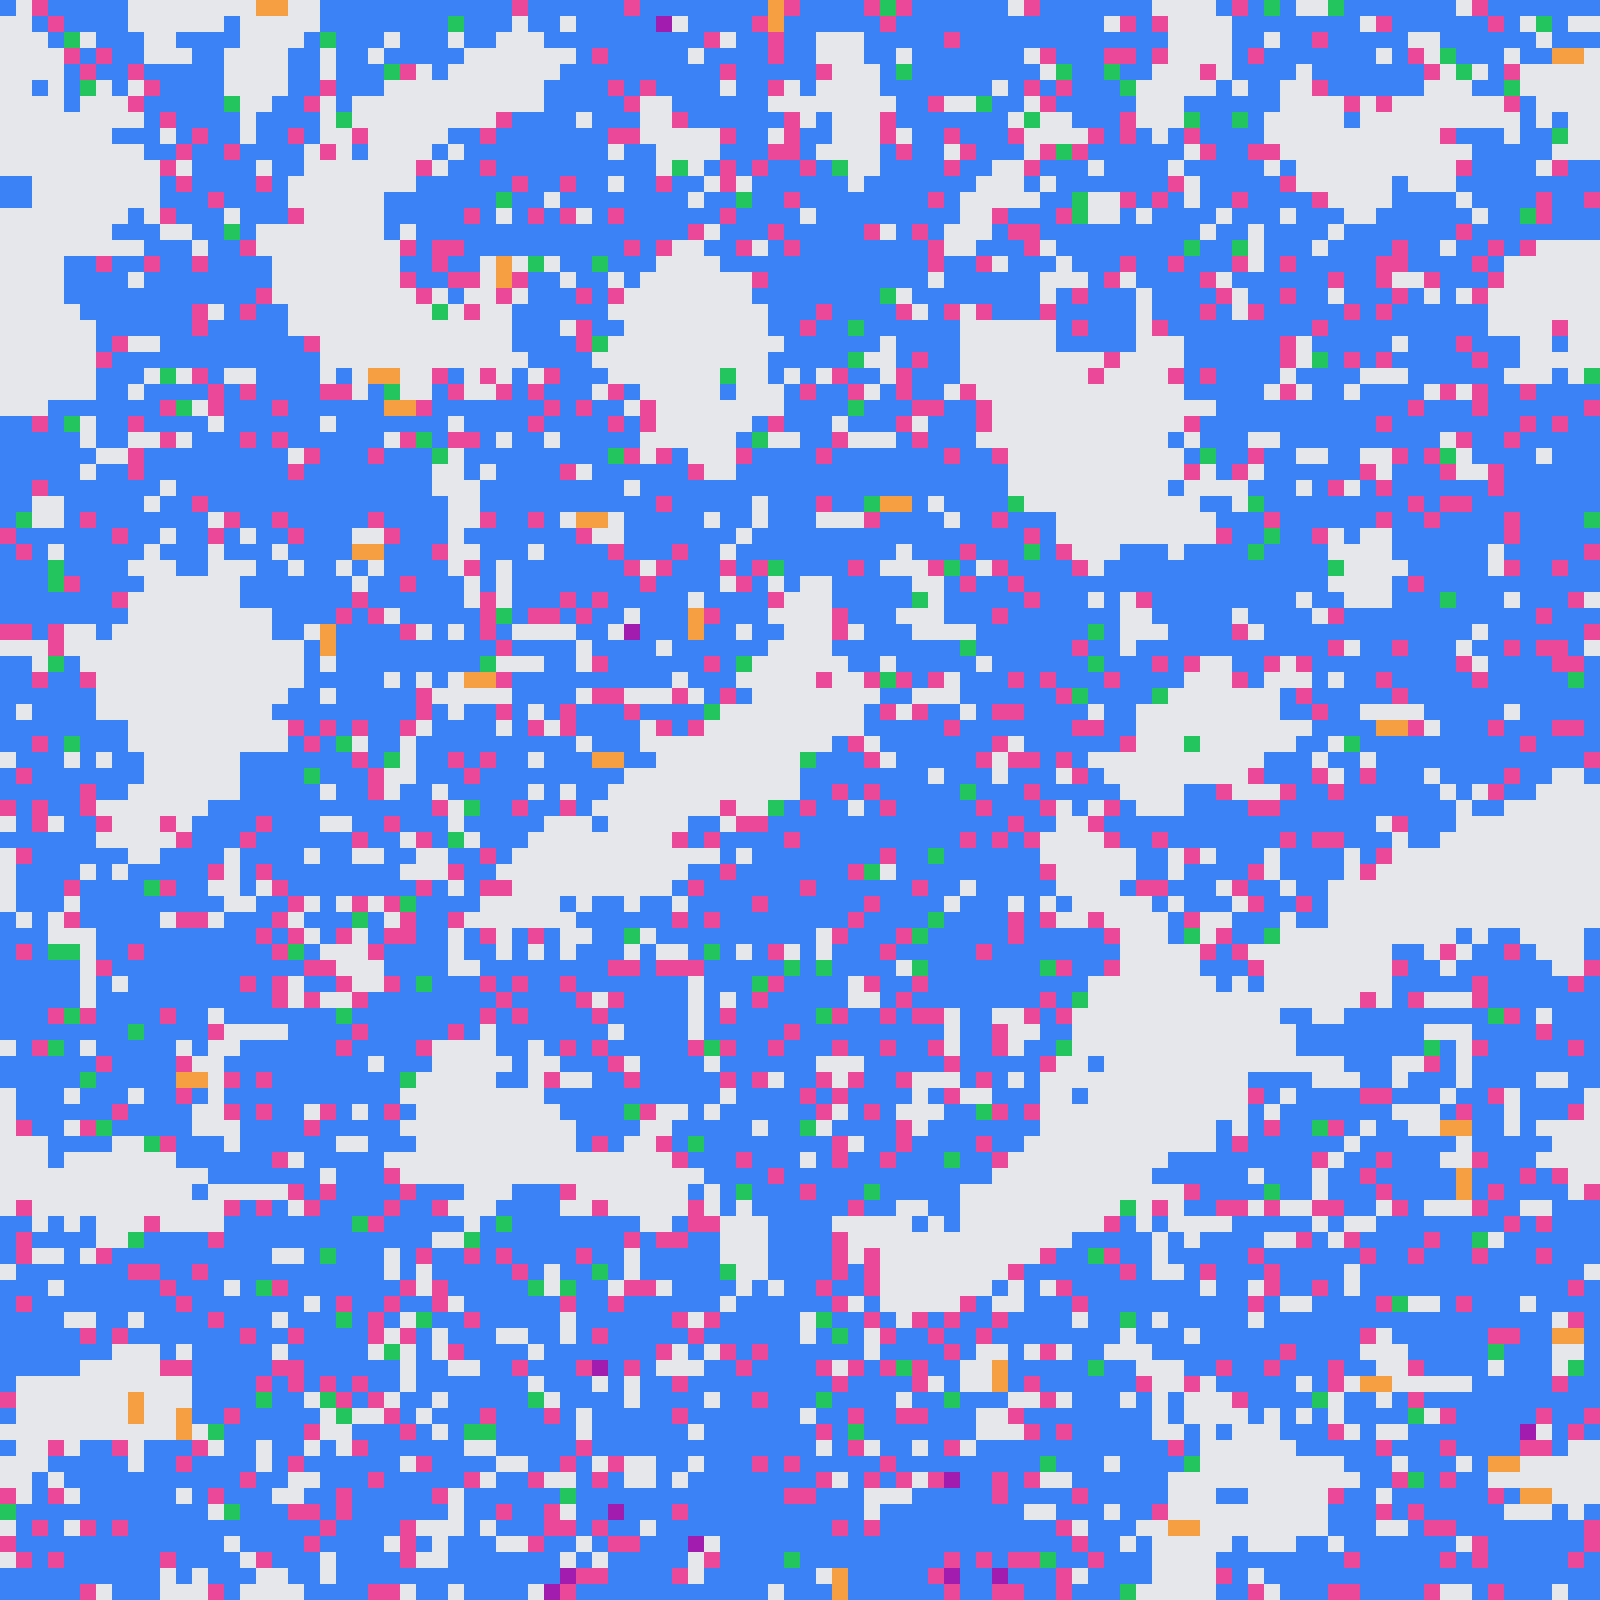
\includegraphics[width=0.7\textwidth]{img/MM_8000it_S0.png}
    \hspace{0.05\textwidth}
    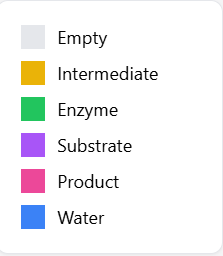
\includegraphics[width=0.2\textwidth]{img/legend.png}
    \caption{\small Estado da malha na iteração 8000 da simulação de cinética clássica de Michaelis-Menten.}
    \label{fig:MM_8000it}
\end{figure}

Esse resultado é consistente com o mecanismo de Michaelis-Menten para cinética enzimática, uma vez que o comportamento das concentrações dos componentes ao longo do tempo segue as tendências esperadas.

Outra análise interessante é a geração da curva de Michaelis-Menten, que relaciona a taxa da reação, que pode ser entendida como a taxa de formação de produto, com a concentração do substrato. Para isso, utilizou-se os dados de concentração do produto ao longo das iterações para fazer uma regressão não-linear, na qual a curva de ajuste é aquela referente à concentração de produto pelo tempo na cinética de Michaelis-Menten, dada por:

\begin{equation}
    \label{eq:produto_MM}
    P(t) = C_1 \left(\frac{1 - e^{C_2 t}}{1 + e^{C_3 t}}\right)
\end{equation}
onde $C_1$, $C_2$ e $C_3$ são constantes a serem ajustadas. A regressão foi realizada utilizando a biblioteca \textit{Scikit-learn} do Python, que oferece ferramentas para ajuste de modelos não-lineares. Após o ajuste, foi possível obter a derivada da curva de formação de produto com o tempo, ou seja, a curva de taxa de formação de produto, que é descrita pela Eq. \ref{eq:taxa_MM} como:

\begin{equation}
    \label{eq:taxa_MM}
    \frac{dP(t)}{dt} = -C_1 C_2 \frac{e^{C_2 t}}{1 + e^{C_3 t}} - C_1 C_3 \frac{(1 - e^{C_2 t}) e^{C_3 t}}{(1 + e^{C_3 t})^2}
\end{equation}
onde $C_1$, $C_2$ e $C_3$ são os mesmos parâmetros ajustados na regressão da curva de formação de produto.

Essa derivada pode ser calculada em Python utilizando a biblioteca \textit{SymPy}, que permite manipulação simbólica de expressões matemáticas. A seguir, apresenta-se o gráfico da concentração de produto e de sua derivada, a taxa da reação, ao longo das iterações:

\begin{figure}[H]
    \centering
    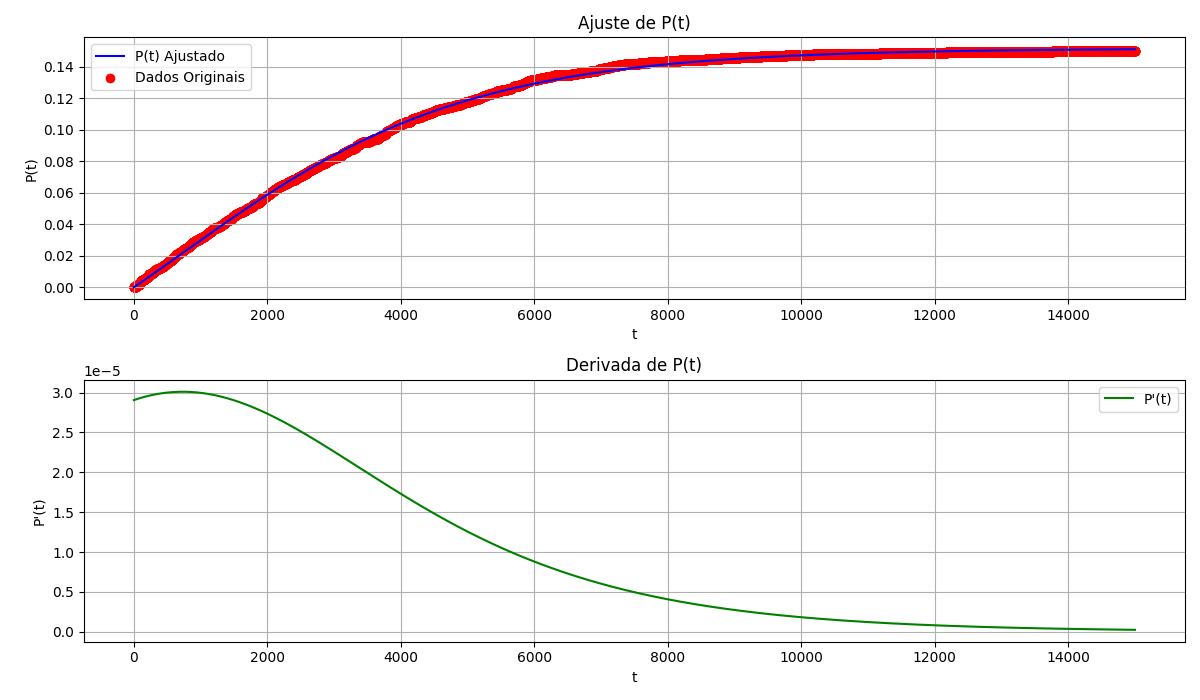
\includegraphics[width=1\textwidth]{img/MM_rate.png}
    \caption{\small Curva de concentração de produto e taxa da reação na cinética clássica de Michaelis-Menten.}
    \label{fig:MM_rate}
\end{figure}

A equação encontrada para a curva de concentração de produto foi:

\begin{equation}
    P(t) = 0{,}1516 \left(\frac{1 - e^{-4 \cdot 10^{-4} t}}{1 + e^{-5 \cdot 10^{-4} t}}\right)
\end{equation}
com $R^2 = 0{,}9991$, indicando um excelente ajuste. A derivada dessa curva, que representa a taxa de formação de produto, é aproximadamente dada por:

\begin{equation}
    P'(t) = 5{,}812 \cdot 10^{-5} \left(\frac{e^{-3{,}834 \cdot 10^{-4} t}}{1 + e^{-4{,}815 \cdot 10^{-4} t}}\right) + 7{,}299 \cdot 10^{-5} \left(\frac{(1 - e^{-3{,}834 \cdot 10^{-4} t}) e^{-4{,}815 \cdot 10^{-4} t}}{(1 + e^{-4{,}815 \cdot 10^{-4} t})^2}\right)
\end{equation}

De posse da taxa de reação, obtem-se o gráfico de Michaelis-Menten, que relaciona a taxa de formação de produto com a concentração de substrato. Na Figura \ref{fig:MM_curve}, apresenta-se o gráfico da curva de Michaelis-Menten:

\begin{figure}[H]
    \centering
    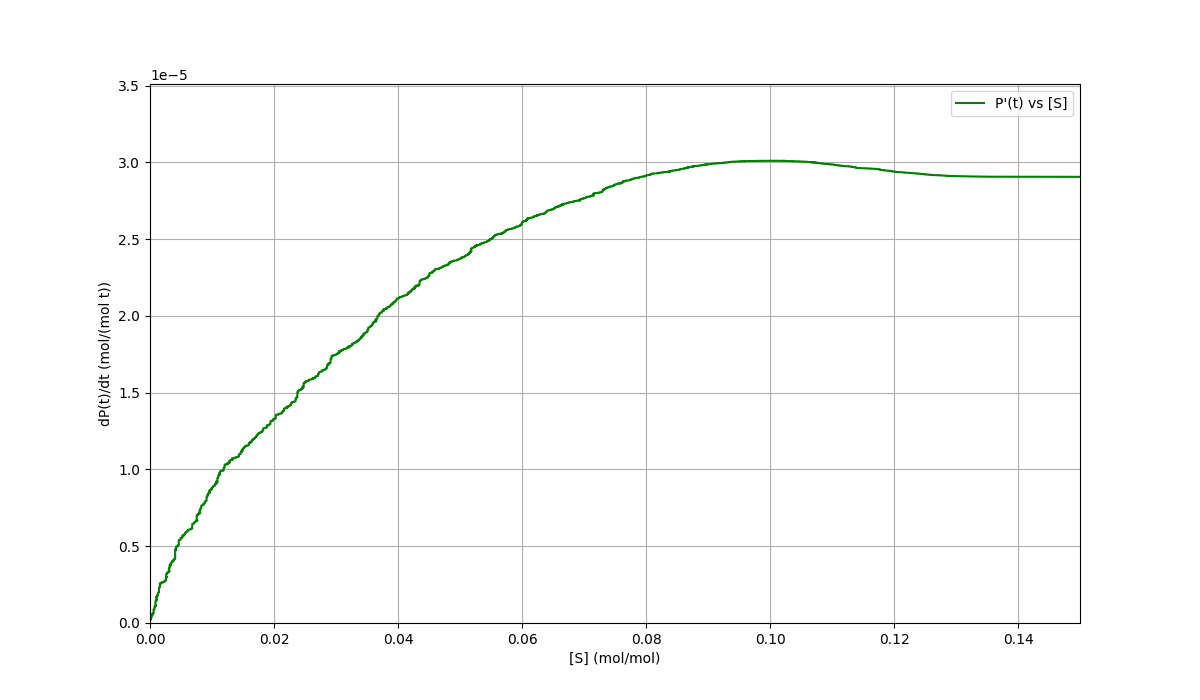
\includegraphics[width=1\textwidth]{img/MM_curve.png}
    \caption{\small Curva de Michaelis-Menten: taxa de formação de produto em função da concentração de substrato.}
    \label{fig:MM_curve}
\end{figure}

A curva de Michaelis-Menten obtida se apresenta de forma muito semelhante ao comportamento típico, onde a taxa de formação de produto aumenta com a concentração de substrato até atingir um platô. O platô revela a $V_{max}$, que é a taxa máxima de formação de produto, com valor muito próximo de $3 \cdot 10^{-5}$. A concentração de substrato na qual a taxa de formação de produto (taxa de reação) atinge metade do valor máximo é conhecida como $K_m$, que é uma medida da afinidade da enzima pelo substrato. No caso desta simulação, $K_m \approx 0{,}0238$.

Em resumo, a tabela \ref{tab:params_MM} apresenta os valores das constantes de Michaelis-Menten obtidas a partir da simulação. A unidade de medida de $V_{max}$ é fração molar por iteração, que pode ser representada como inverso de iteração ($it^{-1}$), enquanto $K_M$ é uma fração molar.

\begin{table}[H]
    \centering
    \caption{Constantes de Michaelis-Menten na Simulação de Cinética Clássica}
    \vspace{0.2cm}
    \begin{tabularx}{\textwidth}{X m{5cm}}
        \hline
        \textbf{Constante} & \textbf{Valor}                    \\
        \hline
        $V_{max}$          & $3{,}01 \cdot 10^{-5} \, it^{-1}$ \\
        $K_M$              & $0{,}0238 \, mol/mol$             \\
        \hline
    \end{tabularx}
    \vspace{0.2cm}
    \makebox[\linewidth][l]{\small Fonte: Autoria própria}
    \label{tab:params_MM}
\end{table}

Foi possível obter, também, o gráfico típico de Lineweaver-Burk, que é uma representação linear da relação entre a taxa de reação e a concentração de substrato, e é mostrado na Figura \ref{fig:MM_lineweaver_burk}. No entanto, essa representação envolve o ajuste linear dos dados, o que ao longo dos experimentos com as simulações não se mostrou tão confiável, embora o coeficiente de correlação tenha sido próximo de 0{,}9, apresentando muita variação de acordo com a faixa de iterações em que a dependência entre a taxa de reação e a concentração de substrato é linear.

\begin{figure}[H]
    \centering
    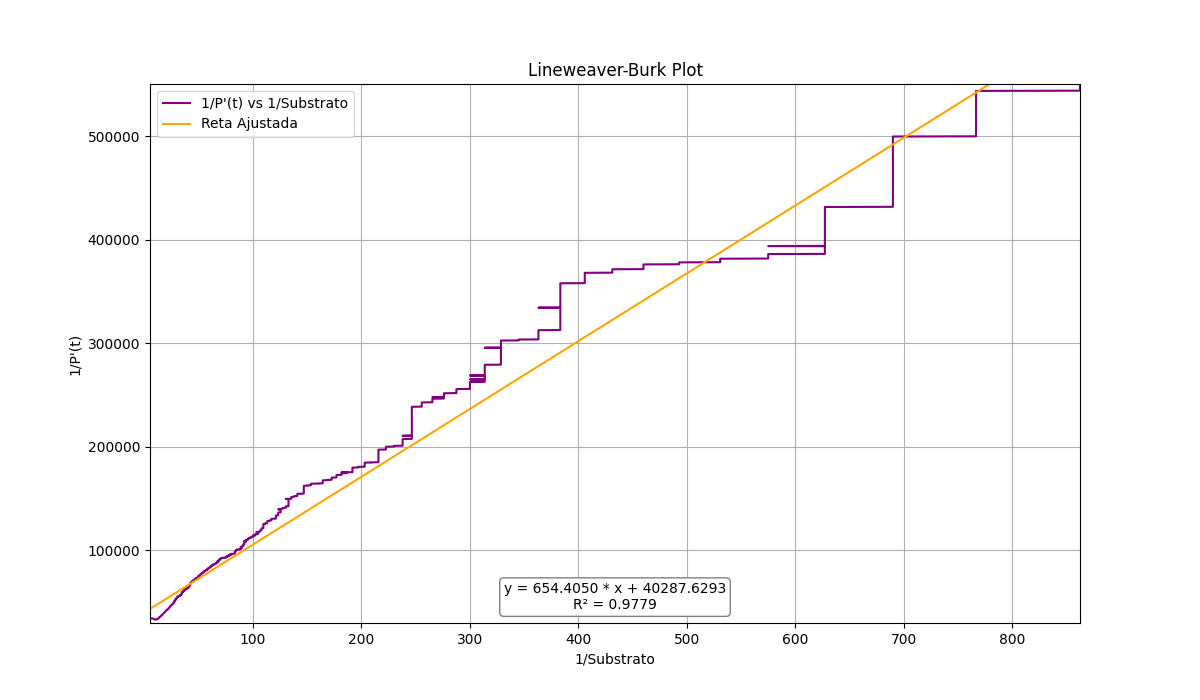
\includegraphics[width=1\textwidth]{img/lineweaver_burk_plot.png}
    \caption{\small Gráfico de Lineweaver-Burk: taxa de reação em função da concentração de substrato.}
    \label{fig:MM_lineweaver_burk}
\end{figure}

Por esse método, o coeficiente linear da equação, $b$, é utilizado para encontrar o valor de $V_{max}$, que é dado por $V_{max} = \frac{1}{b} \approx 2{,}48 \cdot 10^{-5} \, it^{-1}$. O coeficiente angular, $a$, é utilizado para encontrar o valor de $K_M$, que é dado por $K_M = \frac{a}{b} \approx 0{,}0162$. Pela razão descrita anteriormente, esse método será desconsiderado para outras simulações.

A simulação em estudo foi, ainda, executada outras duas vezes, com o objetivo de verificar a reprodutibilidade dos resultados com os mesmos parâmetros. Toda a análise dos dados de frações relativas foi realizada para cada execução, e os resultados de $V_{max}$ e $K_M$ são apresentados na Tabela \ref{tab:params_MM_repeticoes}.

\begin{table}[H]
    \centering
    \caption{Resultados de Repetições da Simulação de Cinética Clássica de Michaelis-Menten}
    \vspace{0.2cm}
    \begin{tabularx}{\textwidth}{X X m{5cm}}
        \hline
        \textbf{Execução} & \textbf{$V_{max} \, (it^{-1})$ }      & \textbf{$K_M$}          \\
        \hline
        1                 & $3{,}010 \cdot 10^{-5}$               & $0{,}0238$              \\
        2                 & $3{,}302 \cdot 10^{-5}$               & $0{,}0205$              \\
        3                 & $2{,}900 \cdot 10^{-5}$               & $0{,}0213$              \\
        \hline
        \textbf{Final}    & $(3{,}071 \pm 0{,}170) \cdot 10^{-5}$ & $0{,}0219 \pm 0{,}0014$ \\
        \hline
    \end{tabularx}
    \vspace{0.2cm}
    \makebox[\linewidth][l]{\small Fonte: Autoria própria}
    \label{tab:params_MM_repeticoes}
\end{table}

\section{Cinética com Substrato Apolar}

A intenção dessa análise é reproduzir o comportamento da cinética de Michaelis-Menten, mas agora considerando a presença de um substrato com característica apolar. Para isso, é razoável imaginar que, para uma comparação justa, tanto os parâmetros básicos do modelo quanto os parâmetros de reação sejam os mesmos da simulação anterior, mas com alterações nos parâmetros de movimentação e interação dos componentes. Apresenta-se a Tabela \ref{tab:params_movimento_apolar} e a Figura \ref{fig:michaelis_menten_movement_apolar} com os parâmetros $P_M$ e $J$ utilizados:

\begin{table}[H]
    \centering
    \caption{Parâmetros de Movimento para Simulação de Cinética com Substrato Apolar}
    \vspace{0.2cm}
    \begin{tabularx}{\textwidth}{X m{5cm}}
        \hline
        \textbf{Parâmetro} & \textbf{Valor} \\
        \hline
        $P_M$ (E)          & 0{,}98         \\
        $P_M$ (S)          & 0{,}99         \\
        $P_M$ (P)          & 0{,}99         \\
        $P_M$ (W)          & 1              \\
        $J$ (E$|$E)        & 0              \\
        $J$ (E$|$S)        & 1{,}1          \\
        $J$ (S$|$S)        & 1{,}7          \\
        $J$ (E$|$P)        & 1{,}4          \\
        $J$ (S$|$P)        & 1{,}7          \\
        $J$ (P$|$P)        & 1{,}7          \\
        $J$ (E$|$W)        & 1{,}7          \\
        $J$ (S$|$W)        & 0{,}5          \\
        $J$ (P$|$W)        & 0{,}5          \\
        $J$ (W$|$W)        & 2{,}5          \\
        \hline
    \end{tabularx}
    \vspace{0.2cm}
    \makebox[\linewidth][l]{\small Fonte: Autoria própria}
    \label{tab:params_movimento_apolar}
\end{table}

\begin{figure}[H]
    \centering
    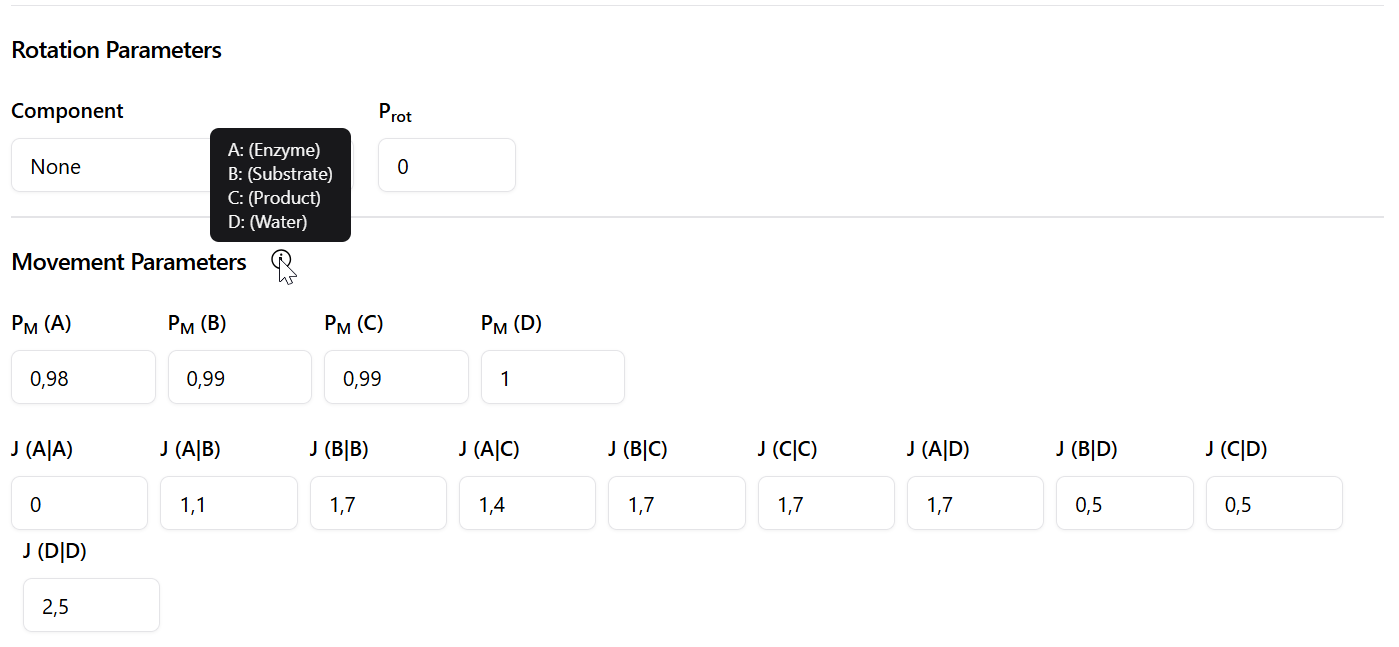
\includegraphics[width=1\textwidth]{img/movement_MM_apolar.png}
    \caption{\small Parâmetros de movimentação dos componentes da simulação de cinética com substrato apolar.}
    \label{fig:michaelis_menten_movement_apolar}
\end{figure}

Comparando com a simulação para Michaelis-Menten clássica, nota-se que foi definido $J (E|S) = 1{,}1$, o que indica uma interação um pouco menos favorável entre enzima e substrato, visto que o substrato agora é apolar. Além disso, $J (S|W) = 0{,}5$ e $J (P|W) = 0{,}5$, o que indica que o substrato e a água se repelem em termos de interação e, dessa forma, é lógico pensar que o produto também será apolar e terá repulsão com a água. Os outros parâmetros são os mesmos da simulação anterior, o que permite uma comparação adequada entre os dois cenários.

Após a execução completa dessa simulação e a análise do arquivo CSV gerado, tem-se os seguintes resultados, começando pelo estado inicial da malha e pelos gráficos de frações relativas de cada componente ao longo das iterações, que são apresentados nas Figuras \ref{fig:MM_apolar_initial} e \ref{fig:MM_apolar_conc}, respectivamente.

\begin{figure}[H]
    \centering
    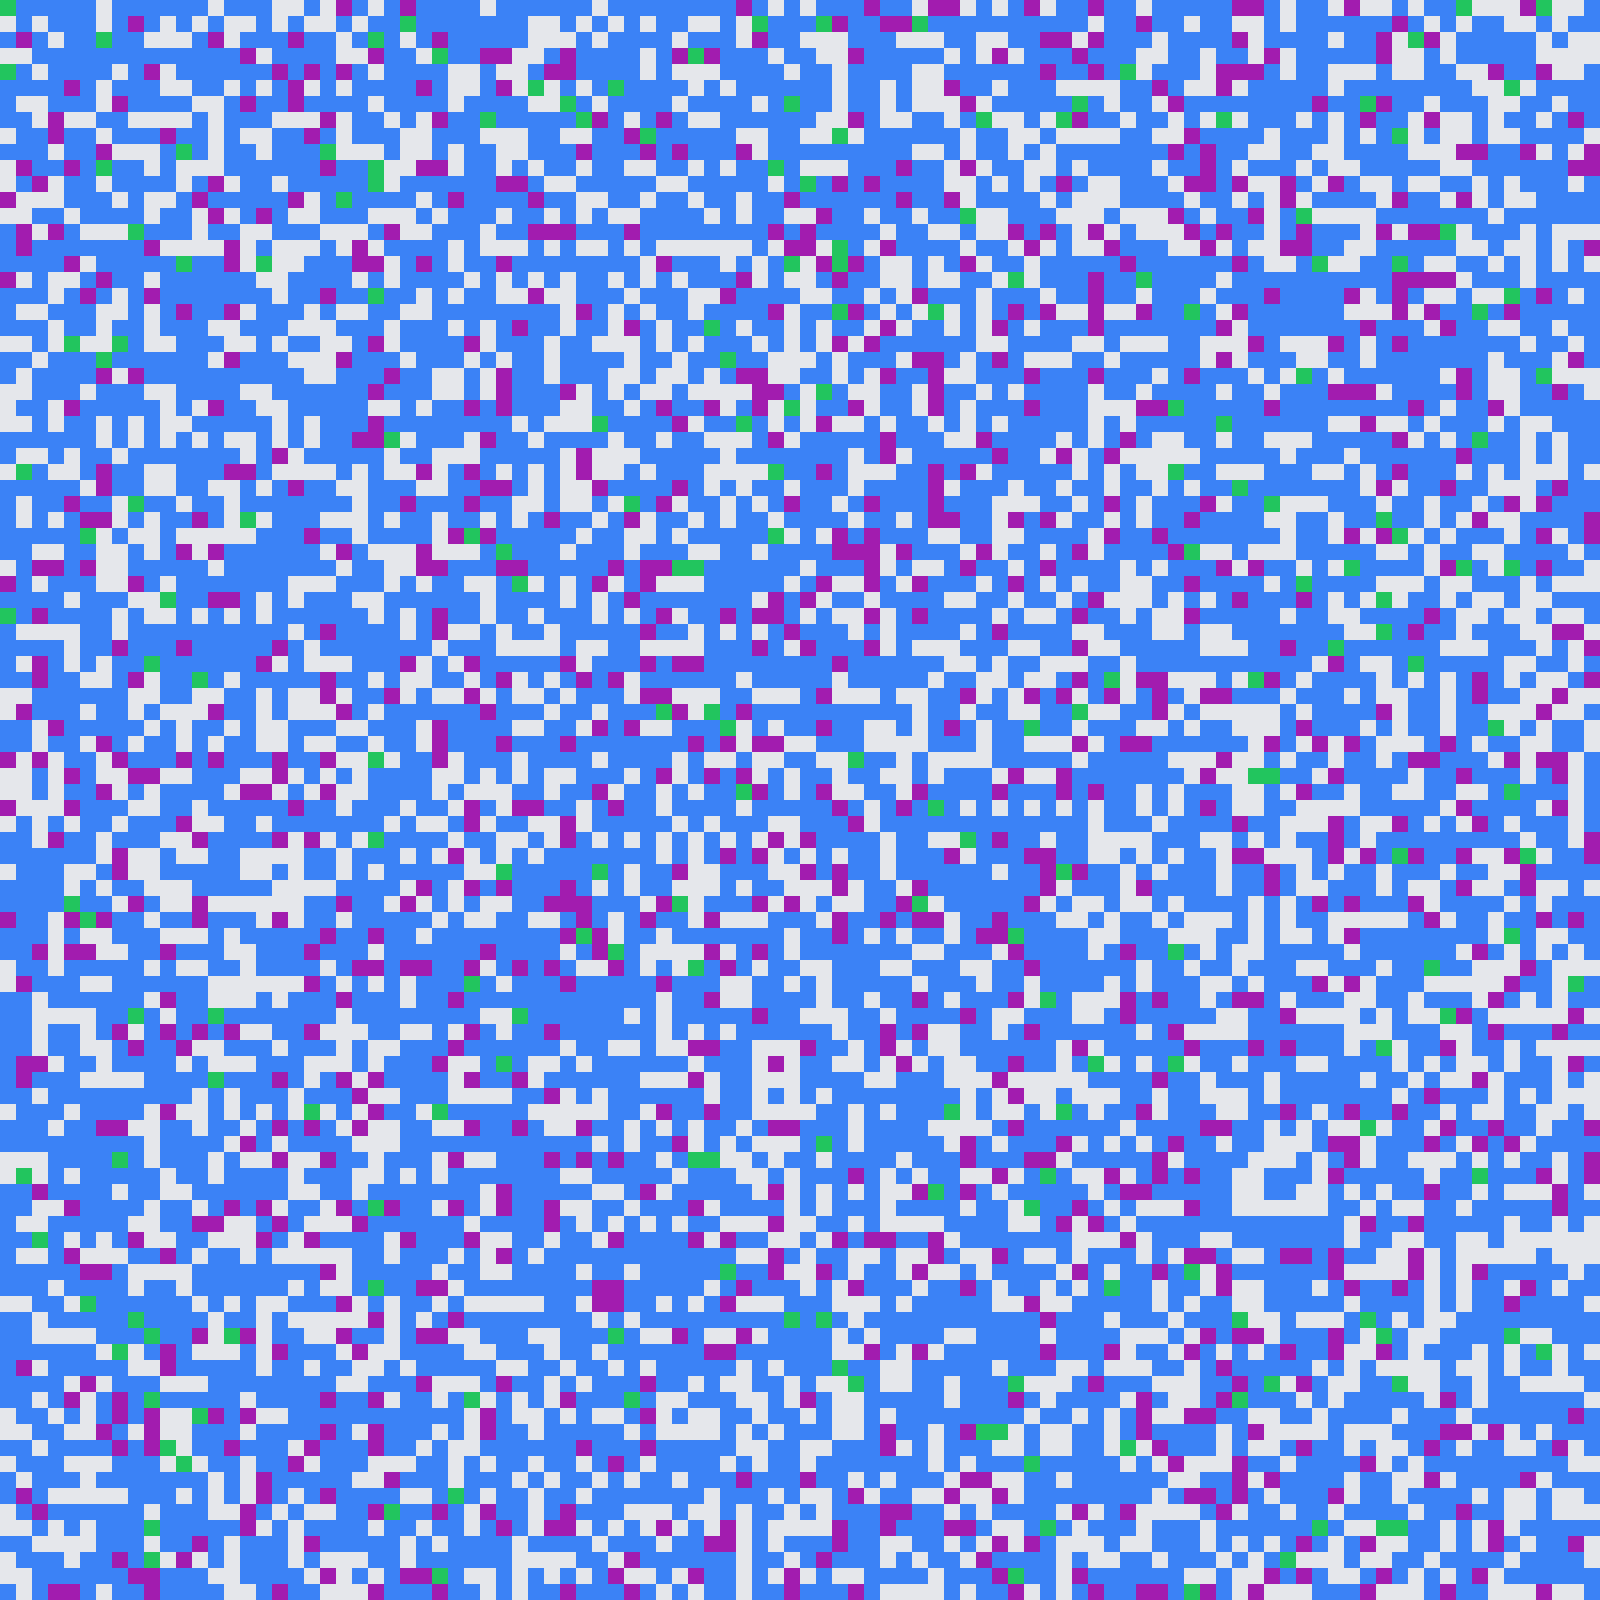
\includegraphics[width=0.7\textwidth]{img/MM_apolar_initial.png}
    \hspace{0.05\textwidth}
    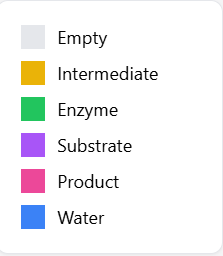
\includegraphics[width=0.2\textwidth]{img/legend.png}
    \caption{\small Estado inicial da malha na simulação de cinética com substrato apolar.}
    \label{fig:MM_apolar_initial}
\end{figure}

\begin{figure}[H]
    \centering
    \includegraphics[width=1\textwidth]{img/MM_apolar_conc.png}
    \caption{\small Fração relativa (concentração) de cada componente ao longo das iterações na cinética com substrato apolar.}
    \label{fig:MM_apolar_conc}
\end{figure}

As curvas são semelhantes às da simulação anterior, com poucas diferenças notáveis. Observa-se que, desta vez, o sistema começa a se estabilizar somente por volta de 10000 iterações, enquanto na simulação anterior a estabilização ocorreu por volta de 8000 iterações. Isso indica que o sistema com substrato apolar é mais lento mesmo mantidos os parâmetros de reação, possivelmente devido à menor interação entre enzima e substrato.

Mais uma diferença a ser notada é a tendência observada de produto e substrato em se aglomerarem em ``bolhas'' ao longo do tempo. Essas bolhas de substrato e produto são visíveis na malha, onde células de substrato e produto se agrupam, formando regiões com alta concentração desses componentes. A água, por sua vez, continua a ocupar a maior parte da malha, mas não interage favoravelmente com o substrato apolar. O comportamento apolar, portanto, é bem reproduzido pelo modelo e pode ser observado na Figura \ref{fig:MM_apolar_3000it}, que mostra o estado da malha na iteração 3000.

\begin{figure}[H]
    \centering
    \includegraphics[width=0.7\textwidth]{img/apolar_3000.png}
    \hspace{0.05\textwidth}
    \includegraphics[width=0.2\textwidth]{img/legend.png}
    \caption{\small Estado da malha na iteração 3000 da simulação de cinética com substrato apolar.}
    \label{fig:MM_apolar_3000it}
\end{figure}

A Figura \ref{fig:MM_apolar_10000it} mostra o estado da malha na iteração 10000, evidenciando a baixa presença de substrato e a formação de aglomerados de produto, devido à sua baixa solubilidade provocada pela escolha dos valores dos parâmetros de movimentação e interação.

\begin{figure}[H]
    \centering
    \includegraphics[width=0.7\textwidth]{img/apolar_10000.png}
    \hspace{0.05\textwidth}
    \includegraphics[width=0.2\textwidth]{img/legend.png}
    \caption{\small Estado da malha na iteração 10000 da simulação de cinética com substrato apolar.}
    \label{fig:MM_apolar_10000it}
\end{figure}

Repetindo o cálculo de regressão não-linear para obter a equação e a curva de concentração de produto, a equação encontrada é:
\begin{equation}
    P(t) = 0{,}1544 \left(\frac{1 - e^{-3 \cdot 10^{-4} t}}{1 + e^{-4 \cdot 10^{-4} t}}\right)
    \label{eq:produto_MM_apolar}
\end{equation}
com $R^2 = 0{,}9993$.

A derivada dessa curva, que representa a taxa de formação de produto, é aproximadamente dada por:
\begin{equation}
    P'(t) = 4{,}734 \cdot 10^{-5} \left(\frac{e^{-3{,}067 \cdot 10^{-4} t}}{1 + e^{-4{,}138 \cdot 10^{-4} t}}\right) + 6{,}387 \cdot 10^{-5} \left(\frac{(1 - e^{-3{,}067 \cdot 10^{-4} t}) e^{-4{,}138 \cdot 10^{-4} t}}{(1 + e^{-4{,}138 \cdot 10^{-4} t})^2}\right)
    \label{eq:taxa_MM_apolar}
\end{equation}

Na Figura \ref{fig:MM_apolar_rate}, apresenta-se o gráfico da curva de concentração de produto e de sua derivada, a taxa da reação, para a cinética com substrato apolar:

\begin{figure}[H]
    \centering
    \includegraphics[width=1\textwidth]{img/MM_apolar_rate.png}
    \caption{\small Curvas de concentração de produto e taxa da reação na cinética com substrato apolar.}
    \label{fig:MM_apolar_rate}
\end{figure}

O gráfico de Michaelis-Menten, que relaciona a taxa de formação de produto com a concentração de substrato, é apresentado na Figura \ref{fig:MM_apolar_curve}:

\begin{figure}[H]
    \centering
    \includegraphics[width=1\textwidth]{img/MM_apolar_curve.png}
    \caption{\small Curva de Michaelis-Menten para substrato apolar.}
    \label{fig:MM_apolar_curve}
\end{figure}

A curva de Michaelis-Menten obtida se apresenta, também, de forma semelhante ao comportamento típico, mas os valores de $V_{max}$ e $K_m$ são notadamente distintos em comparação com a cinética clássica (substrato polar). Aqui, $V_{max} \approx 2{,}5 \cdot 10^{-5} \, it^{-1}$ e $K_M \approx 0{,}0226$. A tabela \ref{tab:params_MM_apolar} apresenta os valores das constantes de Michaelis-Menten obtidas a partir da simulação com substrato apolar.

\begin{table}[H]
    \centering
    \caption{Constantes de Michaelis-Menten na simulação de cinética com substrato apolar}
    \vspace{0.2cm}
    \begin{tabularx}{\textwidth}{X m{5cm}}
        \hline
        \textbf{Constante} & \textbf{Valor}                   \\
        \hline
        $V_{max}$          & $2{,}5 \cdot 10^{-5} \, it^{-1}$ \\
        $K_M$              & $0{,}0226 \, mol/mol$            \\
        \hline
    \end{tabularx}
    \vspace{0.2cm}
    \makebox[\linewidth][l]{\small Fonte: Autoria própria}
    \label{tab:params_MM_apolar}
\end{table}

Na Tabela \ref{tab:params_MM_apolar_repeticoes}, são apresentados os resultados de três execuções da simulação com substrato apolar, onde se nota a reprodutibilidade dos resultados.

\begin{table}[H]
    \centering
    \caption{Resultados de Repetições da Simulação de Cinética com Substrato Apolar}
    \vspace{0.2cm}
    \begin{tabularx}{\textwidth}{X X m{5cm}}
        \hline
        \textbf{Execução} & \textbf{$V_{max} \, (it^{-1})$ }      & \textbf{$K_M$}          \\
        \hline
        1                 & $2{,}502 \cdot 10^{-5}$               & $0{,}0226$              \\
        2                 & $2{,}526 \cdot 10^{-5}$               & $0{,}0249$              \\
        3                 & $2{,}391 \cdot 10^{-5}$               & $0{,}0258$              \\
        \hline
        \textbf{Final}    & $(2{,}473 \pm 0{,}059) \cdot 10^{-5}$ & $0{,}0244 \pm 0{,}0013$ \\
        \hline
    \end{tabularx}
    \vspace{0.2cm}
    \makebox[\linewidth][l]{\small Fonte: Autoria própria}
    \label{tab:params_MM_apolar_repeticoes}
\end{table}

Comparando esses resultados com os da tabela \ref{tab:params_MM} da simulação de cinética clássica, nota-se $V_{max}$ é menor e $K_M$ é maior no caso do substrato apolar. A diminuição de $V_{max}$ indica que a taxa máxima de formação de produto cai devido à tendência do substrato em se aglomerar, uma vez que ele desta vez não se solubiliza em água. Levando em consideração que a enzima possui boa afinidade com a água, a reação com o substrato ocorre com menos frequência.

Em adição a isso, o aumento de $K_M$ (melhor chamado, aqui, de $K_M$ \textbf{aparente}) de certa forma pode ser entendida como a redução na afinidade da enzima com o substrato. Como observado pela imagem da malha na Figura \ref{fig:MM_apolar_3000it}, é fato que o substrato apolar não se solubiliza em água e forma aglomerados, o que dificulta o encontro do substrato com a enzima, que está solubilizada em água, no decorrer das iterações.

Embora o modelo de Michaelis-Menten não considere a presença de substratos apolares, os resultados obtidos com o modelo de autômato celular implementado mostram que é possível simular o comportamento da cinética enzimática mesmo em condições não ideais, gerando resultados que confirmam teorias. Isso demonstra a flexibilidade e a utilidade do modelo para estudar diferentes cenários e condições reacionais.

\section{Cinética com Substrato Apolar e Surfactante}

A intenção dessa análise é reproduzir o comportamento da cinética de Michaelis-Menten com substrato apolar, mas agora considerando a presença de um surfactante que pode alterar a dinâmica do sistema. O surfactante é uma substância que reduz a tensão superficial entre dois líquidos ou entre um líquido e um sólido, facilitando a mistura de substâncias apolares em meios aquosos. Para isso, foram definidos os parâmetros básicos ilustrados na Tabela \ref{tab:params_apolar_surfactante} e na Figura \ref{fig:apolar_surfactante}.

\begin{table}[H]
    \centering
    \caption{Parâmetros da Simulação de Cinética com Surfactante}
    \vspace{0.2cm}
    \begin{tabularx}{\textwidth}{X m{5cm}}
        \hline
        \textbf{Parâmetro}                     & \textbf{Valor}   \\
        \hline
        Número de iterações                    & 15000            \\
        Dimensões da malha                     & $100 \times 100$ \\
        Fração de Células de Enzima            & 3\%              \\
        Fração de Células de Substrato         & 15\%             \\
        Fração de Células de Produto           & 0\%              \\
        Fração de Células de Água              & 79\%             \\
        Fração de Células de Surfactante       & 3\%              \\
        $P_R$ da reação $E + S \rightarrow ES$ & 1                \\
        $P_R$ da reação $ES \rightarrow E + P$ & 0{,}001          \\
        $P_R$ da reação $ES \rightarrow E + S$ & 0{,}0001         \\
        $P_R$ da reação $E + P \rightarrow ES$ & 0                \\
        \hline
    \end{tabularx}
    \vspace{0.2cm}
    \makebox[\linewidth][l]{\small Fonte: Autoria própria}
    \label{tab:params_apolar_surfactante}
\end{table}

\begin{figure}[H]
    \centering
    \includegraphics[width=1\textwidth]{img/MM_surf.png}
    \caption{\small Configuração básica e frações relativas de componentes da simulação de cinética com surfactante.}
    \label{fig:apolar_surfactante}
\end{figure}

Para essa simulação, foram mantidos os dados de frações relativas de todos os componentes, exceto a água, que agora ocupa 79\% dos componentes, e o surfactante, que ocupa 3\%. Os dados de entrada de reações permanecem os mesmos das simulações anteriores a fim de manter a consistência comparativa, entretanto o comportamento anfifílico do surfactante é simulado pela configuração de rotação ilustrada na Figura \ref{fig:rotation_surfactant} e na Tabela \ref{tab:rotation_surfactant}.

\begin{table}[H]
    \centering
    \caption{Parâmetros de Rotação do Surfactante}
    \vspace{0.2cm}
    \begin{tabularx}{\textwidth}{X m{5cm}}
        \hline
        \textbf{Parâmetro} & \textbf{Valor} \\
        \hline
        Component          & Surfactant     \\
        $P_{rot}$          & 0{,}8          \\
        \hline
    \end{tabularx}
    \vspace{0.2cm}
    \makebox[\linewidth][l]{\small Fonte: Autoria própria}
    \label{tab:rotation_surfactant}
\end{table}

\begin{figure}[H]
    \centering
    \includegraphics[width=0.5\textwidth]{img/rotation_surfactant.png}
    \caption{\small Parâmetros de rotação atribuídos ao surfactante.}
    \label{fig:rotation_surfactant}
\end{figure}

Os parâmetros de movimentação e interação dos componentes são definidos na Tabela \ref{tab:params_movimento_surfactante} e ilustrados na Figura \ref{fig:michaelis_menten_movement_surfactante}.

\begin{table}[H]
    \centering
    \caption{Parâmetros de Movimento para Simulação de Cinética com Surfactante}
    \vspace{0.2cm}
    \begin{tabularx}{\textwidth}{X m{5cm}}
        \hline
        \textbf{Parâmetro} & \textbf{Valor} \\
        \hline
        $P_M$ (E)          & 0{,}98         \\
        $P_M$ (S)          & 0{,}99         \\
        $P_M$ (P)          & 0{,}99         \\
        $P_M$ (W)          & 1              \\
        $P_M$ (F)          & 0{,}99         \\
        $J$ (E$|$E)        & 0              \\
        $J$ (E$|$S)        & 1{,}1          \\
        $J$ (S$|$S)        & 1{,}7          \\
        $J$ (E$|$P)        & 1{,}4          \\
        $J$ (S$|$P)        & 1{,}7          \\
        $J$ (P$|$P)        & 1{,}7          \\
        $J$ (E$|$W)        & 1{,}7          \\
        $J$ (S$|$W)        & 0{,}5          \\
        $J$ (P$|$W)        & 0{,}5          \\
        $J$ (W$|$W)        & 2{,}5          \\
        $J$ (E$|F_1$)      & 1{,}7          \\
        $J$ (S$|F_1$)      & 1{,}7          \\
        $J$ (P$|F_1$)      & 1{,}7          \\
        $J$ (W$|F_1$)      & 1{,}7          \\
        $J$ (E$|F_2$)      & 1{,}1          \\
        $J$ (S$|F_2$)      & 1{,}7          \\
        $J$ (P$|F_2$)      & 1{,}7          \\
        $J$ (W$|F_2$)      & 0{,}5          \\
        $J$ ($F_1|F_2$)    & 0{,}8          \\
        $J$ ($F_1|F_1$)    & 1{,}7          \\
        $J$ ($F_2|F_2$)    & 1{,}7          \\
        \hline
    \end{tabularx}
    \vspace{0.2cm}
    \makebox[\linewidth][l]{\small Fonte: Autoria própria}
    \label{tab:params_movimento_surfactante}
\end{table}

\begin{figure}[H]
    \centering
    \includegraphics[width=1\textwidth]{img/movement_MM_surfactant.png}
    \caption{\small Parâmetros de movimentação dos componentes da simulação de cinética com surfactante.}
    \label{fig:michaelis_menten_movement_surfactante}
\end{figure}

Diferenças notáveis nessa simulação são a inclusão de valores distintos de $J$ para diferentes lados da célula de surfactante, representados por $F_1$ e $F_2$. $F_1$, o menor lado, é o lado polar, enquanto que $F_2$ representa o lado apolar. Note que os valores foram escolhidos de forma a simular esse comportamento anfifílico do surfactante, como por exemplo repulsão do lado apolar com a água ($J (W|F_2) = 0{,}5$) e atração do lado polar com a água ($J (W|F_1) = 1{,}7$).

Após a execução completa dessa simulação, a matriz inicial gerada é ilustrada na Figura \ref{fig:MM_surf_initial}. Note as células de surfactante (F) identificadas por meio da legenda e o direcionamento aleatório atribuído a elas, definido pela orientação da ponta do triângulo.

\begin{figure}[H]
    \centering
    \includegraphics[width=0.75\textwidth]{img/MM_surf_initial.png}
    \hspace{0.05\textwidth}
    \includegraphics[width=0.15\textwidth]{img/legend_surf.png}
    \caption{\small Estado inicial da malha na simulação de cinética com surfactante.}
    \label{fig:MM_surf_initial}
\end{figure}

Da análise do arquivo CSV gerado, tem-se os seguintes resultados, começando pelos gráficos de frações relativas de cada componente ao longo das iterações, ilustrados na Figura \ref{fig:MM_surf_conc}:

\begin{figure}[H]
    \centering
    \includegraphics[width=1\textwidth]{img/MM_surf_conc.png}
    \caption{\small Fração relativa (concentração) de cada componente ao longo das iterações na cinética com surfactante.}
    \label{fig:MM_surf_conc}
\end{figure}

Não se nota grandes diferenças entre os gráficos da dinâmica com surfactante e sem, da simulação anterior. A estabilização do sistema começa a acontecer, também, por volta de 10000 iterações. A 3000 iterações, o estado da malha é apresentado na Figura \ref{fig:MM_surf_3000it}, onde se nota a presença de produto (P) e substrato (S) aglomerados e o surfactante (F) nesse meio, inclusive, muitas vezes fazendo interface com as células de água. Esse comportamento está destacado em vermelho na Figura \ref{fig:MM_surf_3000it}.

\begin{figure}[H]
    \centering
    \includegraphics[width=0.75\textwidth]{img/surf_3000.png}
    \hspace{0.05\textwidth}
    \includegraphics[width=0.15\textwidth]{img/legend_surf.png}
    \caption{\small Estado da malha na iteração 3000 da simulação de cinética com surfactante, com destaque para efeitos de interface.}
    \label{fig:MM_surf_3000it}
\end{figure}

A 10000 iterações, o estado da malha é apresentado na Figura \ref{fig:MM_surf_10000it}. Nota-se que o surfactante interage fortemente com os aglomerados de produto.

\begin{figure}[H]
    \centering
    \includegraphics[width=0.75\textwidth]{img/surf_10000.png}
    \hspace{0.05\textwidth}
    \includegraphics[width=0.15\textwidth]{img/legend_surf.png}
    \caption{\small Estado da malha na iteração 10000 da simulação de cinética com surfactante.}
    \label{fig:MM_surf_10000it}
\end{figure}


Utilizando os dados de concentração do produto ao longo das iterações, foi realizada a regressão não-linear para obter a equação e a curva de concentração de produto. A equação encontrada é:

\begin{equation}
    P(t) = 0{,}1530 \left(\frac{1 - e^{-3 \cdot 10^{-4} t}}{1 + e^{-4 \cdot 10^{-4} t}}\right)
    \label{eq:produto_MM_surfactant}
\end{equation}
com $R^2 = 0{,}9993$.

A derivada dessa curva, que representa a taxa da reação, é aproximadamente dada por:

\begin{equation}
    P'(t) = 5{,}258 \cdot 10^{-5} \left(\frac{e^{-3{,}438 \cdot 10^{-4} t}}{1 + e^{-3{,}613 \cdot 10^{-4} t}}\right) + 5{,}527 \cdot 10^{-5} \left(\frac{(1 - e^{-3{,}438 \cdot 10^{-4} t}) e^{-3{,}613 \cdot 10^{-4} t}}{(1 + e^{-3{,}613 \cdot 10^{-4} t})^2}\right)
    \label{eq:taxa_MM_surfactant}
\end{equation}

Na Figura \ref{fig:MM_surf_rate}, apresenta-se o gráfico da curva de concentração de produto e de sua derivada, a taxa da reação, para a cinética com surfactante:

\begin{figure}[H]
    \centering
    \includegraphics[width=1\textwidth]{img/MM_surf_rate.png}
    \caption{\small Curvas de concentração de produto e taxa da reação na cinética com surfactante.}
    \label{fig:MM_surf_rate}
\end{figure}

O gráfico de Michaelis-Menten, que relaciona a taxa de formação de produto com a concentração de substrato, é apresentado na Figura \ref{fig:MM_surf_curve}:

\begin{figure}[H]
    \centering
    \includegraphics[width=1\textwidth]{img/MM_surf_curve.png}
    \caption{\small Curva de Michaelis-Menten para cinética com surfactante.}
    \label{fig:MM_surf_curve}
\end{figure}

Os valores das constantes $V_{max}$ e $K_m$ obtidos a partir da simulação com surfactante são apresentados na Tabela \ref{tab:params_MM_surfactant}.

\begin{table}[H]
    \centering
    \caption{Constantes de Michaelis-Menten na simulação de cinética com surfactante}
    \vspace{0.2cm}
    \begin{tabularx}{\textwidth}{X m{5cm}}
        \hline
        \textbf{Constante} & \textbf{Valor}                     \\
        \hline
        $V_{max}$          & $2{,}635 \cdot 10^{-5} \, it^{-1}$ \\
        $K_m$              & $0{,}0268 \, mol/mol$              \\
        \hline
    \end{tabularx}
    \vspace{0.2cm}
    \makebox[\linewidth][l]{\small Fonte: Autoria própria}
    \label{tab:params_MM_surfactant}
\end{table}

A Tabela \ref{tab:surf_repeticoes} apresenta os resultados de três execuções dessa simulação em termos das constantes $V_{max}$ e $K_M$.

\begin{table}[H]
    \centering
    \caption{Resultados de Repetições da Simulação de Cinética com Substrato Apolar e Surfactante}
    \vspace{0.2cm}
    \begin{tabularx}{\textwidth}{X X m{5cm}}
        \hline
        \textbf{Execução} & \textbf{$V_{max} \, (it^{-1})$ }      & \textbf{$K_M$}          \\
        \hline
        1                 & $2{,}635 \cdot 10^{-5}$               & $0{,}0268$              \\
        2                 & $2{,}649 \cdot 10^{-5}$               & $0{,}0252$              \\
        3                 & $2{,}844 \cdot 10^{-5}$               & $0{,}0274$              \\
        \hline
        \textbf{Final}    & $(2{,}709 \pm 0{,}095) \cdot 10^{-5}$ & $0{,}0264 \pm 0{,}0009$ \\
        \hline
    \end{tabularx}
    \vspace{0.2cm}
    \makebox[\linewidth][l]{\small Fonte: Autoria própria}
    \label{tab:surf_repeticoes}
\end{table}

Comparando esses resultados com os da Tabela \ref{tab:params_MM_apolar} da simulação de cinética com substrato apolar, nota-se que tanto $V_{max}$ quanto $K_M$ são maiores no caso do surfactante. $V_{max}$ é maior, o que indica que o surfactante auxiliou na formação de produto durante as primeiras iterações. A presença de uma molécula anfifílica de dois polos distintos substituindo uma polar, como a água, pode ter facilitado a interação entre enzima e substrato, aumentando a taxa de reação.

Por outro lado, $K_M$ é maior, o que indica que a afinidade da enzima pelo substrato diminuiu. Isso pode ser explicado pelo fato de que o surfactante, apesar de auxiliar na formação do produto, determinou uma inibição. Pelos parâmetros de interação, tanto $J (E|S)$ quanto $J (E|F_1)$ e $J (E|F_2)$ são iguais a $1{,}1$, logo o surfactante pode ter
agido como um inibidor competitivo, dificultando o encontro entre enzima e substrato ao longo do tempo.

Cabe ressaltar, novamente, que o modelo de Michaelis-Menten não considera a presença de espécies como surfactantes e as constantes calculadas aqui são \textbf{aparentes}. Entretanto, o modelo de AC foi capaz de simular o comportamento da cinética enzimática mesmo com a complexidade adicional do surfactante. A heterogeneidade do sistema e a dinâmica de interação entre os componentes foram bem capturadas, permitindo fazer análises e comparações com teorias conhecidas.

\section{Cinética com Surfactante em Alta Concentração}

Para continuar o estudo do impacto do surfactante na cinética enzimática, executou-se uma simulação adicional, com concentração maior de surfactante no sistema, a fim de simular as teorias de formação de micelas e o CMC. Os parâmetros dessa simulação são apresentados na Tabela \ref{tab:params_apolar_surfactante_high} e ilustrados na Figura \ref{fig:apolar_surfactante_high}.

\begin{table}[H]
    \centering
    \caption{Parâmetros da Simulação de Cinética com Surfactante em Alta Concentração}
    \vspace{0.2cm}
    \begin{tabularx}{\textwidth}{X m{5cm}}
        \hline
        \textbf{Parâmetro}                     & \textbf{Valor}   \\
        \hline
        Número de iterações                    & 15000            \\
        Dimensões da malha                     & $100 \times 100$ \\
        Fração de Células de Enzima            & 3\%              \\
        Fração de Células de Substrato         & 15\%             \\
        Fração de Células de Produto           & 0\%              \\
        Fração de Células de Água              & 72\%             \\
        Fração de Células de Surfactante       & 10\%             \\
        $P_R$ da reação $E + S \rightarrow ES$ & 1                \\
        $P_R$ da reação $ES \rightarrow E + P$ & 0{,}001          \\
        $P_R$ da reação $ES \rightarrow E + S$ & 0{,}0001         \\
        $P_R$ da reação $E + P \rightarrow ES$ & 0                \\
        \hline
    \end{tabularx}
    \vspace{0.2cm}
    \makebox[\linewidth][l]{\small Fonte: Autoria própria}
    \label{tab:params_apolar_surfactante_high}
\end{table}

\begin{figure}[H]
    \centering
    \includegraphics[width=1\textwidth]{img/MM_surf_high.png}
    \caption{\small Configuração básica e frações relativas de componentes da simulação de cinética com surfactante em alta concentração.}
    \label{fig:apolar_surfactante_high}
\end{figure}

Para essa simulação, em comparação com a anterior com surfactante, foram mantidos os dados de frações relativas de todos os componentes, porém a água ocupa 72\% dos componentes, e o surfactante agora que ocupa 10\% contra 3\% da anterior. Os dados de entrada de reações e rotação permanecem os mesmos das simulações anteriores a fim de manter a consistência comparativa.

Os parâmetros de movimentação e interação dos componentes são definidos na Tabela \ref{tab:params_movimento_surfactante_high} e ilustrados na Figura \ref{fig:michaelis_menten_movement_surfactante_high}.

\begin{table}[H]
    \centering
    \caption{Parâmetros de Movimento para Simulação de Cinética com Surfactante}
    \vspace{0.2cm}
    \begin{tabularx}{\textwidth}{X m{5cm}}
        \hline
        \textbf{Parâmetro} & \textbf{Valor} \\
        \hline
        $P_M$ (E)          & 0{,}98         \\
        $P_M$ (S)          & 0{,}99         \\
        $P_M$ (P)          & 0{,}99         \\
        $P_M$ (W)          & 1              \\
        $P_M$ (F)          & 0{,}99         \\
        $J$ (E$|$E)        & 0              \\
        $J$ (E$|$S)        & 1{,}1          \\
        $J$ (S$|$S)        & 1{,}7          \\
        $J$ (E$|$P)        & 1{,}4          \\
        $J$ (S$|$P)        & 1{,}7          \\
        $J$ (P$|$P)        & 1{,}7          \\
        $J$ (E$|$W)        & 1{,}7          \\
        $J$ (S$|$W)        & 0{,}5          \\
        $J$ (P$|$W)        & 0{,}5          \\
        $J$ (W$|$W)        & 2{,}5          \\
        $J$ (E$|F_1$)      & 1{,}7          \\
        $J$ (S$|F_1$)      & 1{,}7          \\
        $J$ (P$|F_1$)      & 1{,}7          \\
        $J$ (W$|F_1$)      & 1{,}7          \\
        $J$ (E$|F_2$)      & 0              \\
        $J$ (S$|F_2$)      & 0              \\
        $J$ (P$|F_2$)      & 0              \\
        $J$ (W$|F_2$)      & 0              \\
        $J$ ($F_1|F_2$)    & 1{,}1          \\
        $J$ ($F_1|F_1$)    & 1{,}5          \\
        $J$ ($F_2|F_2$)    & 1{,}7          \\
        \hline
    \end{tabularx}
    \vspace{0.2cm}
    \makebox[\linewidth][l]{\small Fonte: Autoria própria}
    \label{tab:params_movimento_surfactante_high}
\end{table}

\begin{figure}[H]
    \centering
    \includegraphics[width=1\textwidth]{img/movement_MM_surfactant_high.png}
    \caption{\small Parâmetros de movimentação dos componentes da simulação de cinética com surfactante.}
    \label{fig:michaelis_menten_movement_surfactante_high}
\end{figure}

A intenção dessa simulação é propor um cenário de maior concentração de surfactante com a expectativa da formação de micelas, o que teoricamente poderia auxiliar na taxa da reação ou na afinidade da enzima com o substrato apolar. Para atingir esses objetivos, foram ajustados os parâmetros de junção da parte apolar do surfactante com todos os componentes para $J = 0$, o que sugere que o meio onde a reação predominantemente acontece (meio aquoso) não interage com a parte apolar do surfactante, mas sim com a parte polar, provocando a formação de micelas no sistema.

Após a execução completa dessa simulação, a matriz inicial gerada é ilustrada na Figura \ref{fig:MM_surf_initial_high}.

\begin{figure}[H]
    \centering
    \includegraphics[width=0.75\textwidth]{img/MM_surf_initial_high.png}
    \hspace{0.05\textwidth}
    \includegraphics[width=0.15\textwidth]{img/legend_surf.png}
    \caption{\small Estado inicial da malha na simulação de cinética com surfactante em alta concentração.}
    \label{fig:MM_surf_initial_high}
\end{figure}

Da análise do arquivo CSV gerado, tem-se os seguintes resultados, começando pelos gráficos de frações relativas de cada componente ao longo das iterações, ilustrados na Figura \ref{fig:MM_surf_conc_high}:

\begin{figure}[H]
    \centering
    \includegraphics[width=1\textwidth]{img/MM_surf_conc_high.png}
    \caption{\small Fração relativa (concentração) de cada componente ao longo das iterações na cinética com surfactante em alta concentração.}
    \label{fig:MM_surf_conc_high}
\end{figure}

A 3000 iterações, o estado da malha é apresentado na Figura \ref{fig:MM_surf_3000it_high}. Novamente, o surfactante procura ocupar os espaços nas interfaces entre as células de água e as células de substrato e produto aglomerados (apolares) e, em maior concentração, esse efeito é mais pronunciado. Nota-se a presença de inúmeras células de enzima fora do aglomerado de células de água, o que sugere que a enzima está ficando consideravelmente disponível para reações. Esses efeitos são destacados em vermelho na Figura \ref{fig:MM_surf_3000it_high}.

\begin{figure}[H]
    \centering
    \includegraphics[width=0.75\textwidth]{img/surf_3000_high.png}
    \hspace{0.05\textwidth}
    \includegraphics[width=0.15\textwidth]{img/legend_surf.png}
    \caption{\small Estado da malha na iteração 3000 da simulação de cinética com surfactante em alta concentração, com destaque para efeitos de interface.}
    \label{fig:MM_surf_3000it_high}
\end{figure}

A 10000 iterações, o estado da malha é apresentado na Figura \ref{fig:MM_surf_10000it_high}. Mesmo após um terço das iterações executadas, o surfactante ainda se localiza nas interfaces entre água e componentes apolares.

\begin{figure}[H]
    \centering
    \includegraphics[width=0.75\textwidth]{img/surf_10000_high.png}
    \hspace{0.05\textwidth}
    \includegraphics[width=0.15\textwidth]{img/legend_surf.png}
    \caption{\small Estado da malha na iteração 10000 da simulação de cinética com surfactante em alta concentração.}
    \label{fig:MM_surf_10000it_high}
\end{figure}


Utilizando os dados de concentração do produto ao longo das iterações, foi realizada a regressão não-linear para obter a equação e a curva de concentração de produto. A equação encontrada é:

\begin{equation}
    P(t) = 0{,}1529 \left(\frac{1 - e^{-3 \cdot 10^{-4} t}}{1 + e^{-5 \cdot 10^{-4} t}}\right)
    \label{eq:produto_MM_surfactant_high}
\end{equation}
com $R^2 = 0{,}9984$.

A derivada dessa curva, que representa a taxa da reação, é aproximadamente dada por:

\begin{equation}
    P'(t) = 4{,}989 \cdot 10^{-5} \left(\frac{e^{-3{,}262 \cdot 10^{-4} t}}{1 + e^{-5{,}215 \cdot 10^{-4} t}}\right) + 7{,}977 \cdot 10^{-5} \left(\frac{(1 - e^{-3{,}262 \cdot 10^{-4} t}) e^{-5{,}215 \cdot 10^{-4} t}}{(1 + e^{-5{,}215 \cdot 10^{-4} t})^2}\right)
    \label{eq:taxa_MM_surfactant_high}
\end{equation}

Na Figura \ref{fig:MM_surf_rate_high}, apresenta-se o gráfico da curva de concentração de produto e de sua derivada, a taxa da reação, para a cinética com surfactante:

\begin{figure}[H]
    \centering
    \includegraphics[width=1\textwidth]{img/MM_surf_rate_high.png}
    \caption{\small Curvas de concentração de produto e taxa da reação na cinética com surfactante em alta concentração.}
    \label{fig:MM_surf_rate_high}
\end{figure}

O gráfico de Michaelis-Menten, que relaciona a taxa de formação de produto com a concentração de substrato, é apresentado na Figura \ref{fig:MM_surf_curve_high}:

\begin{figure}[H]
    \centering
    \includegraphics[width=1\textwidth]{img/MM_surf_curve_high.png}
    \caption{\small Curva de Michaelis-Menten para cinética com surfactante em alta concentração.}
    \label{fig:MM_surf_curve_high}
\end{figure}

Os valores das constantes $V_{max}$ e $K_m$ obtidos a partir da simulação com surfactante são apresentados na Tabela \ref{tab:params_MM_surfactant_high}.

\begin{table}[H]
    \centering
    \caption{Constantes de Michaelis-Menten na simulação de cinética com surfactante}
    \vspace{0.2cm}
    \begin{tabularx}{\textwidth}{X m{5cm}}
        \hline
        \textbf{Constante} & \textbf{Valor}                     \\
        \hline
        $V_{max}$          & $2{,}784 \cdot 10^{-5} \, it^{-1}$ \\
        $K_m$              & $0{,}0210 \, mol/mol$              \\
        \hline
    \end{tabularx}
    \vspace{0.2cm}
    \makebox[\linewidth][l]{\small Fonte: Autoria própria}
    \label{tab:params_MM_surfactant_high}
\end{table}

A Tabela \ref{tab:surf_repeticoes_high} apresenta os resultados de três execuções dessa simulação em termos das constantes $V_{max}$ e $K_M$.

\begin{table}[H]
    \centering
    \caption{Resultados de Repetições da Simulação de Cinética com Substrato Apolar e Surfactante}
    \vspace{0.2cm}
    \begin{tabularx}{\textwidth}{X X m{5cm}}
        \hline
        \textbf{Execução} & \textbf{$V_{max} \, (it^{-1})$ }      & \textbf{$K_M$}          \\
        \hline
        1                 & $2{,}784 \cdot 10^{-5}$               & $0{,}0210$              \\
        2                 & $2{,}807 \cdot 10^{-5}$               & $0{,}0229$              \\
        3                 & $2{,}833 \cdot 10^{-5}$               & $0{,}0219$              \\
        \hline
        \textbf{Final}    & $(2{,}808 \pm 0{,}020) \cdot 10^{-5}$ & $0{,}0219 \pm 0{,}0008$ \\
        \hline
    \end{tabularx}
    \vspace{0.2cm}
    \makebox[\linewidth][l]{\small Fonte: Autoria própria}
    \label{tab:surf_repeticoes_high}
\end{table}

Comparando esses resultados com os da Tabela \ref{tab:surf_repeticoes} da simulação anterior, $V_{max}$ aparente é maior, o que indica que o surfactante em alta concentração provocou um leve aumento na taxa da reação durante as primeiras iterações. $K_M$ aparente aqui é significativamente menor, o que indica que a afinidade da enzima pelo substrato foi aprimorada pelo surfactante em alta concentração, equiparando-se aos valores obtidos na cinética clássica com substrato solúvel, observado na Tabela \ref{tab:params_MM_repeticoes}. Isso sugere que a presença de surfactante em alta concentração pode ter facilitado a interação entre enzima e substrato, promovendo uma maior eficiência na reação. Em conjunto com as observações das malhas da simulação, é possível concluir que o surfactante nessa concentração tende a auxiliar na reação com substrato pouco solúvel ao formar micelas e aumentar a disponibilidade de enzima no meio aquoso.

\chapter{CONCLUSÕES}

O desenvolvimento do software para simulação de processos enzimáticos utilizando autômatos celulares demonstrou ser uma alternativa eficiente e flexível frente aos métodos tradicionais baseados em equações diferenciais. O modelo implementado foi capaz de reproduzir com fidelidade o comportamento clássico da cinética de Michaelis-Menten, incluindo a formação e decomposição do complexo enzima-substrato, o consumo de substrato e a produção de produto, além de permitir a análise de cenários mais complexos, como a presença de inibidores e surfactantes. A abordagem baseada em autômatos celulares mostrou-se especialmente vantajosa para a modelagem de sistemas heterogêneos e multifásicos, nos quais os efeitos espaciais e estocásticos são relevantes e dificilmente capturados por modelos contínuos.

O software desenvolvido apresenta uma interface gráfica intuitiva, facilitando o uso por pesquisadores e estudantes sem experiência prévia em programação, e permite a configuração detalhada dos parâmetros do sistema, bem como a exportação dos resultados para análise posterior. A integração com banco de dados relacional e a possibilidade de execução remota via API ampliam o potencial de aplicação da ferramenta em diferentes contextos acadêmicos e industriais. A implementação de testes unitários torna o código mais robusto e confiável, garantindo a correta execução das funcionalidades principais de acordo com suas concepções.

Os resultados obtidos nas simulações confirmam a robustez e a versatilidade do modelo, que pode ser facilmente adaptado para diferentes mecanismos enzimáticos e condições experimentais. Além disso, a utilização de software livre e tecnologias amplamente difundidas, como Python, contribui para a acessibilidade e disseminação da ferramenta.

Em síntese, o trabalho alcançou seus objetivos ao fornecer uma solução computacional inovadora para a simulação de processos enzimáticos em ambientes complexos, contribuindo para o avanço do conhecimento na área e abrindo novas possibilidades para a pesquisa e o ensino em Engenharia Química e Biotecnologia. Recomenda-se, para trabalhos futuros, a implementação de técnicas de paralelização para otimizar o desempenho computacional e a ampliação do modelo para simular outros tipos de reações e interações moleculares.

\printbibliography[title={REFERÊNCIAS},heading=bibnumbered]

\end{document}

